%%%%%
%%Title: HiPi+Bus V1.1 Chapter 0
%%Creator: Ando Ki
%%CreationDate:
%%FileName: ch0
%%RelatedFile:
%%%%%
\documentclass[12pt]{book}
\usepackage{kotex} %\usepackage{hangul}
\usepackage{a4wide} %\usepackage[a4paper]{geometry}
%\usepackage{psfig}
\usepackage{fancyhdr} %\usepackage{fancyheader}
\usepackage{graphicx}
\usepackage{multicol}
\usepackage{draftwatermark}
\usepackage{pdfpages}
\usepackage[pdftex,breaklinks]{hyperref}
%%%
\pagestyle{fancy}
%\setlength{\headrulewidth}{0pt}
\lhead{\leftmark}
\chead{}
\rhead{\rightmark}
\lfoot{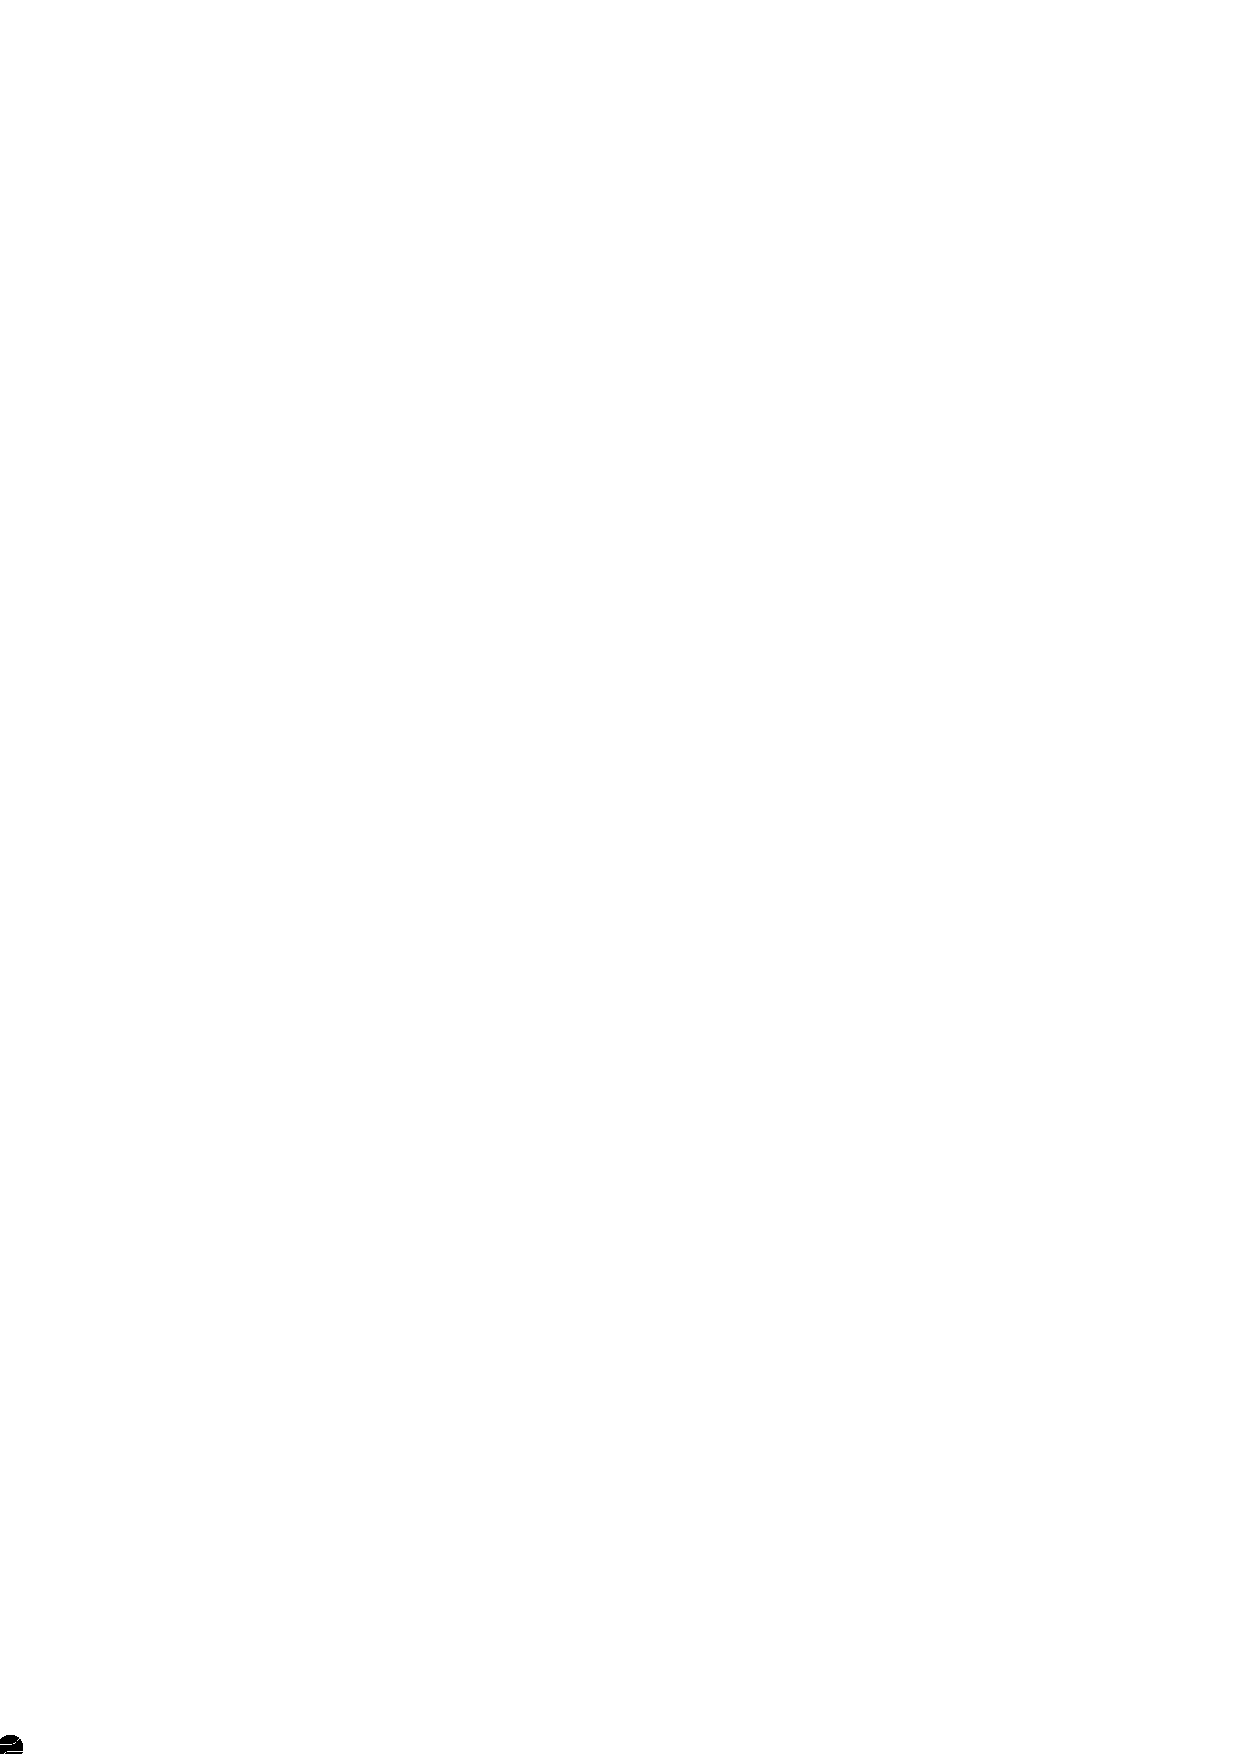
\includegraphics{ch0/FIG/smalletri.png} ETRI}
%\lfoot{무단복제금지 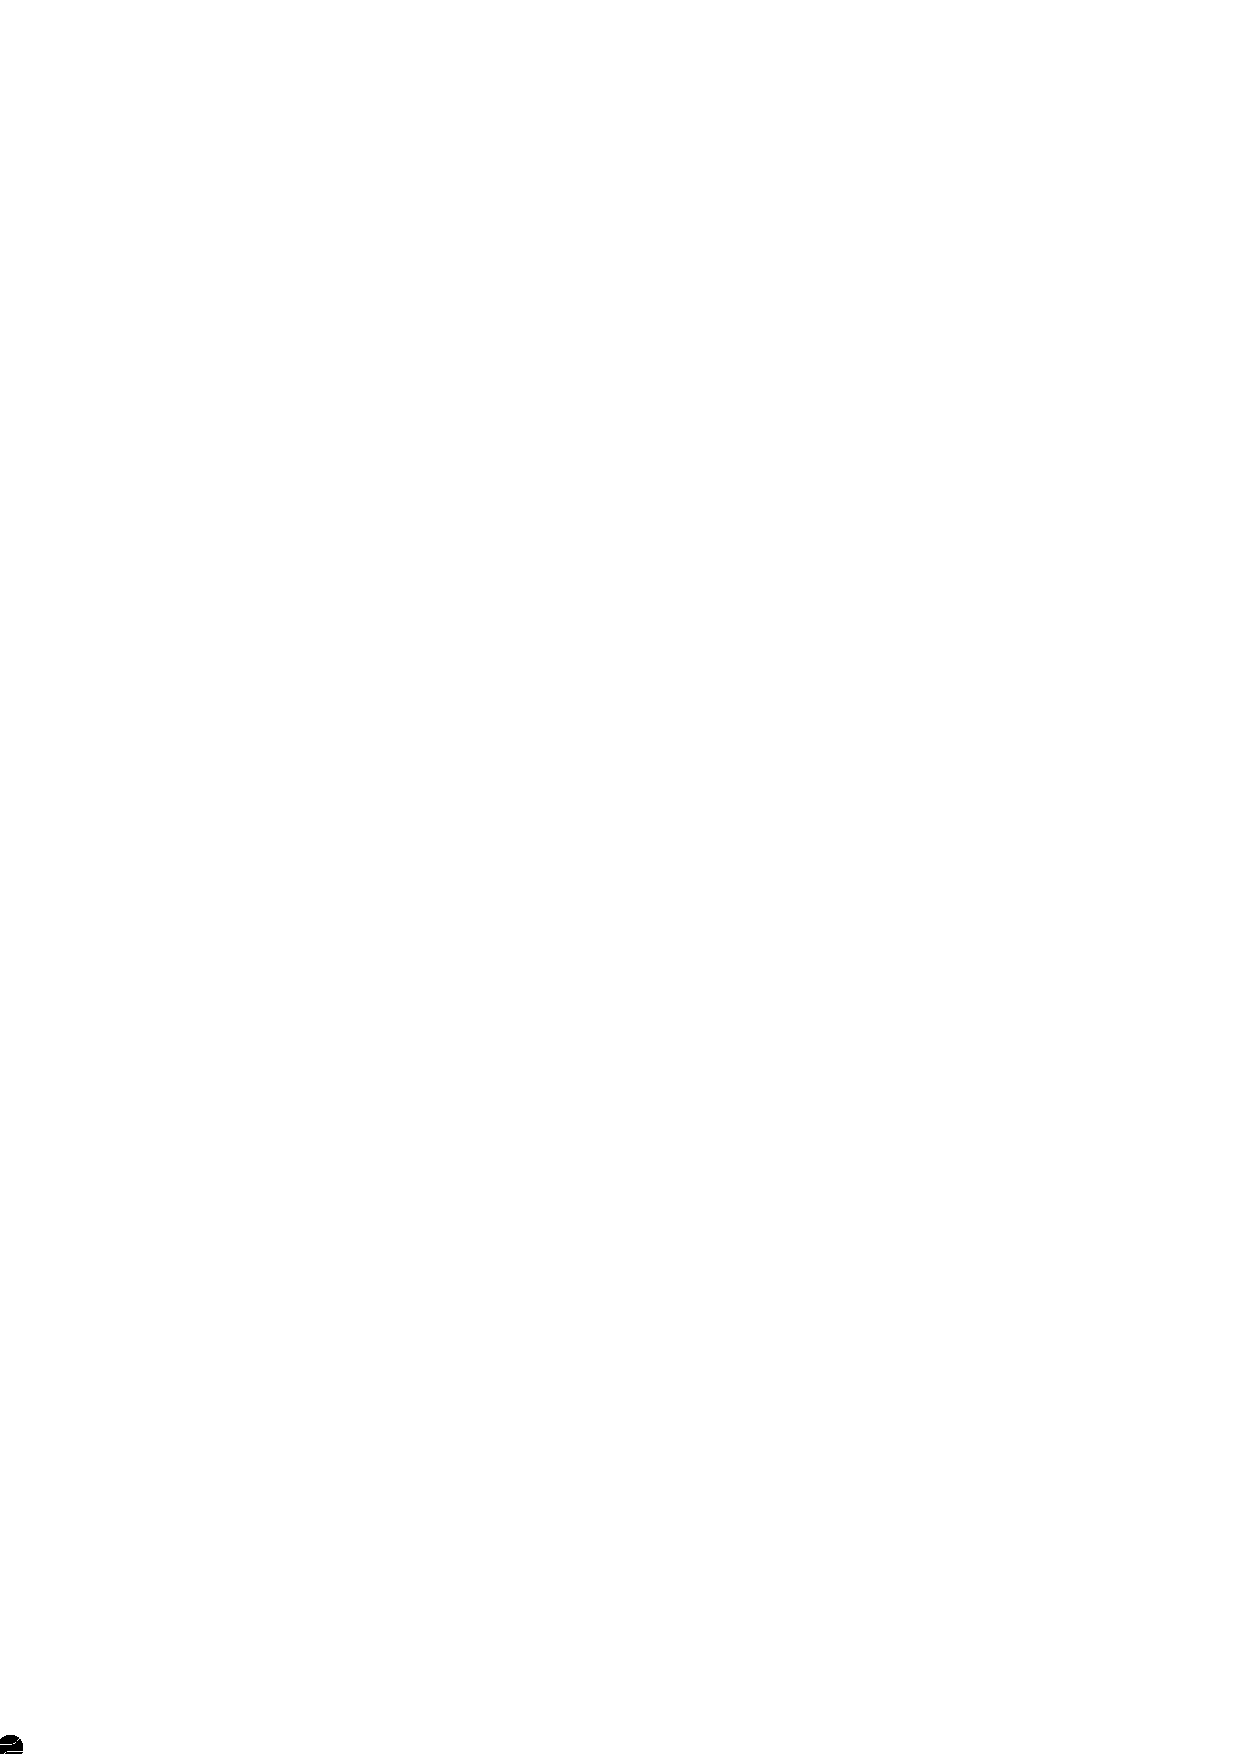
\includegraphics{ch0/FIG/smalletri.png} ETRI Proprietary}
%\lfoot{무단복제금지 ETRI Proprietary}
\cfoot{}
\rfoot{\thepage}
\setcounter{secnumdepth}{4}
\setcounter{tocdepth}{4}
\hypersetup{
    colorlinks=true, %set true if you want colored links
    linktoc=all,     %set to all if you want both sections and subsections linked
    linkcolor=blue,  %choose some color if you want links to stand out
}
%\hypersetup{linktocpage}
%
%\nofiles
%
\def\HB{HiPi+Bus}	% define system bus name
%%%
%%%%
%\draftcopySetGrey{0.8}
%\draftcopyName{Samsung Electronics}{50}
%\draftcopyName{LG Electronics Inc.}{50}
%\draftcopyName{School of Electrical Eng. / Korea University}{50}
%\draftcopyName{ETRI-CSTL}{50}
%\draftcopyName{UNIQUE / ETRI-CSTL}{50}
\SetWatermarkText{ETRI-CSTL}
\SetWatermarkScale{3}
%%%%
\begin{document}
%%%%%
\begin{titlepage}
\begin{center}{\LARGE\bf 시 스 템 버 스 블 록 설 계 서}\end{center}
\vspace{10mm}
\begin{center}{\Large\bf System Bus Block Specifications}\end{center}
\vspace{15mm}
\begin{center}{\Large\bf Ver.2.0}\end{center}
\vspace{15mm}
\begin{center}{\Large\bf 1994년 1월 20일}\end{center}
\vspace{15mm}
\begin{center}{\Large\bf 기 안 도}\end{center}
\vspace{15mm}
\begin{center}{\Large\bf 프 로 세 서 연 구 실}\end{center}
\begin{center}{\Large\bf 시 스 템 연 구 부}\end{center}
\begin{center}{\Large\bf 한 국 전 자 통 신 연 구 소}\end{center}
\begin{table}[b]
   \begin{center}
     \begin{tabular}{|l|} \hline
	\multicolumn{1}{|c|}{Copyright \copyright 1991$\bullet$1992$\bullet$1993$\bullet$1994 ETRI} \\
	이 보고서의 내용을 임의로 전재 또는 복사할 수 없으며, 이 보고서의 내용을 \\
	이용 또는 전재할 경우 반드시 한국전자통신연구소의 서면 허락을 먼저 취득 \\
	하여야 한다. \\ \hline
     \end{tabular}
   \end{center}
\end{table}
\thispagestyle{empty}
\end{titlepage}
%
%%%%%
\includepdf{td/td.pdf}
%%%%%
\clearpage
\pagenumbering{roman}
\tableofcontents
\addcontentsline{toc}{chapter}{목차}
\newpage
\listoffigures
\addcontentsline{toc}{chapter}{그림목차}
\newpage
\listoftables
\addcontentsline{toc}{chapter}{표목차}
%
\newpage
\chapter*{변경이력}
\addcontentsline{toc}{chapter}{변경이력}
%
\begin{enumerate}
  \item 1993년 2월 12일 : Ver.1.0 작성완료
  \item 1993년 2월 22일 : BLK103-21-1.0 문서등록
  \item 1993년 8월 16일 : Ver.1.1 작성완료
	\begin{itemize}
	  \item 오자교정
	  \item BCLK$<$9..0$>$*를 BCLK*로 변경
	  \item DI$<$7..0$>$*의 의미를 확장함 (표3.10 참고)
	  \item WRB 전송형태의 의미를 확장함 (제3.2.1장 Transfer Type 설명 참고)
	  \item 제7장 전기적 규격에 TTL 관련 규격을 추가함
	  \item 제8장 기계적 규격의 내용을 변경함
	  \item 부록을 추가함
	\end{itemize}
  \item 1993년 8월 23일 : BLK103-21-1.1 문서등록
  \item 1993년 12월 16일 : Ver.2.0 작성완료
	\begin{itemize}
	  \item 오자교정
	  \item 제3장 데이터전송버스의 내용중 BE$<$15..0$>$* 부분 변경
	  \item 제8장 기계적 규격의 내용중 백플레인 크기와 주보드 크기를 정정함
	\end{itemize}
\end{enumerate}
%%
\clearpage
\pagenumbering{arabic}
%%%%%
%%Title: HiPi+Bus V0.2 Chapter 1
%%Creator: Ando Ki
%%CreationDate: April 1992
%%FileName: ch1
%%RelatedFile: sec1 sec2
%%%%%
%
\chapter{HiPi+Bus}
%
%%%%%
%%Title: HiPi+Bus V0.2 Chapter 1 Section 1
%%Creator: Ando Ki
%%CreationDate: April 1992
%%FileName: sec1
%%RelatedFile: ch1
%%%%%
\section{서론}
\subsection{개발 목적 및 내용}
공유메모리를 사용하는 다중프로세서 구조를 갖는 시스템에서 프로세서와 메모리 사이의
정보 통로로 사용할 공유버스를 설계하는 것이 본 문서의 목적이다.
\HB\footnote{Highly Pipelined Plus Bus : \HB :
/hai-pai-pl\'{$\land$}s-b$\land$s/}는 시스템 버스이며,
이러한 시스템 버스를 설계하는 목표는 다음과 같다.
\begin{itemize}
  \item 공유메모리 다중프로세서 구조를 지원 \\
	공유메모리를 사용하는 다중프로세서 구조에서 프로세서와 메모리를 버스를
	이용하여 연결시킬때 시스템 버스는 데이터 전송 프로토콜, 전송속도,
	중재방법, 그리고 인터럽트 등 버스의 각 부분에서 다중프로세서를 지원하기
	위한 고려가 필요하다.
  \item 고성능 컴퓨터 지원 \\
	목표로하는 다중프로세서의 성능이 고성능이기 위해서는 시스템 버스도 이에
	어울리는 성능과 기능을 제공해야 하며 이를 위해 데이터 전송 능력,
	데이터 전송의 신뢰도, 시스템 구성 능력, 시스템 유지 보수를 위한 기능 등이
	고려되어야 한다.
\end{itemize}
\subsection{본 문서의 구성}
본 문서의 구성은 제 1 장에서 전체적인 구성과 설계 개념을 기술하고,
제 2 장에는 중재버스, 제 3 장에는 데이터 전송 버스, 제 4 장에는
인터럽트 버스, 제 5 장에는 유틸리티 버스, 제 6 장에는 시간 규격,
제 7 장에는 전기적 규격, 제 8 장에는 기계적 규격을 담고 있다.
\subsection{관련문서}
\begin{description}
  \item[(1)] 고속중형컴퓨터 (주전산기 III) 요구사항 정의서, SYS000-20-3.0,
	컴퓨터시스템연구실, 시스템공학연구부, 한국전자통신연구소, 1993.
  \item[(2)] 고속중형컴퓨터 (주전산기 III) 시스템 설계서, SYS000-21-3.0,
	컴퓨터시스템연구실, 시스템공학연구부, 한국전자통신연구소, 1993.
  \item[(3)] 고속중형컴퓨터 (주전산기 III) 하드웨어 서브시스템 설계서, SUS100-21-2.0,
	컴퓨터시스템연구실, 시스템공학연구부, 한국전자통신연구소, 1994.1.
\end{description}
\subsection{문서트리}
%
\begin{figure}[htb]
%\begin{center}
  \begin{picture}(400,170)(-200,-170)
	\thicklines
	\put(-50,-30){\framebox(100,20){요구사항 정의서}}
	\put(-50,-70){\framebox(100,20){시스템 설계서}}
	\put(-194,-110){\framebox(144,20){하드웨어 서브시스템 설계서}}
	\put(50,-110){\framebox(144,20){소프트웨어 서브시스템 설계서}}
	\put(-196,-171){\framebox(72,32){}} %외곽박스
	\put(-195,-170){\framebox(70,30){}}
		\put(-160,-153.5){\makebox(0,0)[b]{시스템버스}}
		\put(-160,-156.5){\makebox(0,0)[t]{블록설계서}}
	\put(-115,-170){\framebox(70,30){}}
		\put(-80,-153.5){\makebox(0,0)[b]{주처리장치}}
		\put(-80,-156.5){\makebox(0,0)[t]{블록설계서}}
	\put(-35,-170){\framebox(70,30){}}
		\put(0,-153.5){\makebox(0,0)[b]{주기억장치}}
		\put(0,-156.5){\makebox(0,0)[t]{블록설계서}}
	\put(45,-170){\framebox(70,30){}}
		\put(80,-153.5){\makebox(0,0)[b]{시스템제어기}}
		\put(80,-156.5){\makebox(0,0)[t]{블록설계서}}
	\put(125,-170){\framebox(70,30){}}
		\put(160,-153.5){\makebox(0,0)[b]{입출력처리기}}
		\put(160,-156.5){\makebox(0,0)[t]{블록설계서}}
	\put(0,-30){\line(0,-1){20}}
	\put(0,-70){\line(0,-1){10}}
	\put(-122,-80){\line(1,0){244}}
	  \put(-122,-80){\line(0,-1){10}}
	  \put(122,-80){\line(0,-1){10}}
	\put(-160,-125){\line(1,0){320}}
	  \put(-122,-110){\line(0,-1){15}}
	  \put(-160,-125){\line(0,-1){15}}
	  \put(-80,-125){\line(0,-1){15}}
	  \put(0,-125){\line(0,-1){15}}
	  \put(80,-125){\line(0,-1){15}}
	  \put(160,-125){\line(0,-1){15}}
  \end{picture}
%\end{center}
  \caption{문서트리}\label{figure:doc-tree}
\end{figure}
%

\subsection{참고자료}
\begin{description}
  \item[(1)] 컴퓨터구조연구실, {\em TICOM 시스템 버스 사용자 지침서 (TD88-6121-133.B)},
	시스템구조연구부, 한국전자통신연구소, 1990.11.
  \item[(2)] 컴퓨터구조연구실, {\em 시스템 버스 표준 인터페이스 설계서 Ver.2.0 (TM93-CA-017.B)},
	시스템구조연구부, 한국전자통신연구소, 1993.7.
  \item[(3)] 컴퓨터구조연구실, {\em TTL 회로 설계의 고려사항 (TM92-CA-039)},
	시스템구조연구부, 한국전자통신연구소, 1992.6.26.
  \item[(4)] 컴퓨터구조연구실, {\em HiPi+Bus의 임계시간 (TM92-CA-053)},
	시스템구조연구부, 한국전자통신연구소, 1992.11.16.
  \item[(5)] 컴퓨터구조연구실, {\em BTL 기초조사 (TM93-CA-001.B)},
	시스템구조연구부, 한국전자통신연구소, 1993.2.
  \item[(6)] IEEE, {\em IEEE Standard Test Access Port
	and Boundary-Scan Architecture}, IEEE std.1149.1, 1990.
  \item[(7)] IEEE, {\em IEEE Standard for Electrical Characteristics of
	Backplane Transceiver Logic (BTL) Interface Circuits},
	IEEE std.1194.1, 1991.
  \item[(8)] 컴퓨터구조연구실, {\em Semaphore Cache {\it (Draft)\/}},
	시스템구조연구부, 한국전자통신연구소, 1993.
  \item[(9)] 컴퓨터구조연구실, {\em 인터럽트 관련 모듈 설계서 {\it (Draft)\/}},
	시스템구조연구부, 한국전자통신연구소, 1993.
  \item[(10)] 컴퓨터구조연구실, {\em 고속중형컴퓨터 클럭 서브 시스템 (TM93-CA-020)},
	시스템구조연구부, 한국전자통신연구소, 1993.4.
\end{description}
%
%%%%%

\newpage
%%%%%
%%Title: HiPi+Bus V0.2 Chapter 1 Section 2
%%Creator: Ando Ki
%%CreationDate: April 1992
%%FileName: sec2
%%RelatedFile: ch1
%%%%%
\section{블록 설계 개념}
\subsection{다중 프로세서를 지원하기 위한 고려사항}
\begin{itemize}
	\item Pended Protocols \\
		Pended 프로토콜은 하나의 데이터 전송을
		요청 단계(request phase)와 응답 단계(respond phase)로
		나눔으로써 메모리 접근 시간이 버스의 전송 속도(bus bandwidth)에
		영향을 주지 않도록 하는 방법이다. 
		메모리를 접근하는 동안 하나의 프로세서가 계속해서 버스를 점유하는
		것이 아니므로, 
		다수의 데이터 전송 요청이 동시에 발생할 수 있는 
		다중 프로세서 환경에서는 이 프로토콜이 절대적으로 유리하다.
	\item Synchronous - 16.5 MHz \\
		Pended 프로토콜은 데이터 전송을 요청과 응답의 두 단계로
		나누어 pipeline시킨 것이다.
		따라서 이와 같은 프로토콜을 구현하기에는 비동기형 제어 방식보다는 
		동기형 제어방식이 유리하다.
		동기형 제어 방식은 비동기형에 방식에 비해 기술의 발전에 따른 
		탄력적 성능 향상을 얻기 어렵지만, 신뢰도가 높고
		현재의 기술로 비동기형보다 나은 성능을 발휘할 수 있도록
		구현할 수 있다는 장점을 가지고 있다.
		클럭 주기는 단위 버스 동작이 수행되는 시간을 말하는
		것으로 60.6 {\it n\/}sec이다.
	\item Fairness arbitration \\
		다중 프로세서 시스템의 가장 큰 장점 중의 하나는 여러개의
		프로세서가 일을 분담하여 수행함으로써 얻어지는 
		빠른 응답이라 할 수 있다. 이와 같은 장점을 충분히 발휘하도록
		하기 위해서는 모든 프로세서가 동등한 자격을 갖고
		매 순간마다 일의 균형있는 분배 (dynamic load balancing)가
		이루어져야 한다.
		균형 분배는 운영 체제에서 많은 책임을 갖고 있지만,
		우선 하드웨어 수준에서의 동등한 자원 공유가 보장되어야 가능하다.
		버스는 가장 핵심이 되는 자원이므로 버스 사용의 공정한 중재가
		균형 분배의 시발점이라 할 수 있다.
		\HB에는 모든 버스 모듈이 공정하게
		버스를 사용할 수 있도록 중재 규칙을 정의하였다.
	\item Cache Coherency Protocols \\
		버스를 사용하는 모든 다중 프로세서 시스템의 가장 큰 문제는
		버스의 포화에 의한 시스템 성능 저하이다.
		버스가 포화되면 프로세서 수가 증가하여도 시스템의 성능은
		향상되지 않고 오히려 감소되기 때문이다.
		이와 같은 문제를 해결하기 위한 방법으로 공유 메모리를 사용하는
		다중 프로세서 시스템에서는 각 프로세서가 캐쉬를 갖게
		하여 캐쉬에 원하는 데이터가 존재하지 않을 경우에 한해서
		버스를 사용하게 함으로써 버스의 포화를 방지한다.
		그러나 프로세서마다 독립적으로 캐쉬를 사용하게 되면 
		캐쉬상에 존재하는 데이타가 메모리나 다른 캐쉬의 데이타와
		일관성이 깨어지는 문제(multi-cache consistency problem)가
		발생할 수 있으므로 이 문제를 해결하여야 한다.
		\HB에서는 write-back
		캐쉬의 동일성 유지 프로토콜을 지원한다.
	\item Interlock Protocols \\
		다중처리에서 필수적인 동기화를 지원하기 위한 잠금 프로토콜을 지원한다.
	\item Interrupt Broadcast and Arbitration \\
		공유 메모리를 사용하는 다중 처리 시스템 환경에 있어서의
		모든 프로세서들은 동등한 자격을 갖고 
		동작한다. 따라서 인터럽트의 요구와 처리에 있어서 단일
		프로세서 시스템과는 다른 기능들이 필요하게 된다.
		즉, 여러 프로세서가 모두 인터럽트를 처리할 수 있기 때문에
		여러 프로세서로 인터럽트를 보내는 방법(broadcast)과
		실질적으로 인터럽트를 처리할 프로세서를 선정하는
		기능(arbitration)이 필요하다.
		\HB는 이와 같은 인터럽트의 기능들을 제공하고 있으며,
		인터럽트를 모든 프로세서들 사이의
		비동기적인 통신 수단으로 이용할 수 있도록 일반화시켰다.
\end{itemize}
\subsection{고성능 버스를 위한 고려사항}
\begin{itemize}
	\item Bus bandwidth - 264 Mbytes/sec \\
		\HB는 264 Mbytes/sec의 지속적인 전송 용량(sustained
		bus bandwidth)을 갖는다.
	\item 128 bit data + 32 bit address, NonMultiplexed \\
		\HB는 128 비트의 데이터 전송을 위한 신호와
		32 비트 어드레스 전송을 위한 신호를 
		별도로 갖고 있다. 따라서 어드레스 전송을 위해 데이터의 전송선을
		사용하지 않기 때문에
		매 버스 클럭 주기(60.6 {\it n\/}sec)마다 128 비트의 데이터가
		전송될 수 있어서 264 Mbytes/sec의 
		데이터 전송 속도를 얻을 수 있다.
		32 비트의 어드레스 전송선을 갖기 때문에
		최대 4 Gbytes의 연속적인 어드레스 영역을 지원한다.
	\item Block Transfer \\
		캐쉬 라인 크기와 같은 크기인 64바이트 전송을 지원한다.
	\item All bytes are parity protected \\
		시스템의 신뢰도 향상을 위하여 버스에서는 모든 신호에
		에러 방어를 위한 신호를 추가한다.
		에러 방어의 대상은 순간적인 에러(transient or soft error)이며
		재시도(retry)에 의해 처리한다.
		고장으로 인한 계속적인 에러에 대해서는 처리 방법을 버스 규격에서
		별도로 정의하지 않는다.
		기본적으로 버스의 모든 신호는 바이트 단위의 패리티 비트를 갖는다.
		단, 신호의 특성상 바이트 단위로 동시에 구동되지 않는
		신호의 경우는 예외로 한다.
	\item 21 slots \\
		하나의 보드는 하나의 슬롯을 이용하여 버스상에 장착된다.
		따라서 슬롯의 수는 버스에 장착될 수 있는 최대 보드의 수를 말하고
		이것은 시스템의 구성을 제한한다.
		21 개의 슬롯은 13 개의 프로세서 보드 (데이터 처리 프로세서와 입출력 프로세서)와
		8 개의 메모리 보드가 장착되도록 한다.
	\item No mechanical switch and jumper \\
		이전에는 버스나 버스 모듈에
		다소의 유연성을 제공하기 위하여 기계적인 스윗치나 점퍼를 많이 사용되었다. 
		그러나 기계적 부품은 다른 부품에 비하여 신뢰도가 많이 떨어지기
		때문에 많은 시스템 고장의 원인이 되어왔다.
		이와 같은 이유로 \HB에서는 기계적인 부품을 없애고
		소프트웨어 제어가 가능한 레지스터를 사용하여 스윗치를 대신한다.
	\item BTL (Backplane Transceiver Logic) \\
		백플레인 구동에는 BTL 기술을 사용한다.
	\item I/O connector \\
		백플레인에 입출력 버스와의 연결을 용이하게 하기 위한 콘넥터를 둔다.
\end{itemize}
%%%%%

\newpage
%%%%%
%%Title: HiPi+Bus V0.2 Chapter 1 Section 4
%%Creator: Ando Ki
%%CreationDate: April 1992
%%FileName: sec3
%%RelatedFile: ch1
%%%%%
\section{블록 구조}

\subsection{관련 블록 간 구조}
시스템 버스 블록(BUS block)은 {\tt <}그림~\ref{figure:block-relation}{\tt >}에서
굵은 선으로 표시된 부분에 해당한다.
%
%
%\documentstyle[11pt,doublespace,a4wide,psfig]{harticle}
%\setstretch{1.2}
%\pagestyle{headings}
%\begin{document}
%
%
\begin{figure}[htb]
%\begin{center}
  \begin{picture}(370,140)(0,-70)
	\thicklines
	\put(40,0){\oval(82,22)} %외곽박스
	\put(40,0){\oval(80,20)\makebox(0,0){시스템버스블록}}
	\put(145,60){\oval(90,20)\makebox(0,0){주처리장치블록}}
	\put(145,30){\oval(90,20)\makebox(0,0){주기억장치블록}}
	\put(145,0){\oval(90,20)\makebox(0,0){입출력처리기블록}}
	\put(145,-30){\oval(90,20)\makebox(0,0){시스템제어기블록}}
	\put(145,-60){\oval(90,20)\makebox(0,0){패키징블록}}
	\put(260,15){\oval(80,20)\makebox(0,0){고장진단블록}}
	\put(260,-15){\oval(80,20)\makebox(0,0){펨웨어블록}}
	\put(360,0){\oval(80,40)}
		\put(360,8){\makebox(0,0){입출력제어기/}}
		\put(360,-9){\makebox(0,0){디바이스블록}}
	\put(80,0){\line(1,3){20}}
	\put(80,0){\line(2,3){20}}
	\put(80,0){\line(1,0){20}}
	\put(80,0){\line(2,-3){20}}
	\put(80,0){\line(1,-3){20}}
	\put(190,60){\line(2,-3){30}}
	\put(190,30){\line(2,-1){30}}
	\put(190,0){\line(2,1){30}}
	\put(190,-30){\line(2,3){30}}
	\put(190,0){\line(2,-1){30}}
	\put(190,-30){\line(2,1){30}}
	\put(250,5){\line(0,-1){10}}
	\put(300,15){\line(2,-1){20}}
	\put(300,-15){\line(2,1){20}}
  \end{picture}
%\end{center}
  \caption{하드웨어 서브시스템의 블록 간 상호관계}\label{figure:block-relation}
\end{figure}
%
%\end{document}
%%%%%

%
즉 하드웨어 서브시스템에서 주 처리 장치 블록(MPU block),
주 기억 장치 블록(MEM block), 입출력 처리기 블록(IOP block), 시스템
제어기 블록(SCM block), 그리고 패키징 블록(PAC block)이 전기적, 기계적, 기능적으로
백플레인에 의해 연결될 때 이 백플레인을
포함한 전기적, 기계적, 기능적 집합체를 시스템 버스 블록이라 한다.

\subsection{시스템의 구성}
공유메모리를 갖는 다중 프로세서 시스템의 시스템 버스인 
\HB는
프로세스, 메모리, 기타 버스 상에 장착되는 보드들 사이의 정보 교환 통로로써 이용된다.
%
\begin{figure}[htb]
    \centerline{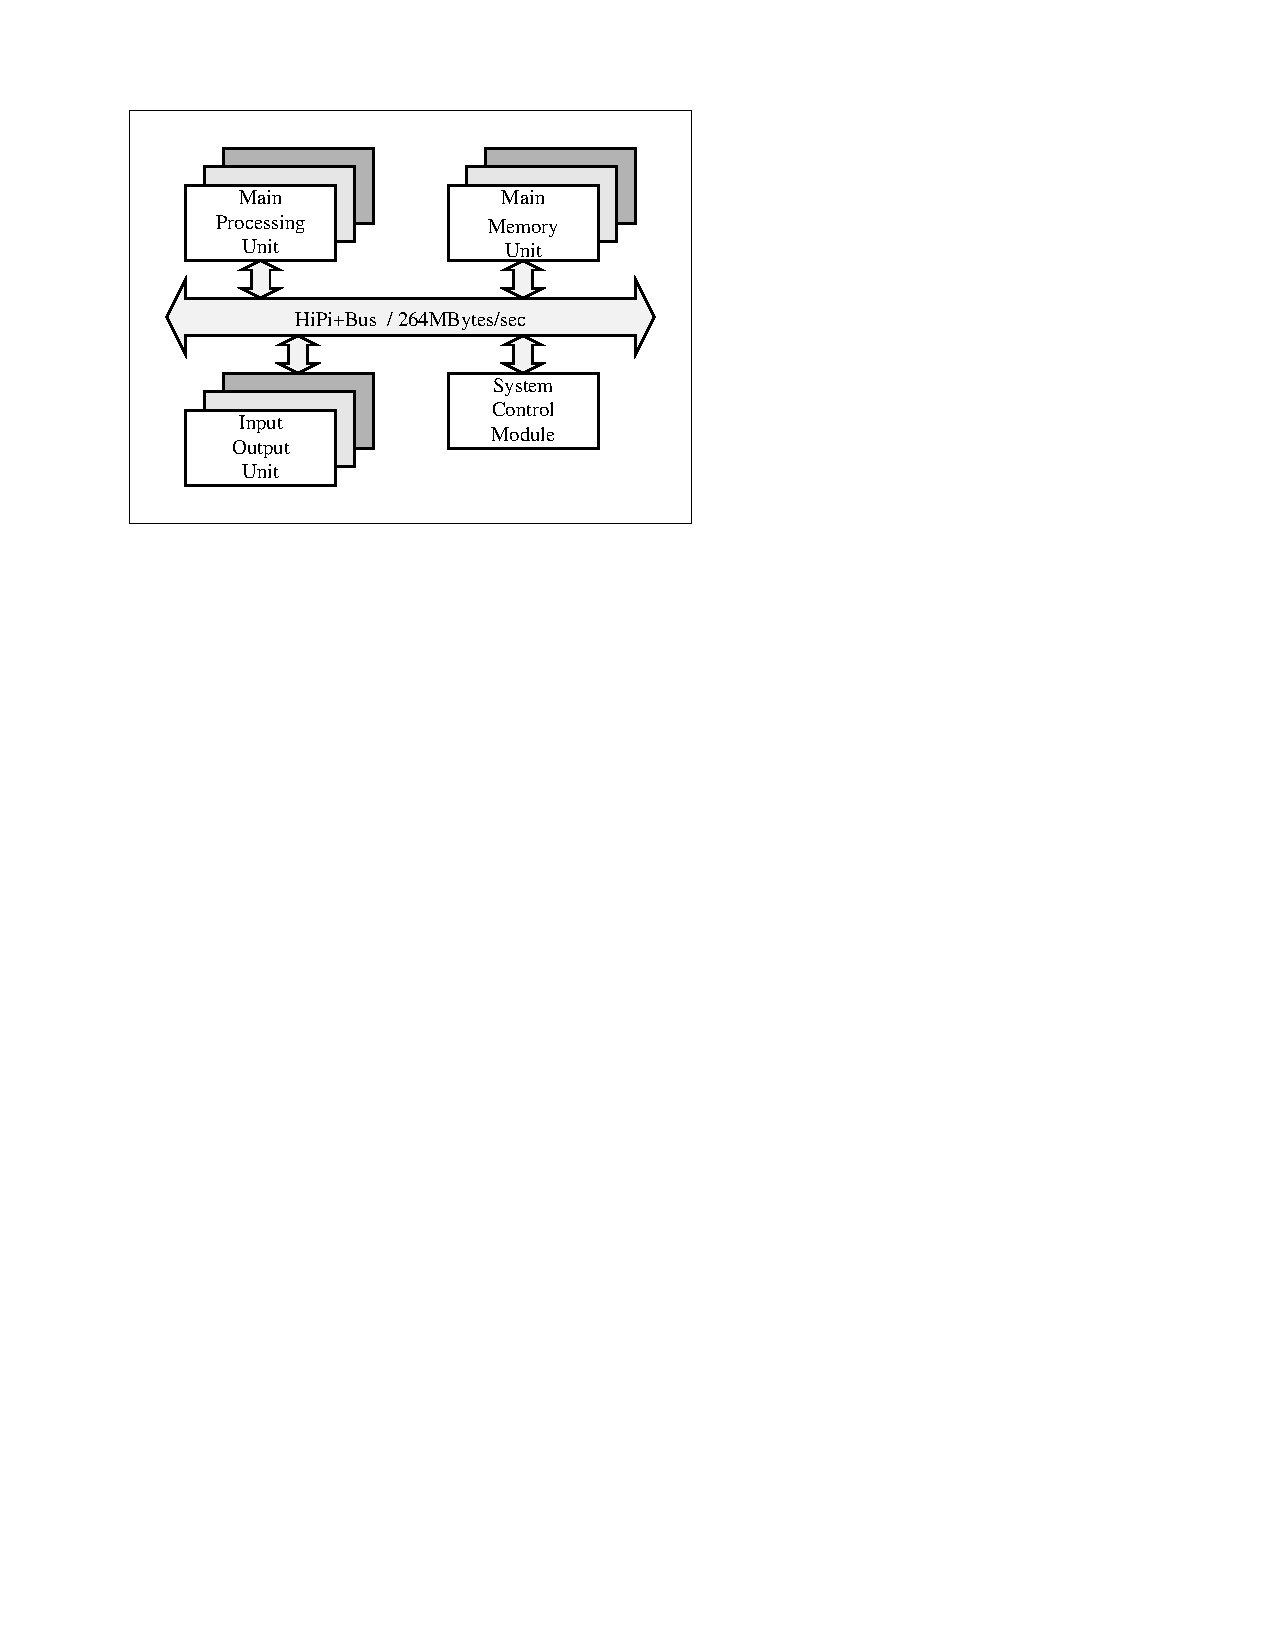
\includegraphics[height=3.5in]{ch1/FIG/system.jpg}} %\centerline{\psfig{figure=ch1/FIG/system.ps,height=3.5in}}
   \caption{시스템 구성}\label{figure:system-config}
\end{figure}
%

\subsection{주요규격}
시스템 버스 블록(BUS block)의 주요규격은 {\tt <}표~\ref{table:bus-spec}{\tt >}와
같다.
%
\begin{table}[htbp]
\caption{\HB의 규격}\label{table:bus-spec}
  \begin{center}
\begingroup
\setlength{\tabcolsep}{6pt} % Default value: 6pt
\renewcommand{\arraystretch}{0.9} % Default value: 1
  \begin{tabular}{|l l|} \hline
   \multicolumn{2}{|c|}{중재 특성 (Characteristics of Arbitration)} \\ \hline
      중재 규칙 & 우선순위와 공정성 (Priority and Fairness) \\
      중재 수행 시간 & 1 Bus Clock (60.6 {\it n\/}sec) \\
      중재 기법 & 선형자가중재 (Linear Self Arbitration) \\
      중재기의 특성 & 분산형 중재기 (Distributed Arbiter) \\
      기타 & Request Inhibition, Request Timeout 구현 \\ \hline
   \multicolumn{2}{|c|}{데이터 전송 특성 (Characteristics of Data Transfer)} \\ \hline
      프로토콜 & 펜디드 (Pended) \\
      제어 방식 & 동기형 (Synchronous) \\
      클럭 속도 & 16.5 MHz (60.6 {\it n\/}sec) \\
      어드레스/데이터 & non-multiplexed \\
      최대 어드레스 영역의 크기 & 4 Gbytes (32 bits wide) \\
      어드레스 영역의 갯수 & 8 (3개 정의) \\
      최대 사용 가능한 전송 형태 & 32 (13개 정의) \\
      버스의 폭 (Bus Width) & 128 bits (16 bytes) \\
      데이터의 단위 (Data Unit) & 8 bits (1 byte) \\
      전송 가능한 데이터의 크기 & 16-바이트 이내의 연속된 바이트; 64-바이트 \\
      정렬의 제약 (Alignment Restriction) & 16 byte boundary; 64 byte boundary \\
      Justification & Straight (Nonjustified) \\
      데이터 전송 속도(Data Transfer Rate) & 264 Mbytes/sec ($16Bytes \times 16.5M\!H\!z$)\\ \hline
   \multicolumn{2}{|c|}{인터럽트 전송 특성 (Characteristics for Interrupt Transfer)} \\ \hline
      전송 프로토콜 & Message passing protocols \\
      제어 방식 & 동기형 (Synchronous) \\
      클럭 속도 & 16.5 MHz (60.6 {\it n\/}sec) \\
      전송 속도 & 최대 약 1.6 MI/sec (Mega Interrupts per second) \\
      중재 기법 & 부호화된 자가중재 (Coded Self Arbitration) \\
      중재기 특성 & 분산형 중재기 (Distributed Arbiter) \\
      에러 방어 & Parity Detection \\
      기타 & Broadcast and Arbitration \\ \hline
    \multicolumn{2}{|c|}{기 타 (Etc.)} \\ \hline
      캐쉬 지원 & Write Back Cache Coherency Protocol \\
      동기화 지원 (Synchronization) & Semaphore Cache Protocol \\
      에러 검출 (Error Detection) & 바이트 단위의 홀수 패리티(odd parity) \\
      에러 처리 (Error Handling) & 재시도 (Retry) \\
      경계주사 (Boundary Scan) & IEEE std.1149.1 \\
      구현 기술 (Technology) & BTL (IEEE std.1194.1) \\
      슬롯 수 & 21 slots/backplane \\
      콘넥터 규격 & 85$\times$4rows (340pins, 전원제외)\\
                  & 40$\times$4rows (160pins, 전원포함)\\
      공급 전원 & +5V, +5V Standby \\
      총 신호수 & 293 (전원제외, 입출력용 제외) \\ \hline
  \end{tabular}
\endgroup
  \end{center}
\end{table}
%


\subsection{블록의 구조}
시스템 버스 블록(BUS block)은 {\tt <}그림~\ref{figure:block}{\tt >}와
같이 크게 중재버스(arbitration bus), 데이터 전송버스(dtat transfer bus),
인터럽트 전송버스(interrupt transfer bus), 그리고 유틸리티 버스(utility bus)로
구분된다.
%
\begin{figure}[htb]
    \centerline{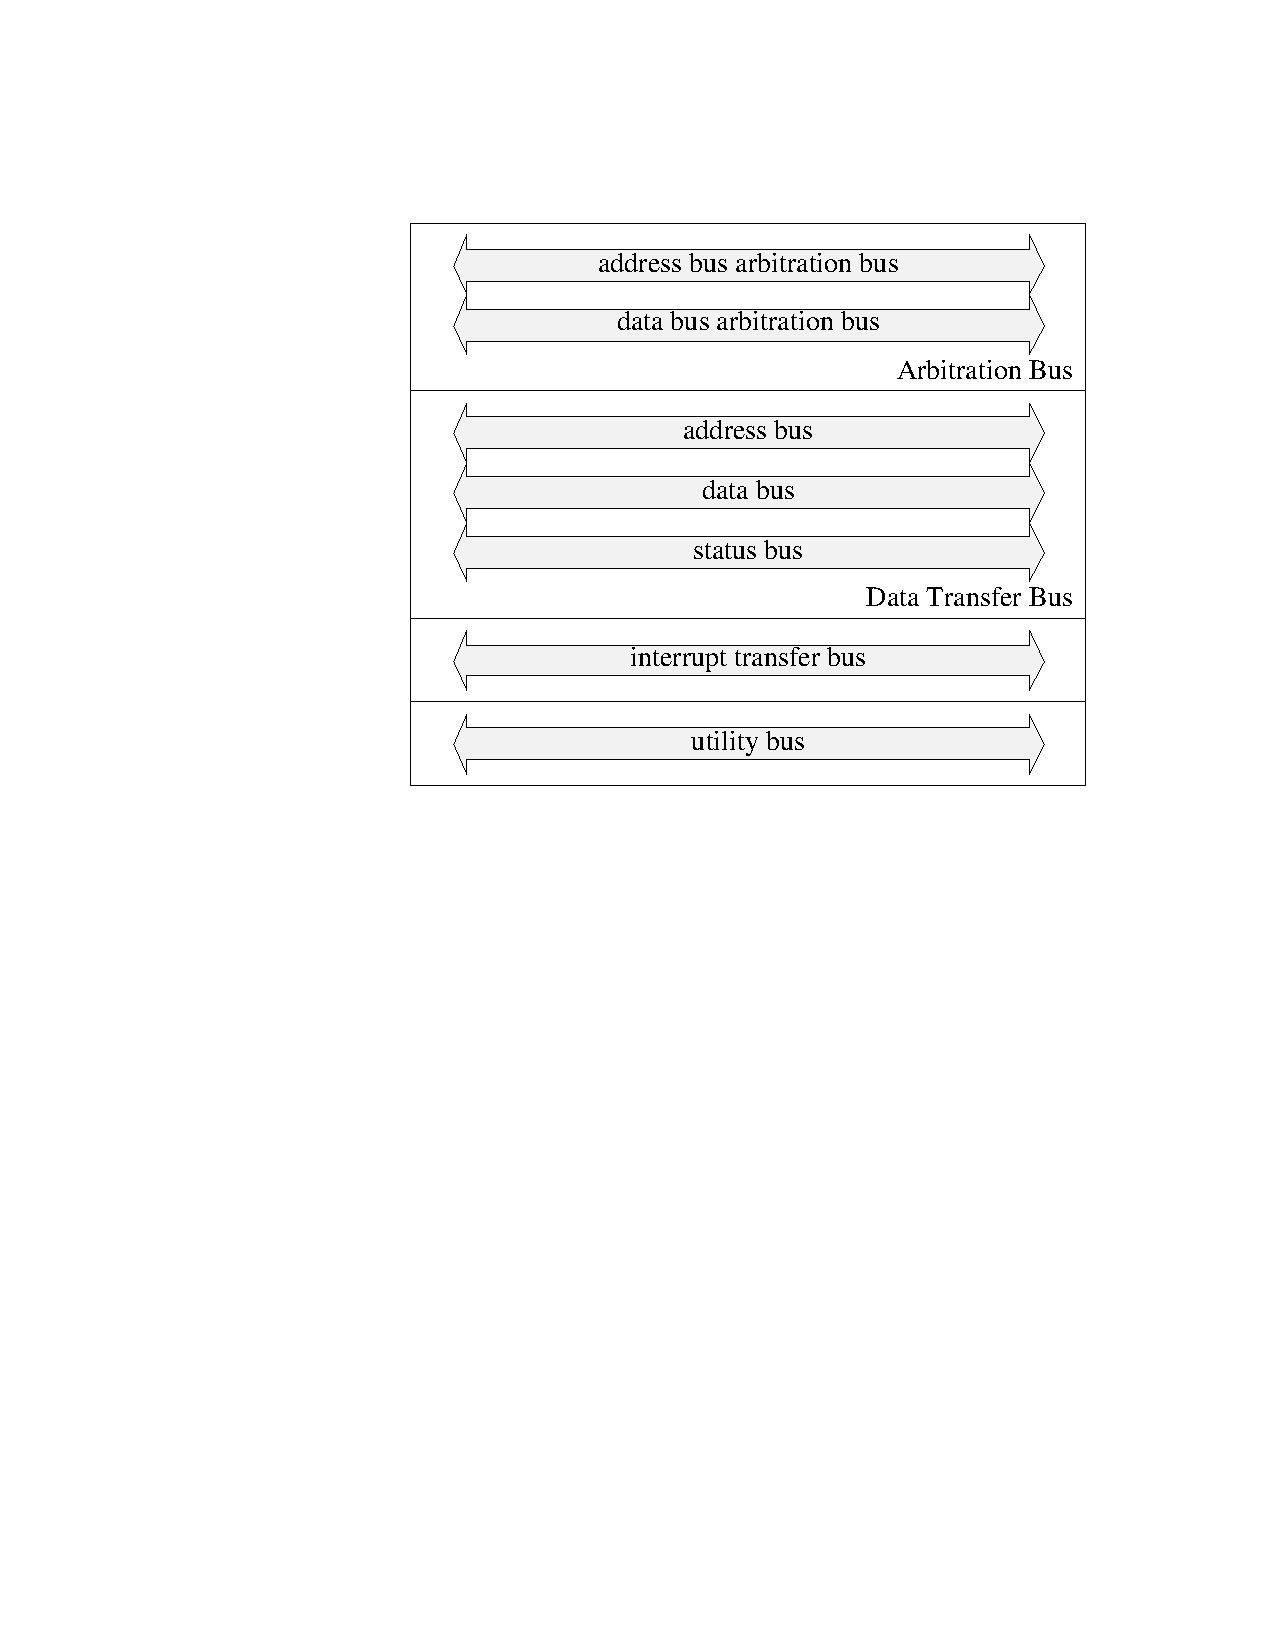
\includegraphics{ch1/FIG/block.jpg}} %\centerline{\psfig{figure=ch1/FIG/block.ps}}
   \caption{버스 블록의 구조}\label{figure:block}
\end{figure}
%
그리고 중재버스는 어드레스 버스 중재버스(address bus arbitration bus)와
데이터 버스 중재버스(data bus arbitration bus)로 구성되고,
데이터 전송버스는 어드레스 버스(address bus), 데이터 버스(data bus),
그리고 상태 버스(status bus)로 구성된다.

\subsection{버스신호들}
시스템 버스에서 정의하여 사용하는 버스 신호들은 {\tt <}표~\ref{table:signals}{\tt >}와
같다.
%\documentstyle[11pt,a4]{hbook}
%\begin{document}
%
\begin{table}[htbp]
\caption{신호선들}\label{table:signals}
   \begin{center}
\begingroup
\setlength{\tabcolsep}{6pt} % Default value: 6pt
\renewcommand{\arraystretch}{0.9} % Default value: 1
   \begin{tabular}{|l|l|r|l|} \hline
Bus&Mnemonic & Size & Name \\ \hline \hline
     & {\bf ABRQ$<$12..0$>$*} & 13 & Address Bus Request \\
     & {\bf ABINH*}                    & 1 & Address Bus Arbitration Inhibition \\
중재버스 & {\bf WRINH*}                    & 1 & Write Cycle Inhibition \\
     & {\bf DBRQ$<$8..0$>$*}  & 9 & Data Bus Request \\
     & {\bf DBINH*}                    & 1 & Data Bus Arbitration Inhibition \\
     & {\bf PCW*}                      & 1 & Priority Change Window \\ \hline
         & {\bf A$<$31..4$>$*}     & 28 & Address \\
         & {\bf AP$<$3..0$>$*}     & 4 & Address Parity \\
         & {\bf SI$<$7..0$>$*}     & 8 & Source Identification \\
         & {\bf SIP*}                      & 1 & Source Identification Parity \\
데이터전송버스  & {\bf AS$<$2..0$>$*}     & 3 & Address Space \\
(어드레스버스) & {\bf TT$<$4..0$>$*}     & 5 & Transfer Types \\
         & {\bf STP*}                      & 1 & Space + Types Parity \\
         & {\bf BE$<$15..0$>$*}    & 16 & Byte Enable \\
         & {\bf BEP$<$1..0$>$*}    & 2 & Byte Enable Parity \\
         & {\bf AE*}                       & 1 & Address Cycle Enable \\ \hline
         & {\bf D$<$127..0$>$*}    & 128 & Data \\
데이터전송버스  & {\bf DP$<$15..0$>$*}    & 16 & Data Parity \\
(데이터버스)  & {\bf DI$<$7..0$>$*}     & 8 & Destination Identification \\
         & {\bf DIP*}                      & 1 & Destination Identification Parity \\
         & {\bf DE*}                       & 1 & Data Cycle Enable \\ \hline
        & {\bf AACK$<$1..0$>$*}   & 2 & Address Acknowledge \\
        & {\bf SHD*}                      & 1 & Hit on Shared Line \\
        & {\bf DTY*}                      & 1 & Hit on Dirty Line \\
데이터전송버스 & {\bf SNK*}                      & 1 & Snoop No Acknowledge \\
(상태버스)  & {\bf ITV*}                      & 1 & Intervention \\
        & {\bf LCR*}                      & 1 & Hit on Interlocked Region \\
        & {\bf DACK*}                     & 1 & Data Acknowledge \\
        & {\bf CDK*}                      & 1 & Cache Data Acknowledge \\
        & {\bf SPIN$<$3..0$>$*}   & 4 & Spin Queue Order \\
        & {\bf BSY$<$7..0$>$*}    & 8 & Busy Status Line \\ \hline    
인터럽트 & {\bf IBSYNC*}                   & 1 & Interrupt Bus Sync. \\
전송버스 & {\bf IBD$<$7..0$>$*}    & 8 & Interrupt Bus Data \\
     & {\bf IBDP*}                     & 1 & Interrupt Bus Data Parity \\ \hline
       & {\bf BCLK*}                   & 1 & Bus Clock \\
유틸리티버스 & {\bf RST*}                      & 1 & System Reset \\
       & {\bf SFAIL*}                    & 1 & System Fail \\
       & {\bf GA$<$4..0$>$*}     & 5 & Geographical Slot Address \\
       & {\bf Tx$<$4..0$>$}     & 5 & JTAG Boundary Scan Option \\ \hline
       & {\it total\/} & 293 & \\
\hline
   \end{tabular}
\endgroup
   \end{center}
\end{table}
%
%\end{document}
%%%%


\subsection{문서 작성의 규칙}

\subsubsection{신호 이름에 대한 규칙}
\begin{itemize}
  \item 버스 신호의 Mnemonics은 모두 대문자를 사용한다. \\
	예: AE*, DE*, A{\tt <}31..4{\tt >}*
  \item 버스 신호의 Mnemonics은 신호 이름 중에서 신호 이름을 대표할 수 있는 앞뒤 몇 문자를 사용한다. \\
	예: Bus Clock : BCLK*; Shared Line : SHD*
  \item 버스 상의 모든 신호의 끝에는 모두 *를 붙힌다. 이는 버스 신호의 전압이 낮은 상태일 때 
	``참 (true)''이 됨을 의미한다. \\
	예: A{\tt <}0{\tt >}*, DTY*
  \item 동일한 이름을 갖는 여러 비트의 신호는 {\tt <}{\tt >}을 사용하여 번호와 크기를 나타낸다. \\
	예: A{\tt <}31..4{\tt >}*,
	A{\tt <}4{\tt >}*, D{\tt <}127..0{\tt >}*, TT{\tt <}3{\tt >}*
  \item 번호는 큰 쪽을 먼저 쓰는 것을 기본(default)으로 한다. \\
	예: A{\tt <}31..4{\tt >}*, D{\tt <}127..0{\tt >}*,
	TT{\tt <}3..0{\tt >}*
  \item 동일 이름을 갖는 여러 비트의 신호중 임의의 한 신호 또는 한 비트를 지칭할 때는 {\tt <}n{\tt >}을 사용한다. \\
	예: A{\tt <}n{\tt >}*, D{\tt <}n{\tt >}*,TT{\tt <}n{\tt >}*
  \item 동일 이름을 갖는 여러 비트의 신호를 총칭할 때는 비트 폭을 모두 표시하거나 또는 비트 폭 표시가 없는
	Mnemonics만으로 표시한다. \\
	예: A{\tt <}31..4{\tt >}* 또는 A*; D{\tt <}127..0{\tt >}* 또는 D*
\end{itemize}
%

\subsubsection{신호의 상태에 대한 규칙}
\begin{itemize}
  \item 신호의 상태는 신호의 논리적인 값(``참''/``거짓'')을 표현하는 방법을 주로 사용하고,
	경우에 따라 버스상에 전압의 높낮음(``high''/``low'')으로 표현하는 방법을 사용한다.
  \item 신호의 논리적인 값을 표현하기 위하여 ``참'', ``거짓'', ``true'', ``false'', 
	T (True의 약자), F (False의 약자), 1, 0을 사용한다.
	``참'', ``true'', T, 1이 같은 값이고, ``거짓'', ``false'', F, 0이 같은 값이다.
	신호의 논리적인 값을 나타낼 때 신호 뒤에 붙는 *는 논리적인 값에 의미를 갖지 않는다. \\
	예: AE* = T, AE = 1, AE* = ``true'', AE* = ``low'', AE* = L : same state \\
	예: DE* = F, DE = 0, DE* = ``false'', DE* = ``high'', DE* = H : same state
  \item 신호의 상태 중 버스 상의 전압 레벨로 표현하기 위하여 ``high'', ``low'', H, L를 사용한다.
	이때 신호의 뒤에 붙는 *는 전압의 레벨를 반대로 하는 역할을 한다. \\
	예: AE* = ``high'', AE* = H, AE = L : same state \\
	예: DE* = ``low'', DE* = L, DE = H : same state
  \item 여러개의 신호가 모여서 의미를 갖는 상태를 나타낼 경우 그 신호의 논리적인
	값은 숫자로 표현할 수 있다. 이때 값의 표현 방법은 
	16진수(Hexadecimal)를 기본(default)으로 한다. \\
	16진수(Hexadecimal)를 나타내는 prefix로 `0x'를 사용한다. \\
	예: A{\tt <}31..4{\tt >}* = 12345,
	TT{\tt <}3..0{\tt >}* = 4, AS{\tt <}3..0{\tt >}* = 0x5
  \item 신호의 상태를 나타낼때 논리적인 값을 사용하는 것을 기본(default)으로 한다. 
	단, 신호의 시간적인 규격을 기술할 때는 전압 레벨을 사용한다(신호의 이름에 
	*의 유무 확인요).
\end{itemize}
%

\subsubsection{시간 규격 표시에 대한 규칙}
\begin{itemize}
  \item 시간 규격은 {\it n\/}sec ($10^{-9}$ 초)를 기본 단위로 한다.
	단, 예외의 경우는 별도로 시간 단위를 표시한다.
  \item 시간 규격에서 사용하는 신호의 타이밍도는 실제 버스에 나타나는 신호를 기준으로 
	설명함을 원칙으로 하고,
	다만 설명의 편의를 위해 구동소자에 관련된 동작을 부가적으로 표시한다.
\end{itemize}
%

\subsubsection{신호의 값을 지정하는 일반적인 규칙}
\begin{itemize}
  \item 신호의 값은 쉽게 구별되도록 지정한다. \\
	예 : TT{\tt <}4..0{\tt >}* 신호에서 TT{\tt <}4{\tt >}*의 값이
	``참(1)''이면 블록에 관련됨을 나타낸다.\\
	예 : TT{\tt <}4..0{\tt >}* 신호에서 TT{\tt <}3{\tt >}*의 값이
	``참(1)''이면 쓰기에 관련됨을 나타낸다.
  \item 응답 신호의 경우 버스에서의 신호의 값이 기본적으로 오류인 것으로 지정한다. \\
	예 : DACK*의 경우 해당 신호의 값을 구동하지 않으면 버스 상에서 전압이 높은 상태로
	유지되므로 자동으로 오류로 값을 갖게 된다.
  \item 신호의 값 중 일부가 {\it don't care\/}인 경우 논리 값이 ``0''이 되게 하여
	버스에서 높은 전압 값을 유지하도록 한다.
\end{itemize}
%%%%%

%%%%%

%%%%%
%%Title: HiPi+Bus V0.2 Chapter 2
%%Creator: Ando Ki
%%CreationDate: April 1992
%%FileName: ch2
%%RelatedFile: sec1 sec2
%%%%%
\chapter{중재 버스}
%
%%%%%
%%Title: HiPi+Bus V0.2 Chapter 2
%%Creator: Ando Ki
%%CreationDate: April 1992
%%FileName: sec1
%%RelatedFile: ch2
%%%%%
\section{개요}
중재 버스(arbitration bus : ARB)는 어드레스 중재 버스(address arbitration
bus : AARB)와 데이터 중재 버스(data arbitration bus : DARB)로 구성된다.
%
%
\begin{table}[htbp]
\caption{중재 버스의 규격}\label{table:arb-spec}
   \begin{center}
   \begin{tabular}{|l l|} \hline
    \multicolumn{2}{|c|}{중재 프로토콜 (Arbitration Protocol)} \\ \hline
      Arbitration Rule & Priority, Fairness \\
      Arbitration Time & 1 Bus Clock (60.6 nsec) \\
      Arbitration Scheme & Linear Self Arbitration \\
      Arbiter Type & Distributed Arbiter \\ \hline
    \multicolumn{2}{|c|}{어드레스 중재 버스 (Address Arbitration Bus)} \\ \hline
      Arbitration Rule & Fairness and Priority \\
      Fairness Algorithm & Fairness check and internal pending \\
      Max. No. of Request Modules & 13 \\
      Etc. & Aribtration Inhibit Function \\ \hline
    \multicolumn{2}{|c|}{데이터 중재 버스 (Data Arbitration Bus)} \\ \hline
      Arbitration Rule & Fairness and Priority \\
      Fairness Algorithm & Fairness check and internal pending \\
      Starvation Inhibit Algorithm & Time out \\
      Max. No. of ResPonder Modules & 9 \\ \hline
    \multicolumn{2}{|c|}{기타 (Etc.)} \\ \hline
      Total No. of Signals & 26 \\ \hline
   \end{tabular}
   \end{center}
\end{table}
%

%
%%%%%

\newpage
%%%%%
%%Title: HiPi+Bus V0.2 Chapter 2
%%Creator: Ando Ki
%%CreationDate: April 1992
%%FileName: sec2
%%RelatedFile: ch2
%%%%%
\section{중재 버스의 신호선}
중재 버스(ARB)의 신호선은 어드레스 중재 버스(AARB)와 
데이터 중재 버스(DARB)로 나뉘어진다.  데이터 전송 버스의 기본 주기 중
어드레스 데이터 주기를 제외하면 어드레스 버스와 데이터 버스는 상호 독립적으로
동작하기 때문에 중재 버스도 분리된다. \\
%
%
\begin{table}[htbp]
\caption{중재 버스의 신호들}\label{table:arb-signal}
   \begin{center}
   \begin{tabular}{|l|l|l|} \hline
      Mnemonic & Size & Name \\ \hline \hline
      \multicolumn{3}{|c|}{Address Arbitration Bus} \\ \hline
      ABRQ{\tt <}12..0{\tt >}* & 13 & Address Bus Request \\
      ABINH*                   & 1 & Address Bus Arbitration Inhibit \\
      WRINH*                   & 1 & Write Bus Cycle Inhibit \\ \hline
      \multicolumn{3}{|c|}{Data Arbitration Bus} \\ \hline
      DBRQ{\tt <}8..0{\tt >}*  & 9 & Data Bus Request \\
      DBINH*                   & 1 & Data Bus Arbitration Inhibit \\
      PCW*                     & 1 & Priority Change Window \\ \hline
   \end{tabular}
   \end{center}
\end{table}
%

%
\subsection{어드레스 중재 버스}
%
\subsubsection{Address Bus Request : ABRQ{\tt <}12..0{\tt >}*}
RQ가 위치할 수 있는 슬롯마다 하나의 신호가 할당된다.
{\tt <}표~\ref{table:abrq-signal}{\tt >}과 같이 슬롯0부터 슬롯12까지
번호 순으로 할당되어 있다. 이 신호는 각 슬롯에 위치하는 RQ가 어드레스 버스를
사용하고자 할 때 구동하며, 어드레스 버스 사용허가를 받으면 ``거짓''으로 구동한다.
각 슬롯에 꽂히는 RQ는 슬롯 어드레스 GA{\tt <}4..0{\tt >}*를 통하여 자신이 
사용할 신호선을 알 수 있다.
중재 번호가 높을수록 우선순위가 높다.
%
\begin{table}[htbp]
\caption{어드레스 중재 버스의 중재 번호와 슬롯 어드레스}\label{table:abrq-signal}
   \begin{center}
   \begin{tabular}{|l|l|l||l|l|l|} \hline
      Slot Add & Add Bus Request & priority &
      Slot Add & Add Bus Request & priority \\ \hline \hline
      Slot 0 & ABRQ{\tt <}0{\tt >}* & lowest &
      Slot 7 & ABRQ{\tt <}7{\tt >}* & \  \\ \hline
      Slot 1 & ABRQ{\tt <}1{\tt >}* & \  &
      Slot 8 & ABRQ{\tt <}8{\tt >}* & \  \\ \hline
      Slot 2 & ABRQ{\tt <}2{\tt >}* & \  &
      Slot 9 & ABRQ{\tt <}9{\tt >}* & \  \\ \hline
      Slot 3 & ABRQ{\tt <}3{\tt >}* & \  &
      Slot 10 & ABRQ{\tt <}10{\tt >}* & \  \\ \hline
      Slot 4 & ABRQ{\tt <}4{\tt >}* & \  &
      Slot 11 & ABRQ{\tt <}11{\tt >}* & \  \\ \hline
      Slot 5 & ABRQ{\tt <}5{\tt >}* & \  &
      Slot 12 & ABRQ{\tt <}12{\tt >}* & highest \\ \hline
      Slot 6 & ABRQ{\tt <}6{\tt >}* & \  &
      \  & \  & \  \\ \hline
   \end{tabular}
   \end{center}
\end{table}
%

%
\subsubsection{Address Bus Arbitration Inhibit : ABINH*}
어드레스 버스 중재 동작을 제한하여
어드레스 버스의 사용을 일시적으로 중단시키기 위해 사용되는 신호이다.
하나의 RQ가 이 신호를 ``참''으로 구동하면 나머지 RQ들은
이 신호가 ``거짓''이 될 때까지
어드레스 버스 중재 요청 신호 구동을 중단하게 된다.
RP가 이 신호를 구동한 경우는 모든 RQ들이 이 신호가 ``거짓''으로 될 때까지
어드레스 버스 중재 요청 신호 구동을 중단하게 된다.
이 신호는 여러개의 RP가 구동을 할 수 있지만,
RQ의 경우는 반드시 하나의 RQ만이 구동하도록 해야 한다. 따라서
RQ가 이 신호를 구동하기 위해서는 먼저 어드레스 버스 중재 동작을 수행하여 
버스 사용권을 획득해야만 한다.
보통 동작 상태에서는 미리 정해진 일정한 시간 이상의 구동은 허용되지 않는다

이 신호는 중재 주기 단위로 제어를 하며, ``참''으로 구동되어 있는 경우 
진행 중인 중재의 결과는 아무런 의미를 갖지 못한다. 이후 이 신호가 ``거짓''이 될 
때까지 어드레스 중재 동작이 제한을 받게 된다.
%
\subsubsection{Write Bus Cycle Inhibit : WRINH*}
이 신호가 사용되는 경우는 다음 두가지 경우이다. \\
첫째, 블록 전송 중 쓰기 전송인 경우 어드레스 중재의 결과로 어드레스를 구동하는 RQ가
어드레스 구동 시점부터 두번째 데이터 구동 시점까지 이 신호를 구동하여 다른 쓰기 전송과의
데이터 버스 충돌을 방지한다. \\
둘째, 블록 전송 중 읽기 전송에 대한 블록 전송 데이터 기본주기를 수행할 때 해당 RP가
데이터 버스 중재 주기 시점부터 두번째 데이터 구동 시점까지 이 신호를 구동하여
다른 쓰기 전송과의 데이터 버스 충돌을 방지한다.

이 신호가 ``참''으로 구동되어 있는 경우 진행 중인 중재중 쓰기 전송에 관련되는 것은
그 결과를 포기하게 되고 이 신호가 ``거짓''이 될 때까지 어드레스 버스 중재 동작이
제한을 받게 된다. 그러나 읽기 전송의 경우는 무관하게 어드레스 버스 중재가 수행된다.
%
\subsection{데이터 중재 버스}
%
\subsubsection{Data Bus Request : DBRQ{\tt <}8..0{\tt >}*}
RP가 위치할 수 있는 슬롯마다 하나의 신호가 할당된다. 즉, 슬롯10과 슬롯13-20까지
이 신호가 하나씩 할당된다. {\tt <}표~\ref{table:dbrq-signal}{\tt >}는
각 슬롯에 대응되는 신호를 보여주고 있다.
이 신호는 각 슬롯에 위치하는 RP가 데이터 버스를
사용하고자 할 때 구동하며, 데이터 버스 사용허가를 받으면 ``거짓''으로 구동한다.
각 슬롯에 꽂히는 RP는 슬롯 어드레스 GA{\tt <}4..0{\tt >}*를 통하여 자신이 
사용할 신호선을 알 수 있다.
중재 번호가 높을수록 우선순위가 높다.
%
%\documentstyle[a4wide]{hbook}
%\begin{document}
%
\begin{table}[htbp]
\caption{데이터 중재 버스의 중재 번호와 슬롯 어드레스}\label{table:dbrq-signal}
   \begin{center}
   \begin{tabular}{|l|l|l||l|l|l|} \hline
      Slot Add & Data Bus Request & priority &
        Slot Add & Data Bus Request & priority \\ \hline \hline
      Slot 10 & DBRQ{\tt <}8{\tt >}* & highest &
        Slot 17 & DBRQ{\tt <}3{\tt >}* & \\ \hline
      Slot 13 & DBRQ{\tt <}7{\tt >}* & &
        Slot 18 & DBRQ{\tt <}2{\tt >}* & \\ \hline
      Slot 14 & DBRQ{\tt <}6{\tt >}* & &
        Slot 19 & DBRQ{\tt <}1{\tt >}* & \\ \hline
      Slot 15 & DBRQ{\tt <}5{\tt >}* & &
        Slot 20 & DBRQ{\tt <}0{\tt >}* & lowest \\ \hline
      Slot 16 & DBRQ{\tt <}4{\tt >}* & & & & \\ \hline
   \end{tabular}
   \end{center}
\end{table}
%
%\end{document}

%
\subsubsection{Data Bus Arbitration Inhibit : DBINH*}
이 신호가 사용되는 경우는 다음 세가지 경우이다. \\
첫째, 단일 전송 중 쓰기 전송인 경우 어드레스 중재의 결과로 어드레스를 구동하는
RQ가 어드레스 구동 시점에 이신호를 구동하여 데이터 버스 충돌을 방지한다.\\
둘째, 블록 전송 중 쓰기 전송인 경우 어드레스 중재의 결과로 어드레스를 구동하는
RQ가 어드레스 구동 시점부터 세번째 데이터 구동 시점까지 이 신호를 구동하여 다른 데이터
기본주기 또는 블록 데이터 기본주기와의 데이터 버스 충돌을 방지한다. \\
세째, 블록 전송 중 읽기 전송에 대한 블록 전송 데이터 기본주기를 수행할 때 해당
RP가 데이터 구동 시점부터 세번째 데이터 구동 시점까지 이 신호를 구동하여 데이터
버스 충돌을 방지한다.

이 신호가 ``참''으로 구동되어 있는 경우 진행 중인 데이터 버스 중재의
결과는 무시하게 되고 이 신호가 ``거짓''이 될 때까지 데이터 버스 중재 동작이
제한을 받게 된다.
%
\subsubsection{Priority Change Window : PCW*}
이 신호는 블록 전송 중 읽기 전송에서 연속된 블록 전송 데이터 기본 사이클이 데이터 버스 중재 때 부터
WRINH* 신호를 구동함으로써 쓰기 전송을 막는 결과를 초래할 수 있는 경우를 방지하기 위해 사용한다.

블록 전송 데이터 기본 사이클을 위한 데이터 버스 중재에서 데이터 버스 사용권을 획득한
경우 데이터 버스사용과 함께 구동을 시작하여 WRINH* 신호를 걷어낼때 같이 걷어낸다.
즉 블록 전송 데이터 기본 사이클을 수행하는 자신이 구동하는 DBINH*, WRINH* 신호가 모두
구동되는 경우 구동한다.
%
%PCW* 신호가 구동되어 있는 것을 확인한 경우 다른 보드에서 진행되고 있는 블록 전송
%데이터 기본 사이클은 데이터 버스 중재를 보류하여 WRINH* 신호를 구동하지 않아야 한다.

PCW*는 블록 전송 데이터 기본 사이클에서 데이터 중재에서 데이터 버스 사용권을 획득한
보드가 구동하고, PCW* 신호가 구동되어 있는 것을 확인한 다른 보드는 블록 전송 데이터 기본
사이클을 위한 DBRQ{\tt <}n{\tt >}*와 WRINH* 신호 구동을 멈추어야 한다.
그리고 PCW*에 의해 중단된 블록 전송 데이터 기본 사이클은 PCW* 신호가 ``거짓''이
된 것을 발견하면 재시도 한다.
%

\newpage
%%%%%
%%Title: HiPi+Bus V0.1 Chapter 2 sec 3
%%Creator: Ando Ki
%%CreationDate: April 1992
%%FileName: sec3
%%RelatedFile: ch2
%%%%%
\section{중재 방법}
\subsection{선형 자가 중재 기법}
선형 자가 중재 기법(linear self arbitration scheme : LSAS)의 특징은
중재에 참가하는 각 중재기에 개별적인 중재 요청선을 할당하며,
이들 요청선들의 집합이 중재 버스를 형성하고,
중재 동작이 각 중재기에서 동일하게 수행되어 스스로 중재를 수행한다는 것이다.
이때 중재의 결과는 우선순위에 의해 결정된다. \\
{\tt <}그림~\ref{figure:arbiter}{\tt >}에 선형 자가 중재 기법에
기초한 중재기(arbiter)의 일례를 나타내었다.
\begin{figure}[htb]
   \centerline{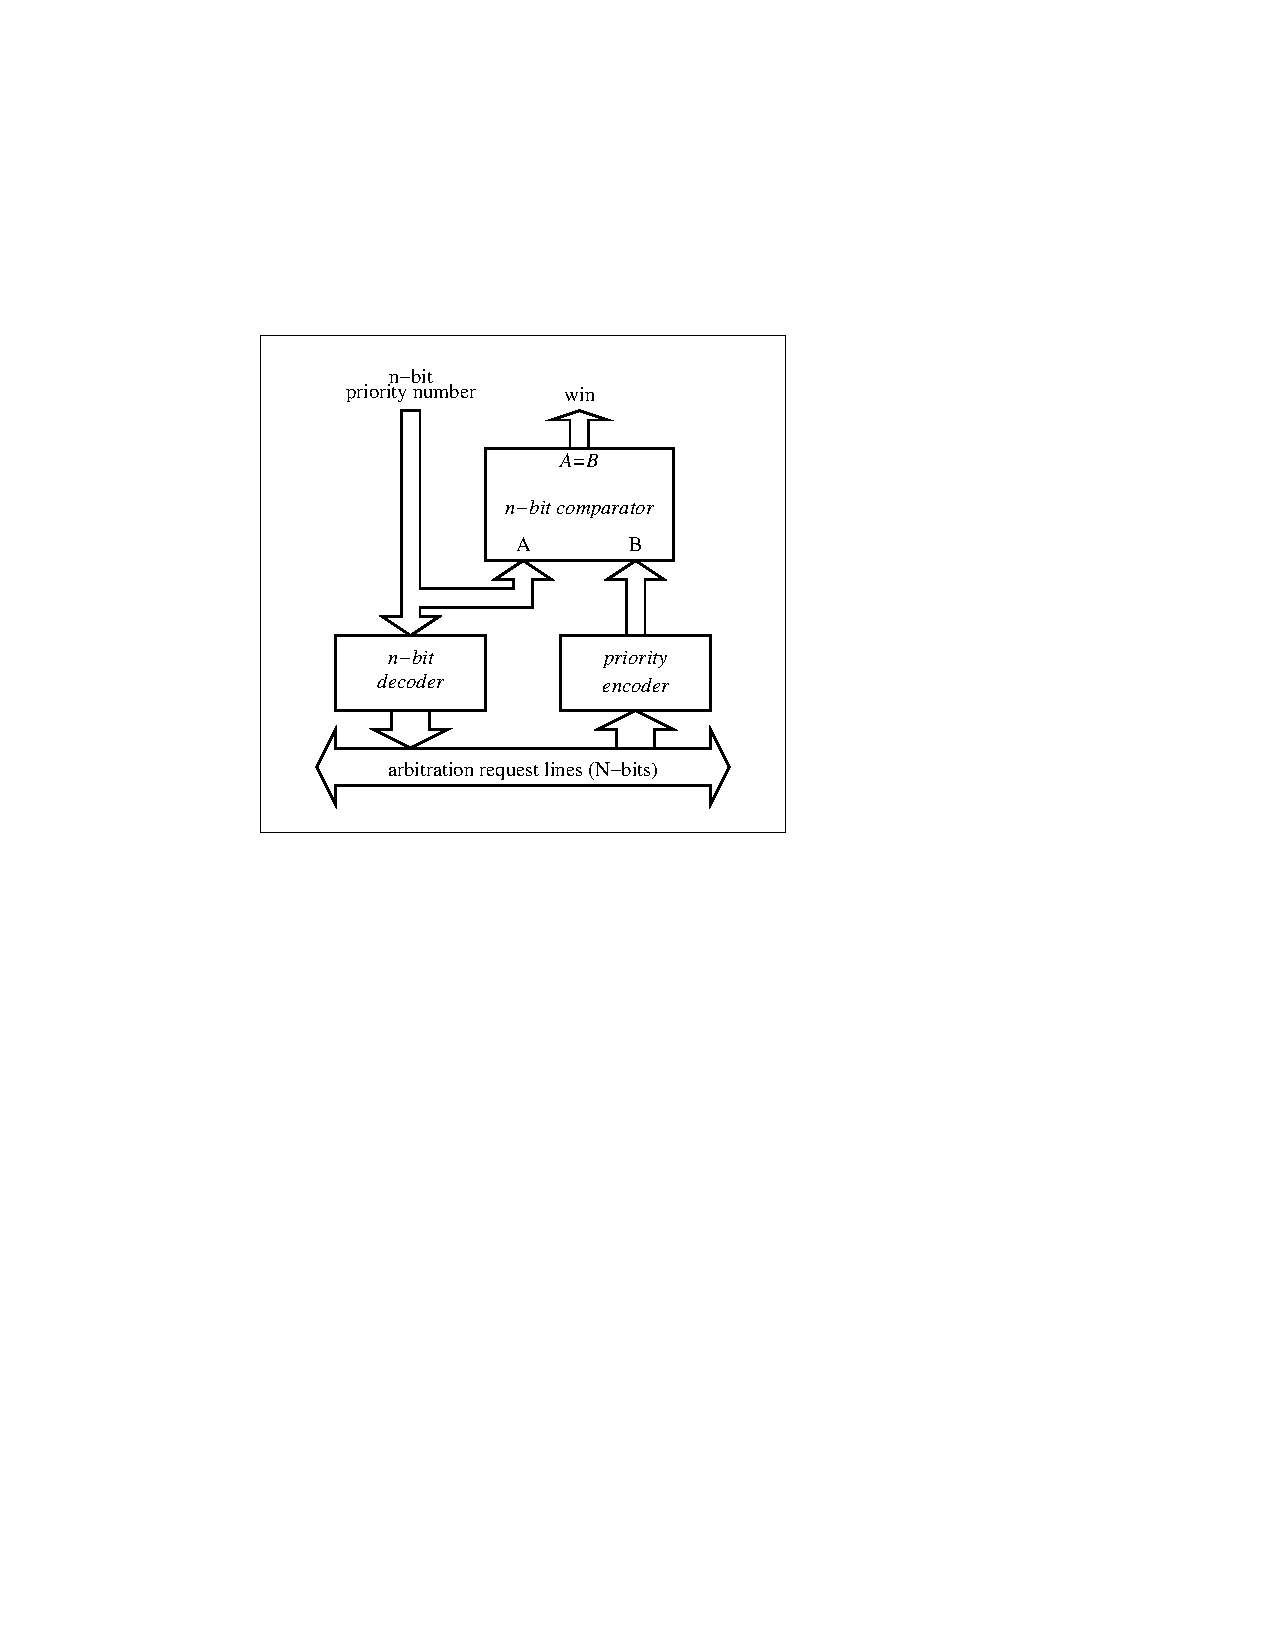
\includegraphics{ch2/FIG/arbiter.jpg}} %\centerline{\psfig{figure=ch2/FIG/arbiter.ps}}
   \caption{선형 자가 중재기의 일례}\label{figure:arbiter}
\end{figure}
중재는 버스 클럭을 기본단위로 하여 이루어진다. 즉 매 버스 클럭마다 한번의 중재가 이루어진다.
각 중재기에는 n-비트 우선순위(priority number)가 할당된다.
n-to-1 멀티플렉서(multiplexer)는 n-비트 우선순위 값을 입력으로 받아
이를 디코딩(decoding)하여
N-비트 폭의 신호선들 중 특정한 하나의 신호선을 구동한다.
이때 n과 N은 $n = \lceil \log_{2} N \rceil$\footnote{$\lceil x \rceil$ :
denotes the least integer that is greater than or equal to x.}의 관계에 있다.
우선순위 엔코더(priority encoder)는 N-비트 중재신호를 입력으로 받아
이들 중 가장 높은 우선순위를 갖는 신호의 번호를 엔코딩하여 출력한다.
비교기(comparator)는 미리 할당된 중재번호와 우선순위 엔코더에서 출력된 값을
비교하여 이들 둘이 같은지 여부를 출력한다.
따라서 비교기에서 출력이 있으면 해당 중재기가 현재 진행 중인 중재동작에서 가장 우선순위가
높은 것이므로 중재에서 이긴 것이 된다.
%
\subsection{공정성 규칙}
선형 자가 중재 방법은 기본적으로 우선 순위에 기초한 것이므로
우선순위가 높은 중재기가 상대적으로 자주 중재에서 이길 것이므로 균등한 중재 결과를 보장하기는 어렵다.
이러한 문제를 해결하기 위해서 가능한 균등하게 사용 기회를 제공하도록 하는 공정성 규칙(fairness rule)을
고려한다. \\
{\tt <}그림~\ref{figure:fairness}{\tt >}에 공정성 규칙을 나타내었다.
%\begin{figure}[htb]
%   \centerline{\psfig{figure=ch2/FIG/fairness.ps}}
%   \caption{공정성 중재 규칙}\label{figure:fairness}
%\end{figure}
%%%%%
%%Title: HiPi+Bus V0.2 Chapter 2
%%Creator: Ando Ki
%%CreationDate: April 1992
%%FileName: ch2
%%RelatedFile:
%%%%%
%\documentstyle[11pt,doublespace,a4wide,psfig]{hbook}
%\setstretch{1.2}
%\begin{document}
%
\begin{figure}[htb]
\begin{center}
  \begin{picture}(240,257)(-120,-257)
	\thicklines
	\put(0,-25){\circle{20}}
	\put(-45,-100){\framebox(90,45){}}
		\put(0,-70){\makebox(0,0){구동되어 있는}}
		\put(0,-82){\makebox(0,0){중재요청신호의}}
		\put(0,-94){\makebox(0,0){수를 계산한다}}
	\put(0,-120){\line(-5,-2){45}}
	\put(0,-120){\line(5,-2){45}}
	\put(0,-156){\line(-5,2){45}}
	\put(0,-156){\line(5,2){45}}
		\put(0,-138){\makebox(0,0){0 또는 1 ?}}
	\put(-91,-202){\framebox(72,36){}}
		\put(-55,-181){\makebox(0,0){다음 중재 싸이클}}
		\put(-55,-193){\makebox(0,0){까지 기다린다}}
	\put(19,-202){\framebox(72,36){}}
		\put(55,-181){\makebox(0,0){중재를}}
		\put(55,-193){\makebox(0,0){수행한다}}
	\put(55,-232){\circle{20}}
	\put(0,-35){\vector(0,-1){20}}
	\put(0,-100){\vector(0,-1){20}}
	\put(-45,-138){\line(-1,0){10}} \put(-55,-138){\vector(0,-1){28}}
		\put(-47,-136){\makebox(0,0)[rb]{아니오}}
	\put(45,-138){\line(1,0){10}} \put(55,-138){\vector(0,-1){28}}
		\put(47,-136){\makebox(0,0)[lb]{예}}
	\put(55,-202){\vector(0,-1){20}}
	\put(-45,-202){\line(0,-1){10}} \put(-45,-212){\line(-1,0){56}}
		\put(-101,-212){\line(0,1){167}} \put(-101,-45){\vector(1,0){101}}
	\put(-120,-257){\framebox(240,257){}} % 외곽 box
  \end{picture}
\end{center}
  \caption{공정성 중재 규칙}\label{figure:fairness}
\end{figure}
%%%%
%\end{document}
%%%%

중재가 버스 클럭을 기본단위로 이루어지므로 공정성 규칙도 버스 클럭 단위로 이루어진다.
중재에 참가하기에 앞서 현재 중재에 참가하고 있는 중재기의 갯수를 파악한다.
이것은 중재 버스에 현재 구동되어 있는 중재 요청 신호의 갯수를 알아내는 것으로 가능하다.
그 갯수가 두개 이상이면 현재 중재에 참가 중인 중재기가 두개 이상이라는 것을 의미하고
이어지는 버스 클럭에는 현재 진행 중인 중재에서 이기지 못한 중재 요청이 한개 또는 그 이상
남아 있을 것이 확실하므로 곧 바로 중재에 참가하지 않고 또 다시 공정성 규칙에 따라 점검을 한다.
그러나 만약 그 갯수가 한개 또는 없음이 확인되는 경우는 이어지는 버스 클럭에는
현재 진행 중인 중재에서 이기지 못한 중재기가 없을 것이 확실하므로
곧 바로 중재에 참가한다. 이러한 중재 규칙은 시간적으로 우선하여 발생한 중재 요청은
항상 먼저 처리됨을 보장하게 된다.
%
%

\newpage
%%%%%
%%Title: HiPi+Bus V0.2 Chapter 2 sec 4
%%Creator: Ando Ki
%%CreationDate: April 1992
%%FileName: sec4
%%RelatedFile: ch2
%%%%%
\section{어드레스 버스 중재}
어드레스 버스 중재(address bus arbitration)는
어드레스 기본 사이클(address basic cycle)과
어드레스 데이터 기본 사이클(address data basic cycle)에 앞서 항상 수행해야 된다.
어드레스 버스 중재는 선형 자가 중재 기법을 사용하며 공정성 규칙을 지켜야 한다.
그러나 재시도(retry)하는 경우는 공정성 규칙을 무시한다.
ABINH* 신호가 구동되어 있는 동안은 중재를 수행하지 않거나 중재의 결과를 무시하여야 한다.
WRINH* 신호가 구동되어 있는 동안은 쓰기에 관련된 전송의
중재를 수행하지 않거나 중재의 결과를 무시하여야 한다. \\
일정시간 이상 메모리 참조에 실패한 경우 ABINH* 신호를 구동할 수 있다.
%

\newpage
%%%%%
%%Title: HiPi+Bus V0.1 Chapter 2 sec 5
%%Creator: Ando Ki
%%CreationDate: April 1992
%%FileName: sec5
%%RelatedFile: ch2
%%%%%
\section{데이터 버스 중재}
데이터 버스 중재(data bus arbitration)는
데이터 기본 사이클(data basic cycle)에 앞서 항상 수행해야 된다.
데이터 버스 중재는 선형 자가 중재 기법을 사용한다.
데이터 버스 중재는 공정성 규칙을 지켜야 하며 이 공정성 규칙은 시간적으로
우선하여 발생한 요청을 먼저 처리할 수 있도록 한다.
DBINH* 신호가 구동되어 있는 동안은 중재를 수행하지 않거나,
중재의 결과를 무시하여야 한다.
이것은 쓰기에 관련된 전송에서 구동하는 데이터와 데이터 버스 중재의 결과에 의해
구동하는 데이터가 충돌하는 것을 방지하기 위해서이다. \\
일정시간 이상 데이터 중재에 실패하는 경우 ABINH* 신호를 구동할 수 있다. \\
PCW* 신호가 구동되어 있는 것이 확인 된 경우 확인 된 다음 사이클 부터
PCW* 신호가 걷어진 그 다음 사이클 까지 데이터 버스 중재 동작에
참여하여서는 안된다. 즉 DBRQ{\tt <}n{\tt >}* 신호와
WRINH* 신호를 구동하여서는 안된다.
%

%%%%%

%%%%%
%%Title: HiPi+Bus V0.2 Chapter 3
%%Creator: Ando Ki
%%CreationDate: April 1992
%%FileName: ch3
%%RelatedFile: sec1 sec2
%%%%%
\chapter{데이터 전송 버스}
%
%%%%%
%%Title: HiPi+Bus V0.2 Chapter 3 Section 1
%%Creator: Ando Ki
%%CreationDate: April 1992
%%FileName: sec1
%%RelatedFile: ch3
%%%%%
%\documentstyle[doublespace,a4wide]{hbook}
%\setstretch{1.2}
%\pagestyle{headings}
%\begin{document}
%\pagenumbering{arabic}
%\setcounter{chapter}{1}
%
\section{개요}
데이터 전송 버스(data transfer bus : DTB)는 데이터의 전송에 직접적으로 관련되는 신호선의 모임이며,
어드레스 버스(address bus : AB), 데이터 버스(data bus : DB),
그리고 상태 버스(status bus : SB)로 구성된다.
%
\begin{table}[htbp]
\caption{데이터 전송 버스의 규격 요약}\label{table:dtb-spec}
   \begin{center}
\begingroup
\setlength{\tabcolsep}{6pt} % Default value: 6pt
\renewcommand{\arraystretch}{0.9} % Default value: 1
   \begin{tabular}{|l l|} \hline
      \multicolumn{2}{|c|}{데이터 전송 프로토콜 (Data Transfer Protocols)} \\ \hline
      Protocol & Pended \\
      제어 방식 & 동기형 (Synchronous) \\
      클럭의 속도 & 16.5 MHz (60.6 {\it n\/}sec) \\
      데이터 전송 속도(Data Bandwidth) & 264 Mbytes/sec\\ \hline
      \multicolumn{2}{|c|}{어드레스 버스의 특성 (Characteristics of Address Bus)} \\ \hline
      최대 어드레스 영역의 크기 & 4 Gbytes \\
      어드레스 영역의 갯수 & 8 \\
      최대 사용 가능한 전송 형태 & 32 \\ \hline
      \multicolumn{2}{|c|}{데이터 버스의 특성 (Characteristics of Data Bus)} \\ \hline
      버스의 폭 (Bus Width) & 128 bits (16 bytes) \\
      데이터의 단위 (Data Unit) & 8 bits (1 byte) \\
      전송 가능한 데이터의 크기 & 16-바이트 이내의 연속된 바이트; 64-바이트 \\
      정렬의 제약 (Alignment Restriction) & 16 byte boundary; 64 byte boundary \\
      Justification & Straight (Nonjustified) \\ \hline
      \multicolumn{2}{|c|}{에러 방어 (Error Protection)} \\ \hline
      에러 검출 (Error Detection) & 바이트 단위의 홀수 패리티 (odd parity) \\
      에러의 처리 (Error Handling) & 재시도 (Retry) \\ \hline
      \multicolumn{2}{|c|}{기 타 (Etc.)} \\ \hline
      캐쉬 지원 & Write Back \\
      동기화 지원 (Synchronization) & Semaphore Cache Protocol \\
      총 신호수 & 244\\ \hline
   \end{tabular}
\endgroup
   \end{center}
\end{table}
%

%
%%%%%
%\end{document}
%%%%%

\newpage
%%%%
%%Title: HiPi+Bus V0.2 Chapter 3
%%Creator: Ando Ki
%%CreationDate: April 1992
%%FileName: sec2
%%RelatedFile: ch3
%%%%%
%%%%%
%\documentstyle[doublespace,a4wide]{hbook}
%\setstretch{1.2}
%\pagestyle{headings}
%\begin{document}
%\pagenumbering{arabic}
%\setcounter{chapter}{1}
%
\section{데이터 전송 버스의 신호선}
%\documentstyle[a4]{hbook}
%\begin{document}
%
\begin{table}[htbp]
\caption{데이터 전송 버스의 신호선 요약}
   \begin{center}
   \begin{tabular}{|l|r|l|} \hline
      Mnemonics & size & name \\ \hline \hline
      \multicolumn{3}{|c|}{Address Bus} \\ \hline
      A{\tt <}31..4{\tt >}*  & 28 & Address \\
      AP{\tt <}3..0{\tt >}*  & 4 & Address Parity \\
      SI{\tt <}7..0{\tt >}*  & 8 & Source Identification \\
      SIP*                   & 1 & Source Identification Parity \\
      AS{\tt <}2..0{\tt >}*  & 3 & Address Space \\
      TT{\tt <}4..0{\tt >}*  & 5 & Transfer Types \\
      STP*                   & 1 & Space + Types Parity \\
      BE{\tt <}15..0{\tt >}* & 16 & Byte Enable \\
      BEP{\tt <}1..0{\tt >}* & 2 & Byte Enable Parity \\
      AE*                    & 1 & Address Bus Enable \\ \hline
      \multicolumn{3}{|c|}{Data Bus} \\ \hline
      D{\tt <}127..0{\tt >}* & 128 & Data \\
      DP{\tt <}15..0{\tt >}* & 16 & Data Parity \\
      DI{\tt <}7..0{\tt >}*  & 8 & Destination Identification \\
      DIP*                   & 1 & Destination Identification Parity \\
      DE*                    & 1 & Data Bus Enable \\ \hline
      \multicolumn{3}{|c|}{Status Bus} \\ \hline
      AACK{\tt <}1..0{\tt >}* & 2 & Address Acknowledge \\
      SHD*                    & 1 & Hit on Shared Line \\
      DTY*                    & 1 & Hit on Dirty Block \\
      SNK*                    & 1 & Snoop No Acknowledge \\
      ITV*                    & 1 & Intervention \\
      LCR*                    & 1 & Hit On Interlocked Region \\
      SPIN{\tt <}3..0{\tt >}* & 4 & Spin Queue Order \\
      DACK*                   & 1 & Data Acknowledge \\
      CDK*                    & 1 & Cache Data Acknowledge \\
      BSY{\tt <}7..0{\tt >}* & 8 & Busy Status Line \\ \hline
   \end{tabular}
   \end{center}
\end{table}
%
%\end{document}

\subsection{어드레스 버스의 신호선 (signal lines of address bus)}
어드레스 버스는 어드레스, 어드레스 영역, 전송의 종류, 전송하고자 하는 데이터의 크기, 어드레스를
구동하는 모듈의 식별자, 각 신호의 패리티, 그리고 어드레스 버스가 구동되고 있음을 알리는 제어신호로
구성된다.
%
\subsubsection{Address : A$<$31..4$>$*}
전송할 데이터의 위치를 알리는 주소이다. 32 비트 중 A$<$31$>$*이
가장 높은 자리수이다.
A$<$3..0$>$* 4개 비트가 없는 대신
16 바이트 이내의 유효 데이터는 BE$<$15..0$>$*에 의해
식별된다.
%
\subsubsection{Address Parity : AP$<$3..0$>$*}
어드레스 신호선의 각 바이트에 해당하는 패리티이다.
AP$<$0$>$*값은 A$<$3..0$>$*의 값을
0x0으로 간주한 상태에서 계산된 값이다.
%\documentstyle[a4]{hbook}
%\begin{document}
%
\begin{table}[htbp]
\caption{어드레스와 패리티 비트}
   \begin{center}
   \begin{tabular}{|l|l||l|l|} \hline
      address & address parity & address & address parity \\ \hline \hline
      A{\tt <}31..24{\tt >}* & AP{\tt <}3{\tt >}* &
      A{\tt <}23..16{\tt >}* & AP{\tt <}2{\tt >}* \\ \hline
      A{\tt <}15..8{\tt >}* & AP{\tt <}1{\tt >}* &
      A{\tt <}7..0{\tt >}* & AP{\tt <}0{\tt >}* \\ \hline
   \end{tabular}
   \end{center}
\end{table}
%
%\end{document}

%
\subsubsection{Source Identification : SI$<$7..0$>$*}
어드레스의 구동에 의해서 버스 동작이 시작되며 이 버스 동작은 데이터를 요청하거나 쓰거나 한다.
이때 어드레스 구동과 같은 시간에 해당 SI$<$7..0$>$*를 구동하여 버스 동작을 시작한 모듈을
알린다. 비트 5 - 2에 채워지는 슬롯 어드레스는 해당 슬롯의 GA$<$3..0$>$* 값이고,
비트 1 - 0에 채워지는 값은 해당 보드 내에서 정의한다.
%\documentstyle[a4]{hbook}
%\begin{document}
%
\begin{table}[htbp]
\caption{시발점 식별자}
   \begin{center}
   \begin{tabular}{|l|l|} \hline
      field & meaning \\ \hline \hline
      SI{\tt <}7..6{\tt >}* & {\it reserved\/} \\ \hline
      SI{\tt <}5..2{\tt >}* & slot address \\ \hline
      SI{\tt <}1..0{\tt >}* & channel identification \\ \hline
   \end{tabular}
   \end{center}
\end{table}
%
%\end{document}

%
\subsubsection{Source Identification Parity : SIP*}
SI$<$7..0$>$*의 패리티 비트이다.
%
\subsubsection{Address Space : AS$<$2..0$>$*}
어드레스 영역을 구분하기 위한 신호이며 3비트의 신호로 8개의 독립적인 어드레스 영역을 사용할 수 있지만
현재 정의하여 사용하는 것은 메모리 영역, 입출력 영역, 그리고 시스템 영역이고 나머지는 확장을 위해 사용을 유보한다.
각 어드레스 영역은 4GBytes의 크기를 갖는다.
%\documentstyle[a4]{hbook}
%\begin{document}
%
\begin{table}[htbp]
\caption{정의된 어드레스 영역}
   \begin{center}
   \begin{tabular}{|l|l|l|l|} \hline
      AS{\tt <}2..0{\tt >}* & name & size & application \\ \hline \hline
      0x0 & memory space & 4GBytes & shared memory \\ \hline
      0x3 & input/output space & 4GBytes & memory mapped peripherals\\ \hline
      0x7 & system space & 4GBytes & system configuration registers\\ \hline
   \end{tabular}
   \end{center}
\end{table}
%
%\end{document}

%
\subsubsection{Transfer Types : TT$<$4..0$>$*}
전송의 종류를 정의하는 신호이다. \\
정의된 데이터 전송은 데이터의 이동 방향에 따라
읽기 전송, 쓰기 전송, 그리고 어드레스 단일 전송으로 구분된다.
읽기 전송은 데이터가 RP에서 RQ로 공급되며, 쓰기 전송은 데이터가 RQ에서 RP로 
공급된다.
어드레스 단일 전송은 데이터의 이동이 없다. \\
각 전송은 이동되는 데이터의 크기에 따라 단일 전송과 블록 전송으로 구분된다.
단일 전송의 경우는 16바이트 경계로 정렬된 어드레스(어드레스를 16로 나누어 나머지가 없는 경우)에서
1-바이트, 또는 연속된 16-바이트 이내의 데이터를 BE$<$15..0$>$*로
지정하여 전송가능하다.
블록 전송의 경우는 64바이트 경계로 정렬된 어드레스(어드레스를 64로 나누어 나머지가 없는 
경우)에서부터 64바이트를 전송가능하다. 이때 BE$<$15..0$>$*는 0xFF로 구동한다.
참고로, 
TT$<$4$>$*는 블록 전송을, TT$<$3$>$*은 쓰기 전송임을 나타낸다.

%\documentstyle[a4]{hbook}
%\begin{document}
%
\begin{table}[htbp]
\caption{전송 형태}
   \begin{center}
   \begin{tabular}{|l|l|l|l|l|l|} \hline
      TT{\tt <}4..0{\tt >}* & mnemonics & name & group & affect cache & size \\ \hline \hline
      0x00 & NRD & normal read        & read  & yes & 1--16 \\ \hline
      0x08 & NWR & normal write       & write & yes & 1--16 \\ \hline
      0x07 & NCR & non-coherent read  & read  & no  & 1--16 \\ \hline
      0x0F & NCW & non-coherent write & write & no  & 1--16 \\ \hline
      0x03 & IVD & invalidation       &       & yes & \\ \hline
      0x04 & ILR & interlock read     & read  & yes & 1--16 \\ \hline
      0x0C & ILW & interlock write    & write & yes & 1--16 \\ \hline
      0x10 & BRD & block read         & read  & yes & 64 \\ \hline
      0x18 & BWR & block write        & write & yes & 64 \\ \hline
      0x12 & CRD & coherent read      & read  & yes & 64 \\ \hline
      0x11 & EXR & exclusive read     & read  & yes & 64 \\ \hline
      0x19 & WRB & writeback          & write & yes & 64 \\ \hline
      0x1B & ITW & intervention write & write & yes & 64 \\ \hline
   \end{tabular}
   \end{center}
\end{table}
%
%\end{document}

\begin{itemize}
	\item Normal Read : NRD \\
	단일 전송에 속하며,
	단순히 RP로부터 원하는 데이터를 읽어온다. 이때 해당 데이터는 캐쉬에 저장되지 않는다.
	\item Normal Write : NWR \\
	단일 전송에 속하며,
	단순히 RP로 특정 데이터를 쓴다.
	\item Non-Coherent Read : NCR \\
	단일 전송에 속하며,
	단순히 RP로부터 원하는 데이터를 읽어온다.
	캐쉬 동일성 유지 프로토콜과 전혀 관련이 없는 데이터가 읽혀질 때 사용된다.
	따라서 시스템 내의 모든 캐쉬는 이 전송에 대하여 아무 것도 고려할 것이 없다.
	\item Non-Coherent Write : NCW \\
	단일 전송에 속하며,
	단순히 RP로 특정 데이터를 쓰는 동작으로
	캐쉬 동일성 유지 프로토콜과 전혀 관련이 없는 특정 데이터를 쓸 때 사용한다.
	따라서 시스템 내의 모든 캐쉬는 이 전송에 대하여 아무 것도 고려할 것이 없다.
	\item Invalidation : IVD \\
	어드레스 단일 전송에 속하며,
	캐쉬 동일성 유지 프로토콜을 유지할 책임이 있는 RQ가 자신의 캐쉬에 있는 유효 데이터를
	시스템을 통하여 유일한 유효 데이터로 만들기 위해 캐쉬 동일성 유지 프로토콜을 
	유지할 책임이 있는 다른 RQ들에게 알릴 때 사용한다.
	즉, 다른 캐쉬에 있는 동일 데이터를 무효화시킬 때 사용한다.
	이 전송은 어드레스 기본 사이클만으로 수행된다.
	특히 IVD의 경우 AACK$<$1..0$>$*는 의미를 갖지 않고 대신 SNK*이 사용된다.
	\item Interlock Read : ILR \\
	단일 전송에 속하며,
	잠금동작을 위한 전송으로 이 전송에 의해 잠금이 시작된다.
	NRD와 동일한 버스동작으로 수행되지만 이 전송이 완료된 이후는 해당 영역이 잠금상태가 된다.
	\item Interlock Write : ILW \\
	단일 전송에 속하며,
	잠금동작을 위한 전송으로 이 전송에 의해 잠금이 풀린다.
	NWR와 동일한 버스동작으로 수행되지만 이 전송이 완료된 이후는 해당 영역이 잠금상태에서 풀린다.
	\item Block Read : BRD \\
	블록 전송에 속하며,
	단순히 RP로부터 원하는 데이터를 읽어오며, 이때 해당 데이터는 캐쉬에 저장되지 않는다.
	\item Block Write : BWR \\
	블록 전송에 속하며,
	단순히 RP로 특정 데이터를 쓴다.
	\item Coherent Read : CRD \\
	블록 전송에 속하며,
	캐쉬 동일성 유지 프로토콜을 유지할 책임이 있는 RQ가 데이터를 읽을 때 사용되며,
	읽혀진 데이터가 RQ내의 캐쉬에 저장되어 사용된다. 이때 그 데이타가 전체 시스템을 통하여 유일한
	유효 데이터일 필요는 없다.
	\item Exclusive Read : EXR \\
	블록 전송에 속하며,
	캐쉬 동일성 유지 프로토콜을 유지할 책임이 있는 RQ가 데이터를 읽을 때 사용되며,
	읽혀진 해당 데이터는 전체 시스템을 통하여 유일한 유효 데이터이여야 한다.
	\item Writeback : WRB \\
	블록 전송에 속하며,
	캐쉬 동일성 유지 프로토콜을 유지할 책임이 있는 RQ가 자신의 캐쉬에 있는 유일한 유효 데이터를
	메모리로 또는 메모리와 다른 RQ로 전달할 때 사용한다.
	이때 DI*가 실제 데이터의 종착지를 결정한다. (주의: RQ에서 RQ로만
	데이터가 전달될 때는 ITW를 사용해야만 한다.)
	\item Intervention Write : ITW \\
	블록 전송에 속하며,
	캐쉬 동일성 유지 프로토콜을 유지할 책임이 있는 RQ가 자신의 캐쉬에 있는 유효 데이터를
	다른 특정 RQ에 전달할때 사용한다. 이 전송은 인터벤션이 선행되는 전송이다.
	특히 ITW의 경우 AACK$<$1..0$>$*는 의미를 갖지 않고,
	대신 SNK*가 사용되며, DACK*는 의미를 갖지 않고 CDK*가 사용된다.
\end{itemize}
%
\subsubsection{Address Space and Transfer Types Parity : STP*}
AS$<$2..0$>$*와 TT$<$4..0$>$*를 합한 8 비트에 대한 패리티 비트이다.
%
\subsubsection{Byte Enable : BE$<$15..0$>$*}
단일 전송(NRD, NWR, NCR, NCW, ILR, ILW)때만 유효하며,
1에서 16까지의 연속된 데이터를 지정하는 신호이다.
16 비트의 신호는 데이터 버스의 각 바이트에 대응한다.
블록 전송의 경우 0xFF로 구동한다.
%\documentstyle[a4]{hbook}
%\begin{document}
%
\begin{table}[htbp]
\caption{바이트 지정자}
   \begin{center}
   \begin{tabular}{|l|l||l|l|} \hline
      data bus & byte enable bit & data bus & byte enable bit \\ \hline \hline
      D{\tt <}127..120{\tt >}* & BE{\tt <}15{\tt >}* &
      D{\tt <}63..56{\tt >}* & BE{\tt <}7{\tt >}* \\ \hline
      D{\tt <}119..112{\tt >}* & BE{\tt <}14{\tt >}* &
      D{\tt <}55..48{\tt >}* & BE{\tt <}6{\tt >}* \\ \hline
      D{\tt <}111..104{\tt >}* & BE{\tt <}13{\tt >}* &
      D{\tt <}47..40{\tt >}* & BE{\tt <}5{\tt >}* \\ \hline
      D{\tt <}103..96{\tt >}* & BE{\tt <}12{\tt >}* &
      D{\tt <}39..32{\tt >}* & BE{\tt <}4{\tt >}* \\ \hline
      D{\tt <}95..88{\tt >}* & BE{\tt <}11{\tt >}* &
      D{\tt <}31..24{\tt >}* & BE{\tt <}3{\tt >}* \\ \hline
      D{\tt <}87..80{\tt >}* & BE{\tt <}10{\tt >}* &
      D{\tt <}23..16{\tt >}* & BE{\tt <}2{\tt >}* \\ \hline
      D{\tt <}79..72{\tt >}* & BE{\tt <}9{\tt >}* &
      D{\tt <}15..8{\tt >}* & BE{\tt <}1{\tt >}* \\ \hline
      D{\tt <}71..64{\tt >}* & BE{\tt <}8{\tt >}* &
      D{\tt <}7..0{\tt >}* & BE{\tt <}0{\tt >}* \\ \hline
   \end{tabular}
   \end{center}
\end{table}
%
%\end{document}

%
\subsubsection{Byte Enable Parity : BEP$<$1..0$>$*}
BE$<$15..0$>$*에 대한 패리티 비트이다.
%\documentstyle[a4]{hbook}
%\begin{document}
%
\begin{table}[htbp]
\caption{바이트 지정자와 패리티 비트}
   \begin{center}
   \begin{tabular}{|l|l||l|l|} \hline
      byte enable & byte enable parity & byte enable & byte enable parity \\ \hline \hline
      BE{\tt <}15..8{\tt >}* & BEP{\tt <}1{\tt >}* &
      BE{\tt <}7..0{\tt >}* & BEP{\tt <}0{\tt >}* \\ \hline
   \end{tabular}
   \end{center}
\end{table}
%
%\end{document}

%
\subsubsection{Address Bus Enable : AE*}
현재 진행 중인 주기에서 어드레스 버스의 신호들이 유효한 값을 갖는다는 것을 나타낸다.
%
\subsection{데이터 버스의 신호선 (signal lines of data bus)}
데이터 버스는 데이터, 해당 데이터가 도착해야 하는 모듈(들)의 식별자,
각 신호의 패리티, 그리고 데이터 버스가 구동되고 있음을 알리는 제어신호로
구성된다.
\subsubsection{Data : D$<$127..0$>$*}
128 비트 (16 바이트) 폭의 데이터 신호선이다.
%
\subsubsection{Data Parity : DP$<$15..0$>$*}
데이터 신호선의 각 바이트에 해당하는 패리티이다. 16 바이트 이내의 데이터를
전송할 때 BE$<$15..0$>$*에 의해 지정된 유효한 바이트에 대응하는 패리티는
반드시 정확한 패리티 값을 가져야하고 나머지는 상관하지 않아도 된다.
그러나 가능한 모든 바이트의 패리티가 정확한 값을 갖는 것이 좋다.
%\documentstyle[a4]{hbook}
%\begin{document}
%
\begin{table}[htbp]
\caption{데이터와 데이터 패리티}
   \begin{center}
   \begin{tabular}{|l|l||l|l|} \hline
      data bus & data parity bit & data bus & data parity bit \\ \hline \hline
      D{\tt <}127..120{\tt >}* & DP{\tt <}15{\tt >}* &
      D{\tt <}63..56{\tt >}* & DP{\tt <}7{\tt >}* \\ \hline
      D{\tt <}119..112{\tt >}* & DP{\tt <}14{\tt >}* &
      D{\tt <}55..48{\tt >}* & DP{\tt <}6{\tt >}* \\ \hline
      D{\tt <}111..104{\tt >}* & DP{\tt <}13{\tt >}* &
      D{\tt <}47..40{\tt >}* & DP{\tt <}5{\tt >}* \\ \hline
      D{\tt <}103..96{\tt >}* & DP{\tt <}12{\tt >}* &
      D{\tt <}39..32{\tt >}* & DP{\tt <}4{\tt >}* \\ \hline
      D{\tt <}95..88{\tt >}* & DP{\tt <}11{\tt >}* &
      D{\tt <}31..24{\tt >}* & DP{\tt <}3{\tt >}* \\ \hline
      D{\tt <}87..80{\tt >}* & DP{\tt <}10{\tt >}* &
      D{\tt <}23..16{\tt >}* & DP{\tt <}2{\tt >}* \\ \hline
      D{\tt <}79..72{\tt >}* & DP{\tt <}9{\tt >}* &
      D{\tt <}15..8{\tt >}* & DP{\tt <}1{\tt >}* \\ \hline
      D{\tt <}71..64{\tt >}* & DP{\tt <}8{\tt >}* &
      D{\tt <}7..0{\tt >}* & DP{\tt <}0{\tt >}* \\ \hline
   \end{tabular}
   \end{center}
\end{table}
%
%\end{document}

%
\subsubsection{Destination Identification : DI$<$7..0$>$*}
데이터 버스에 구동되고 있는 데이터가 실제로 어디로 이동하는 것인지를 알리기 위해 사용된다.
메모리 모듈만 지정되는 경우는 RQ에 의해 메모리 쓰기가 수행될 때 사용하며,
이때 비트 5 - 0의 값은 데이터를 구동하는 RQ를 구별하는 정보이다.
특정 RQ만 지정되는 경우는 메모리 읽기에 대한 데이터 응답이나
캐쉬에서 캐쉬로 데이터 이동이 필요할 때 사용하며,
이때 비트 5 - 0의 값은 데이터를 받을 RQ를 구별하는 정보이다.
RQ와 RP가 동시에 지정되는 경우는
비트 7 - 6의 값이 0x3이고 비트 5 - 0의 값은 데이터를 받을 특정 RQ를 구별하는
정보이다.
%\documentstyle[a4]{hbook}
%\begin{document}
%
\begin{table}[htbp]
\caption{종착점 식별자}
   \begin{center}
   \begin{tabular}{|l|l|l||l|} \hline
      DI$<$7..6$>$* & DI$<$5..2$>$* & DI$<$1..0$>$* & meaning \\ \hline \hline
      00 & {\it reserved\/} & {\it reserved\/} & {\it reserved\/} \\ \hline
      01 & slot address     & channel id.      & to RQ only \\ \hline
      l0 & slot address     & channel id.      & to RP only \\ \hline
      11 & slot address     & channel id.      & to RQ and RP \\ \hline
   \end{tabular}
   \end{center}
\end{table}
%
%\end{document}

%
\subsubsection{Destination Identification Parity : DIP*}
DI$<$7..0$>$*의 패리티 비트이다.
%
\subsubsection{Data Bus Enable : DE*}
현재 진행 중인 주기에서 데이터 버스의 신호들이 유효한 값을 갖는다는 것을 나타낸다.
%
\subsection{상태 버스의 신호선 (signal lines of status bus)}
상태 버스는 어드레스 전달에 대한 응답, 데이터 전달에 대한 응답, 그리고 캐쉬 동일성 유지
프로토콜에 필요한 제어 신호, 잠금에 대한 응답 신호로 구성된다.
%
\subsubsection{Address Acknowledge : AACK$<$1..0$>$*}
어드레스 전달에 대해 어드레스를 받은 모듈이 그 상태를 알리는 신호이다.
%\documentstyle[a4]{hbook}
%\begin{document}
%
\begin{table}[htbp]
\caption{어드레스 응답}
   \begin{center}
   \begin{tabular}{|l|l|l|} \hline
      AACK$<$1..0$>$* & status & description \\ \hline \hline
      00 & error & 전송된 어드레스 버스의 정보에 오류가 발견됨 \\ \hline
      01 & busy & 전송된 어드레스 버스의 정보를 현재 받을 수 없는 상태임 \\ \hline
      10 & lock & 요청한 영역이 잠겨 있음 \\ \hline
      11 & no error & 전송된 어드레스 버스의 정보를 잘 받았음 \\ \hline
   \end{tabular}
   \end{center}
\end{table}
%
%\end{document}

%
\subsubsection{Hit On Shared Line : SHD*}
$RQ_1$에 의해 진행되는 버스 동작에 의해 요청되는 데이터의 유효한 내용을 
자신의 캐쉬에 갖는 $RQ_2$는 SHD* 신호선을 구동하여 $RQ_1$으로하여금
요청되는 데이터가 다른 캐쉬에도 있음을 알린다.
SHD*는 진행 중인 데이터 전송에 아무런 영향을 주지 않으며
단지 다른 캐쉬에 공유되고 있음을 알리는 신호이다.
%\documentstyle[a4]{hbook}
%\begin{document}
%
\begin{table}[htbp]
\caption{SHD*}\label{tbl:shd}
   \begin{center}
   \begin{tabular}{|c|l|} \hline
      SHD* & description \\ \hline \hline
      0    & - \\ \hline
      1    & hit on shared line \\ \hline
   \end{tabular}
   \end{center}
\end{table}
%
%\end{document}

%
\subsubsection{Hit On Dirty Line : DTY*}
$RQ_1$에 의해 진행되는 버스 동작에 의해 요청되는 데이터의 유효한 값이 메모리에 있지 않고
$RQ_2$의 캐쉬에 있을 때,
자신의 캐쉬에 유일한 유효 데이터를 갖는 $RQ_2$는 DTY* 신호선을 구동하여
$RQ_1$의 진행 중인 데이터 전송을 중지시키고 메모리의 데이터 응답을 방지한다. \\
DTY* 신호가 구동되면 해당 데이터 전송을 수행하는 RQ는 재시도를 해야하고
메모리는 데이터 응답을 하지 않아야 한다.
그리고 DTY* 신호를 구동한 RQ는 자신의 유일한 유효 데이터를 메모리에
반영할 의무를 진다.
%\documentstyle[a4]{hbook}
%\begin{document}
%
\begin{table}[htbp]
\caption{DTY*}\label{tbl:dty}
   \begin{center}
   \begin{tabular}{|c|l|} \hline
      DTY* & description \\ \hline \hline
      0    & - \\ \hline
      1    & hit on dirty line \\ \hline
   \end{tabular}
   \end{center}
\end{table}
%
%\end{document}

%
\subsubsection{Intervention : ITV*}
$RQ_1$에 의해 진행되는 버스 동작에 의해 요청되는 데이터의 유효한 값이 메모리에 있지 않고
$RQ_2$의 캐쉬에 있을 때,
$RQ_2$는 ITV* 신호선을 구동하여 메모리의 데이터
응답을 방지하고 자신이 가지고 있는 유효한 데이터를 $RQ_1$에 공급할 수 있다.
그러나 데이터를 요구한 $RQ_1$은 버스 동작을 계속 진행해야 한다.

ITV* 신호를 구동한 $RQ_2$는 ITW 전송으로
자신의 유일한 유효 데이터를 해당 데이터를 요청한 $RQ_1$에게 전달하거나,
WRB 전송으로 $RQ_1$과 메모리에 동시에 반영할 수 있다.
ITV* 신호에 의해 인터벤션 상태에 있는 $RQ_1$은 전달받은 데이터에 대한 DACK* 대신
CDK*로써 응답한다. 만약 CDK*로 에러의 발생을 알린 경우, ITV* 신호를 받은 $RQ_1$은 요청을
재시도하며, ITV* 신호를 구동했던 $RQ_2$는 전송을 다시 시도하지 않는다.
그러나 $RQ_1$이 CDK*를 오류로 구동했으므로 재시도 할 것이고,
이것에 의해 다시 $RQ_2$가 적절한 동작을 할 수 있다.

이 신호는 캐쉬 동일성 유지 프로토콜을 유지할 책임이 있는 RQ가 현재 요청되는
데이터를 자신의 캐쉬에서 공급하고자 할 때 사용한다. 이 신호가 구동되면 메모리는 데이터를
응답하지 말아야 하며, 이 신호를 구동한 RQ는 반드시 해당 데이터를 공급할 의무를 진다.
%\documentstyle[a4]{hbook}
%\begin{document}
%
\begin{table}[htbp]
\caption{ITV*}\label{tbl:itv}
   \begin{center}
   \begin{tabular}{|c|l|} \hline
      ITV* & description \\ \hline \hline
      0    & - \\ \hline
      1    & intervention \\ \hline
   \end{tabular}
   \end{center}
\end{table}
%
%\end{document}

%
\subsubsection{Snoop No Acknowledge : SNK*}
캐쉬 동일성 유지 프로토콜을 유지할 책임이 있는 $RQ_1$이 현재 진행 중인
버스 동작이 자신의 캐쉬에 영향을 주는 것인데도 불구하고 자신이 이에 합당한 캐쉬 동작을
할 수 없거나 또는 진행 중인 버스 동작에 관련된 자신의 캐쉬 동작에 문제가 발생한 경우
해당 버스 동작을 더 이상 진행되지 못하도록 하기 위해 구동한다.
SNK* 신호가 구동되면 해당 데이터 전송을 수행하는 $RQ_2$는 재시도를 해야하고
메모리는 데이터 응답을 하지 않아야 한다.
%\documentstyle[a4]{hbook}
%\begin{document}
%
\begin{table}[htbp]
\caption{SNK*}\label{tbl:snk}
   \begin{center}
   \begin{tabular}{|c|l|} \hline
      SNK* & description \\ \hline \hline
      0    & - \\ \hline
      1    & snoop no acknowledge \\ \hline
   \end{tabular}
   \end{center}
\end{table}
%
%\end{document}

%
\subsubsection{Hit On Interlocked Region : LCR*}
진행되는 버스 동작에 의해 요청되는 영역이 잠겨 있음을 알린다.
$RQ_1$에 의해 진행되는 잠금동작과 관련되어서 아직 완료되기 이전에
참조하여서는 안되는 영역에 대해 $RQ_2$에 의해 참조가 시도되는 경우 
$RQ_1$은 LCR* 신호를 구동하여 $RQ_2$로 하여금 진행하고자 하는
전송이 잠금과 관련된 것임을 알린다. \\
LCR* 신호가 구동되면 해당 데이터 전송을 수행하는 $RQ_2$는 재시도를 해야하고
메모리는 데이터 응답을 하지 않아야 한다.
%\documentstyle[a4]{hbook}
%\begin{document}
%
\begin{table}[htbp]
\caption{LCR*}\label{tbl:lcr}
   \begin{center}
   \begin{tabular}{|c|l|} \hline
      LCR* & description \\ \hline \hline
      0    & - \\ \hline
      1    & hit on interlocked region \\ \hline
   \end{tabular}
   \end{center}
\end{table}
%
%\end{document}

%
\subsubsection{Spin Queue Order : SPIN$<$3..0$>$*}
스핀(spin) 상태인 세마포 캐쉬(semaphore cache)의 대기 순서.
%
\subsubsection{Data Acknowledge : DACK*}
데이터 전달에 대해 데이터를 받은 모듈이 전달된 데이타의 상태를 알리는 신호이다.
DACK*는 읽기와 쓰기에 모두 사용된다. 읽기의 경우 RP에서 받은 데이터에 문제가
있을 때 RQ는 DACK*을 error로 구동하고 해당 전송을 처음부터 재시도한다.
쓰기의 경우에도 DACK*을 error로 받으면 해당 전송을 처음부터 재시도한다.
%\documentstyle[a4]{hbook}
%\begin{document}
%
\begin{table}[htbp]
\caption{데이터 응답}
   \begin{center}
   \begin{tabular}{|c|l|l|} \hline
      DACK* & status & description \\ \hline \hline
      0 & error & 전송된 데이터 버스의 정보에 오류가 발견됨 \\ \hline
      1 & no error & 전송된 데이터 버스의 정보를 잘 받았음 \\ \hline
   \end{tabular}
   \end{center}
\end{table}
%
%\end{document}

%
\subsubsection{Cache Data Acknowledge : CDK*}
$RQ_1$에서 $RQ_2$로 데이터 전송이 이루어지는 ITW 전송에서,
전달되는 데이터에 대한 응답으로 $RQ_2$가 구동하고 $RQ_1$이 확인하는 신호이다.
그리고 CDK*에서 에러가 구동된 경우, 받는 쪽인 $RQ_2$는 요청을 재시도하며,
전송측인 $RQ_1$은 ITW 전송을 재시도하지 않는다. (CDK*의 값에 관계없이
$RQ_1$은 자발적으로 재시도해서는 안된다. 즉 CDK*가 오류로 구동된 경우에도
$RQ_2$가 재시도하기 때문이다.)
%\documentstyle[a4]{hbook}
%\begin{document}
%
\begin{table}[htbp]
\caption{CDK*}
   \begin{center}
   \begin{tabular}{|c|l|} \hline
      CDK* & description \\ \hline \hline
      0    & error \\ \hline
      1    & no error \\ \hline
   \end{tabular}
   \end{center}
\end{table}
%
%\end{document}

%
\subsubsection{Busy Status Line : BSY$<$7..0$>$*}
보드간 낮은차 인터리빙(low-order interleaving among boards)된
각 RP들은 자신의 상태에 따라 해당 BSY$<$n$>$* 신호을 구동할 수 있다.
예로써, 8-way 인터리빙된 8장의 RP가 있다면 자신에게 할당되는 어드레스 영역이
주어진 어드레스를 8로 나누었을때 나머지에 따라 결정된다 (단 각 RP의 응답 크기에
해당하는 오프셋은 고려한 어드레스를 8로 나눈다).
나머지가 0인 경우 선택되는 RP는 BSY$<$0$>$*,
나머지가 1인 경우 선택되는 RP는 BSY$<$1$>$*, $\cdots$,
나머지가 7인 경우 선택되는 RP는 BSY$<$7$>$*을 구동함으로써
해당 어드레스에 대한 요청이 RP에 의해 받아들여지지 못하고 AACK$<$1..0$>$*을
busy로 받게 될 것임을 알리는 것이다. \\
RQ는 자신이 요청할 어드레스와 관련이 있는 BSY$<$n$>$* 신호가
구동된 경우에는 요청을 유보할 수 있다.
%%%%%
%\end{document}
%%%%%

\newpage
%%%%%
%%Title: HiPi+Bus V0.2 Chapter 3 Section 3
%%Creator: Ando Ki
%%CreationDate: April 1992
%%FileName: sec3
%%RelatedFile: ch3
%%%%%
%\documentstyle[doublespace,a4wide]{hbook}
%\setstretch{1.2}
%\pagestyle{headings}
%\begin{document}
%\pagenumbering{arabic}
%\setcounter{chapter}{1}
%
\section{데이터 전송}
버스는 기본적으로 데이터 이동의 통로이며 이러한 데이터 이동은 버스 상에 장착된 
보드들 사이에서 이루어진다. 이들 데이터 이동에 참여하는 보드는 특정 시간에 어떤 일을 하느냐에 따라
RQ(ReQuester)와 RP(ResPonder)로 구분한다.
RQ는 데이터 이동에 능동적으로 참여하며 데이터 전송을 시작하는 기능을 수행중인 보드이며,
RP는 데이터 이동에 수동적으로 참여하며 RQ의 데이터 전송 요청에 응답하는 보드이다.
일반적으로 RQ는 프로세서 보드가 수행하는 기능에 해당하며, RP는 메모리 보드가 수행하는 기능에 해당한다.
그러나 프로세서 보드가 RP로도 동작한다면 RP라고 할 수 있다. \\
데이터 전송(data transfer)은 버스 동작(bus transaction)으로 수행되며,
버스 동작은 기본 사이클(basic cycle)로 구성된다.
데이터 전송은 데이터 이동의 관점에서 읽기, 쓰기, 그리고 무효화로 구분된다.
읽기는 RQ가 특정 주소의 데이터를 필요로 하여 요청하는 전송이며,
쓰기는 RQ가 특정 주소의 데이터를 공급하는 전송이다.
무효화는 데이터 이동이 없고 특정 주소에 대한 특별한 의미를 전달할 때 사용된다.\\
버스 동작은 데이터 전송을 위해 진행되는 일련의 동작으로 RQ에 의해 시작되며
기본 사이클로 이루어 진다. 특히 진행되는 버스 동작은 완전하게 종결되는 경우도
있지만 진행 중에 중단되는 경우도 있다. 완전하게 종결되는 경우 데이터 이동이
완벽하게 이루어진 경우이며 중단된 경우 해당 데이터 전송을 위해 처음부터 다시
버스 동작을 시도하여야 한다. \\
%
\subsection{데이터 전송의 기본 사이클}
기본 사이클은 분리될 수 없는 일정한 순서로 진행되는 단계(phase)로 구성되며,
각 단계는 한개의 버스 클럭 주기(bus clock period)가 소요된다.
기본 사이클에는 어드레스 기본 사이클(address basic cycle),
단일 전송 데이터 기본 사이클(data basic cycle), 단일 전송 어드레스 데이터 기본 사이클(address
data basic cycle), 블록 전송 데이터 기본 사이클(block data basic cycle),
그리고 블록 전송 어드레스 데이터 기본 사이클(block address data basic cycle)이 있다. \\
어드레스 기본 사이클은 어드레스와 해당 어드레스에 관련된 정보의 이동 또는 전달에 사용된다.
이 어드레스 기본 사이클은 반드시 RQ에 의해 수행된다.
단일 전송 데이터 기본 사이클과 블록 전송 데이터 기본 사이클은
어드레스 기본 사이클에 의해 요청된 데이터의 전달에 사용되며,
반드시 RP에 의해 수행된다.
단일 전송 어드레스 데이터 기본 사이클과 블록 전송 어드레스 데이터 기본 사이클은
어드레스와 해당 어드레스의 데이터를 동시에 이동 또는 전달할 때 사용되며,
반드시 RQ에 의해 수행된다.
%
\subsubsection{어드레스 기본 사이클}
어드레스 정보(어드레스와 이에 관련된 정보들)를 전달할 때 사용하는 기본 사이클이며
반드시 어드레스 중재 과정을 거친 후에
수행되어야 한다. 이 기본 사이클은 3개의 단계로 구성되며 각 단계는 연속적이다.
어드레스 중재를 수행하여 어드레스 버스 사용권을 획득한 바로 다음 버스 클럭 주기에 어드레스 기본 사이클의
단계 0(phase 0)가 시작된다. RQ는 단계 0에서는 어드레스 정보를
어드레스 버스에 구동한다. 단계 1에서는 각 RP들이 단계 0에 전달된 어드레스 정보를 번역하여
필요한 동작을 준비한다. 이때 RQ는 그냥 기다린다.
단계 2에서는 단계 1에서 결정된 RP가 전달받은 어드레스 정보에 대한 응답(어드레스 응답)을 구동하며,
RQ는 이 어드레스 응답을 받아 수행한 어드레스 기본 사이클의 완성 여부를 판단한다. \\
어드레스 기본 사이클에 의해 수행되는 버스 동작이 읽기인 경우 RQ는 RP로부터 데이터가
전달되어 오기를 기다리게 되고, 선택된 RP는 요청된 데이터를 전달하기 위해 데이터 기본 사이클을
수행해야 된다.
%\input{ch3/TBL/address-basic}
\begin{figure}[hp]
   \centerline{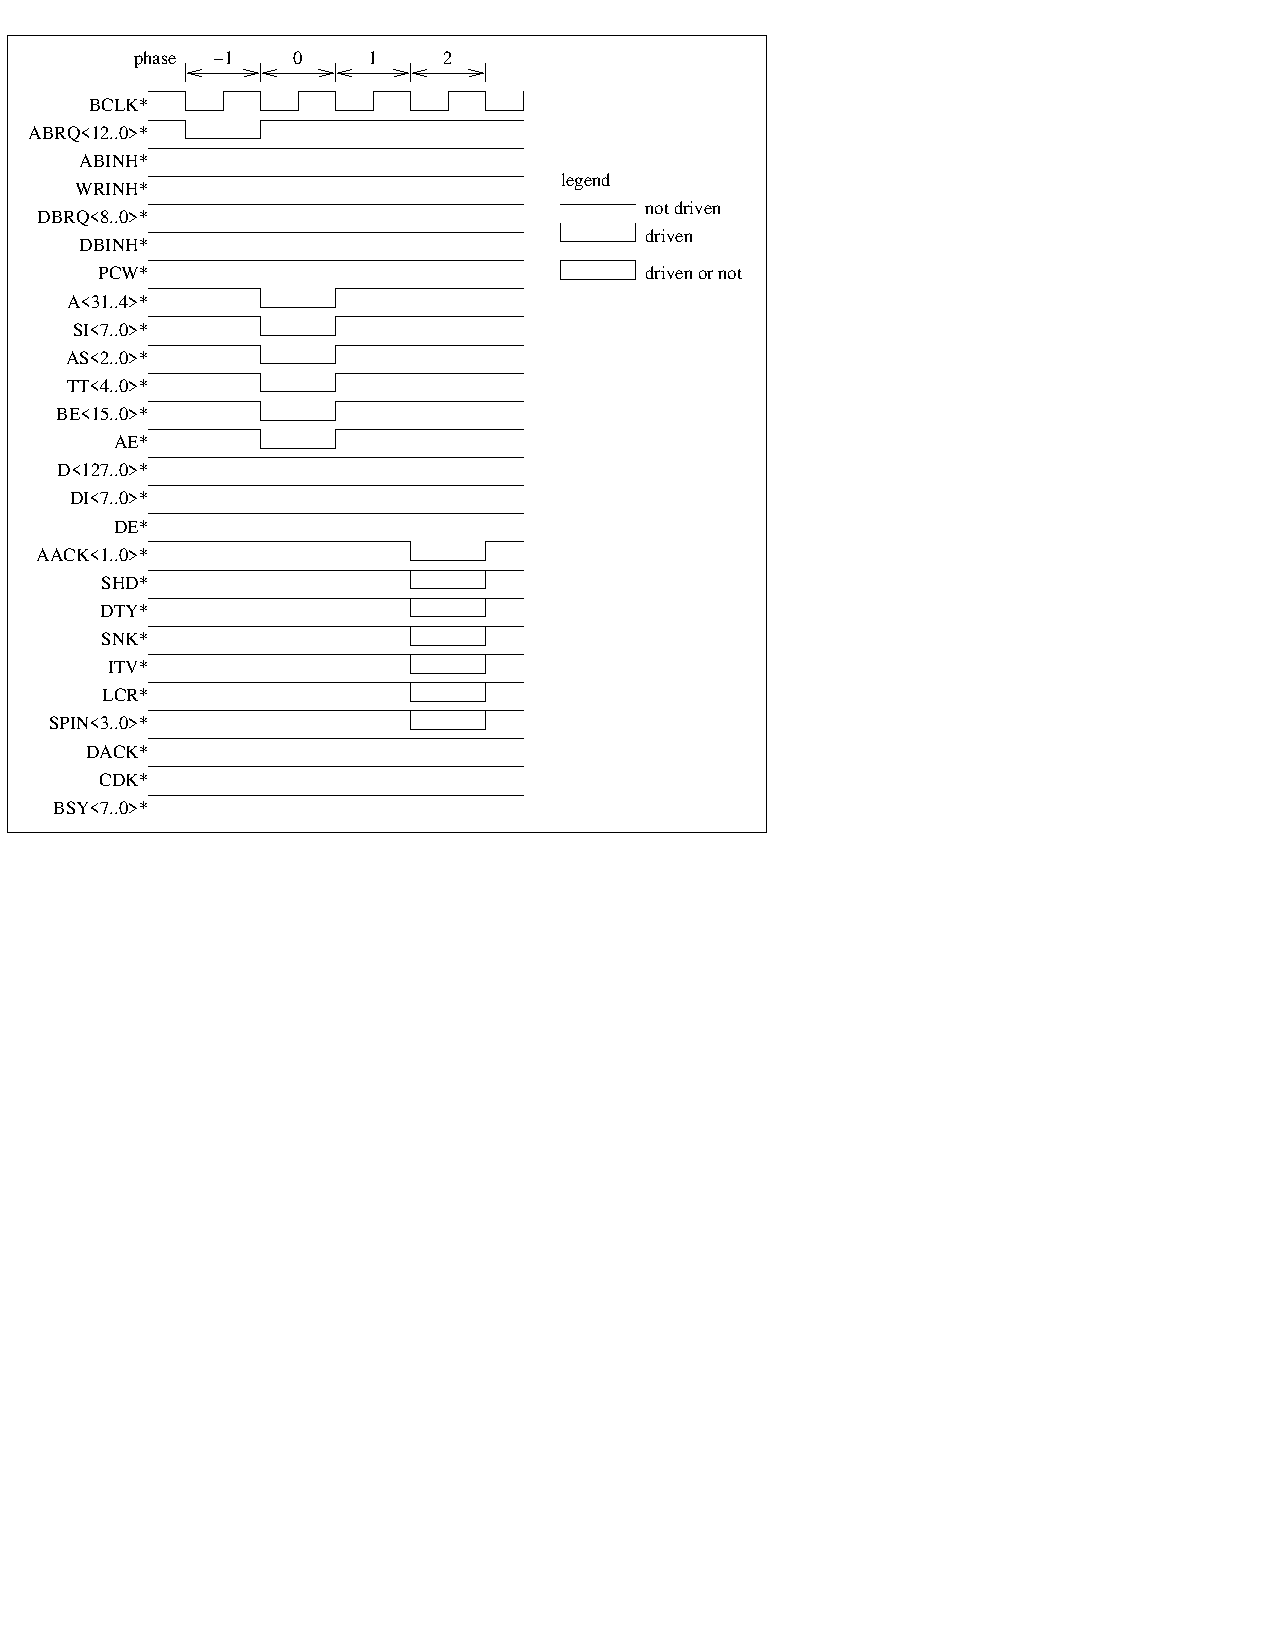
\includegraphics{ch3/FIG/single-add-basic.jpg}}
   \caption{어드레스 기본 사이클}\label{figure:single-add-basic}
\end{figure}
\begin{itemize}
	\item 어드레스 버스 중재 주기 - 단계 -1 (phase -1)\\
	어드레스 버스에 해당 어드레스를 구동하기에 앞서 수행하는 어드레스 버스 중재 주기.
	\item 어드레스 기본 주기 - 단계 0 (phase 0)\\
	중재 버스를 통하여 버스 사용허가를 받은 RQ가 한 버스 클럭 주기 동안 
	버스 상에 어드레스와 관련한 정보를 전송한다.
	32 비트의 어드레스, 어드레스 영역, 전송 형태, 바이트 마스크, RQ의 슬롯과
	채널 어드레스등과 각 신호의 패리티가 전송된다.
	이 주기 동안 사용되는 신호는 A$<$31..4$>$*, AP$<$3..0$>$*,
	AS$<$2..0$>$*, TT$<$4..0$>$*, STP*,
	BE$<$15..0$>$*, BEP$<$1..0$>$*,
	SI$<$7..0$>$*, SIP*, AE* 등이다.
	RP들은 이 단계의 끝 부분에서 어드레스 버스에 실린 신호를 모두 저장한다. \\
	캐쉬를 갖는 RQ 들도 이 단계의 끝 부분에서 어드레스 버스에 실린 신호를 모두 저장한다.
%
	\item 어드레스 기본 주기 - 단계 1 (phase 1)\\
	이 단계는 버스 상의 신호의 구동은 없다.
	단계 0에서 어드레스 버스를 구동했던 RQ는 다음 동작을 준비한다.
	단계 0에서 전송된 어드레스 등의 정보를 받은 RP들은 내부적으로  단계 2를 위한 동작이 수행된다.
	우선 RP는 각 정보의 패리티 에러 확인을 한다. 패리티 에러가 발견되지 않은 경우
	RP들은 저장한 어드레스를 번역하여 전송된 어드레스가 자신의 영역을 지정했는지를 확인한다.
	선택된 하나의 RP만 자신의 상태를 점검하여 단계 2에서 전송할 신호의 내용을 준비한다. \\
	캐쉬를 갖는 RQ들은 캐쉬 동일성 유지를 위한 동작을 내부적으로 수행한다.
%
	\item 어드레스 기본 주기 - 단계 2 (phase 2)\\
	단계 2에서는 어드레스에 의해 선정된 한 RP가 단계 0에서 전송된 정보들에
	대한 응답을 버스 상에 구동한다. 
	이때 사용되는 신호는 AACK$<$1..0$>$* 이고,
	단계 0에서 어드레스를 전송했던 RQ는 이 정보를 받아서 저장한다.
	이 단계 후의 RP와 RQ의 내부적인 동작은 기본 주기에서 규정하지 않는다.
	단계 1에서 패리티 에러가 검출된 경우 RP는 신호를 구동하지 않는다. \\
	캐쉬를 갖는 RQ들은 단계 0에서 저장한 어드레스에 대해 
	캐쉬 동일성 유지 동작을 수행함에 있어서 문제가 발생하면 SNK* 신호를 구동한다.
	또는 캐쉬 동일성 유지 동작에 필요한 SHD*, DTY*, ITV* 신호를
	구동한다.
\end{itemize}
%
\subsubsection{단일 전송 데이터 기본 사이클}
이미 수행된 어드레스 기본 사이클에서 데이터 요청이 발생한 경우 RP가 해당 어드레스의 데이터를
RQ로 전달할 때 사용하며 반드시 데이터 버스중재 과정을 거친 후에 수행된다.
데이터 버스 중재를 수행하여 데이터 버스 사용권을 획득한 바로 다음 버스 클럭 주기에
데이터 기본 사이클이 수행된다.
%\input{ch3/TBL/data-basic}
\begin{figure}[hp]
   \centerline{\includegraphics{ch3/FIG/single-data-basic.jpg}}
   \caption{데이터 기본 사이클}\label{figure:single-data-basic}
\end{figure}
\begin{itemize}
	\item 데이터 버스 중재 주기 - 단계 -1 (phase -1)\\
	데이터 버스에 해당 데이터를 구동하기에 앞서 수행하는 데이터 버스 중재 동작.
%
	\item 데이터 기본 주기 - 단계 0 (phase 0)\\
	데이터 중재 버스를 통하여 데이터 전송 버스의 사용 허가를 받은 RP가
	데이터 전송 버스의 신호들을 구동한다.
	구동되는 버스의 신호는 D$<$127..0$>$*, DP$<$15..0$>$*,
	DI$<$7..0$>$*, DIP*, DE* 등이다.
	데이터 신호는 어드레스 기본 주기에 의해 전송된 영역에 해당되는 데이터가 구동되고,
	종착점 신호(DI$<$7..0$>$*)는 전송하는 데이터를 요청했던
	RQ의 시발점 신호(SI$<$7..0$>$*)를 구동한다.
	어드레스 주기를 통하여 RP로 데이터 요청을 한 RQ들(2개 이상이 될 수 있음)은
	데이터 버스의 신호를 저장한다.
%
	\item 데이터 기본 주기 - 단계 1 (phase 1)\\
	단계 0에서 데이터 버스를 구동했던 RP는 다음 동작을 준비한다.
	단계 0에서 전송된 데이터 등의 정보를 받은 RQ는 내부적으로  단계 2를 위한 동작이 수행된다.
	우선 RQ들은 내부적으로 전송된 정보 들의 패리티 에러의 확인을 한다.
	에러가 발견되지 않으며, 종착점 신호를 자신의 슬롯 어드레스와 비교하여
	전송된 데이터가 자신이 요청한 것인지를 확인하게 된다.
	자신의 데이터가 아니면 데이터의 저장을 무효화한다.
%
	\item 데이터 기본 주기 - 단계 2 (phase 2)\\
	단계 1에서 전송된 정보 중에 패리티 에러가 발견되면 
	DACK*를 구동하지 않고, 패리티 에러가 없으면 DACK*를 구동하여 RP로부터 전송된
	데이터를 RQ가 잘 받았음을 알린다.
	특히 해당 데이터에서 패리티 에러가 발견된 경우 RQ는 그 데이터 전송을 있게 한 어드레스 전송까지 무효화하고,
	어드레스 기본 주기부터 재시도한다.
\end{itemize}
%
\subsubsection{블록 전송 데이터 기본 사이클}
이미 수행된 어드레스 기본 사이클에서 데이터 요청이 있은 경우 RP가 해당 어드레스의 데이터를
RQ로 전달할 때 사용하며 반드시 데이터 중재 과정을 거친 후에 수행된다.
데이터 중재를 수행하여 데이터 버스 사용권을 획득한 바로 다음 버스 클럭 주기에
데이터 기본 사이클이 수행된다.
%\input{ch3/TBL/data-basic}
\begin{figure}[hp]
   \centerline{\includegraphics{ch3/FIG/block-data-basic.jpg}}
   \caption{블록 전송 데이터 기본 사이클}\label{figure:block-data-basic}
\end{figure}
\begin{itemize}
	\item 블록 전송 데이터 버스 중재 주기 - 단계 -1 (phase -1)\\
	데이터 버스에 해당 데이터를 구동하기에 앞서 수행하는 데이터 버스 중재 동작. \\
	블록 전송 어드레스 데이터 기본 주기의 데이터 구동과 충돌을 방지하기 위해
	WRINH* 신호를 구동한다.
%
	\item 블록 전송 데이터 기본 주기 - 단계 0 (phase 0)\\
	데이터 중재 버스를 통하여 데이터 전송 버스의 사용 허가를 받은 RP가
	데이터 전송 버스의 신호들을 구동한다.
	구동되는 버스의 신호는 D$<$127..0$>$*, DP$<$15..0$>$*,
	DI$<$7..0$>$*, DIP*, DE* 등이다.
	데이터 신호는 어드레스 기본 주기에 의해 전송된 영역에 해당되는 데이터가 구동되고,
	종착점 신호(DI$<$7..0$>$*)는 전송하는 데이터를 요청했던
	RQ의 시발점 신호(SI$<$7..0$>$*)를 구동한다.
	어드레스 주기를 통하여 RP로 데이터 요청을 RQ는
	데이터 버스의 신호를 저장한다. \\
	블록 전송 어드레스 데이터 기본 주기의 데이터 구동에 충돌을 방지하기 위해
	WRINH* 신호를 구동한다.
	다른 블록 전송 데이터 기본 주기의 데이터 구동과 충돌을 방지하기 위해
	DBINH* 신호를 구동한다.
%
	\item 블록 전송 데이터 기본 주기 - 단계 1 (phase 1)\\
	데이터 전송 버스의 신호들을 구동한다.
	구동되는 버스의 신호는 D$<$127..0$>$*, DP$<$15..0$>$*,
	DI$<$7..0$>$*, DIP*, DE* 등이다.
	데이터 신호는 어드레스 기본 주기에 의해 전송된 영역에 해당되는 데이터가 구동되고,
	종착점 신호(DI$<$7..0$>$*)는 전송하는 데이터를 요청했던
	RQ의 시발점 신호(SI$<$7..0$>$*)를 구동한다.
	어드레스 주기를 통하여 RP로 데이터를 요청한 RQ는
	데이터 버스의 신호를 저장한다. \\
	단계 0에서 데이터 버스를 구동했던 RP는 다음 동작을 준비한다.
	단계 0에서 전송된 데이터등의 정보를 받은 RP들은 내부적으로  단계 2를 위한 동작을 수행한다.
	우선 RQ들은 내부적으로 전송된 정보들의 패리티 에러의 유무를 확인한다.
	에러가 발견되지 않으며, 종착점 신호를 자신의 슬롯 어드레스와 비교하여
	전송된 데이터가 자신이 요청한 것인지를 확인하게 된다.
	자신의 데이터가 아니면 데이터의 저장을 무효화한다. \\
	블록 전송 어드레스 데이터 기본 주기의 데이터 구동에 충돌을 방지하기 위해
	WRINH* 신호를 구동한다.
	다른 블록 전송 데이터 기본 주기의 데이터 구동과 충돌을 방지하기 위해
	DBINH* 신호를 구동한다.
%
	\item 블록 전송 데이터 기본 주기 - 단계 2 (phase 2)\\
	데이터 전송 버스의 신호들을 구동한다.
	구동되는 버스의 신호는 D$<$127..0$>$*, DP$<$15..0$>$*,
	DI$<$7..0$>$*, DIP*, DE* 등이다.
	데이터 신호는 어드레스 기본 주기에 의해 전송된 영역에 해당되는 데이터가 구동되고,
	종착점 신호(DI$<$7..0$>$*)는 전송하는 데이터를 요청했던
	RQ의 시발점 신호(SI$<$7..0$>$*)를 구동한다.
	어드레스 주기를 통하여 RP로 데이터를 요청한 RQ는
	데이터 버스의 신호를 저장한다. \\
	단계 0에서 전송된 정보 중에 패리티 에러가 발견되면 
	DACK*를 구동하지 않고, 패리티 에러가 없으면 DACK*를 구동하여 RP로부터 전송된
	데이터를 RQ가 잘 받았음을 알린다.
	특히 해당 데이터에서 패리티 에러가 발견된 경우 RQ는 어드레스 기본 주기부터 재시도 한다. \\
	다른 블록 전송 데이터 기본 주기의 데이터 구동과 충돌을 방지하기 위해
	DBINH* 신호를 구동한다.
%
	\item 블록 전송 데이터 기본 주기 - 단계 3 (phase 3)\\
	데이터 전송 버스의 신호들을 구동한다.
	구동되는 버스의 신호는 D$<$127..0$>$*, DP$<$15..0$>$*,
	DI$<$7..0$>$*, DIP*, DE* 등이다.
	데이터 신호는 어드레스 기본 주기에 의해 전송된 영역에 해당되는 데이터가 구동되고,
	종착점 신호(DI$<$7..0$>$*)는 전송하는 데이터를 요청했던
	RQ의 시발점 신호(SI$<$7..0$>$*)를 구동한다.
	어드레스 주기를 통하여 RP로 데이터를 요청한 RQ는
	데이터 버스의 신호를 저장한다. \\
	단계 1에서 전송된 정보 중에 패리티 에러가 발견되면 
	DACK*를 구동하지 않고, 패리티 에러가 없으면 DACK*를 구동하여 RP로부터 전송된
	데이터를 RQ가 잘 받았음을 알린다.
	특히 해당 데이터에서 패리티 에러가 발견된 경우 RQ는 그 데이터 전송을 있게 한 어드레스 전송까지 무효화하고,
	어드레스 기본 주기부터 재시도한다.
	\item 블록 전송 데이터 기본 주기 - 단계 4 (phase 4)\\
	단계 2에서 전송된 정보 중에 패리티 에러가 발견되면 
	DACK*를 구동하지 않고, 패리티 에러가 없으면 DACK*를 구동하여 RP로부터 전송된
	데이터를 RQ가 잘 받았음을 알린다.
	특히 해당 데이터에서 패리티 에러가 발견된 경우 RQ는
	어드레스 기본 주기부터 재시도한다.
	\item 블록 전송 데이터 기본 주기 - 단계 5 (phase 5)\\
	단계 3에서 전송된 정보 중에 패리티 에러가 발견되면 
	DACK*를 구동하지 않고, 패리티 에러가 없으면 DACK*를 구동하여 RP로부터 전송된
	데이터를 RQ가 잘 받았음을 알린다.
	특히 해당 데이터에서 패리티 에러가 발견된 경우 RQ는
	어드레스 기본 주기부터 재시도한다.
\end{itemize}
%
\subsubsection{단일 전송 어드레스-데이터 기본 사이클}
어드레스 정보(어드레스와 이에 관련된 정보들)와 데이터 정보(데이터와 이에 관견된 정보들)를
동시에 전달할 때 사용하는
기본 사이클이며 반드시 어드레스 중재 과정을 거친 후에 수행되어야 한다.
이 기본 사이클은 4개의 단계로 구성되며 각 단계는 연속적이다.
어드레스 중재를 수행하여 어드레스 버스 사용권을 획득한 바로 다음 버스 클럭 주기에 어드레스-데이터 기본 사이클의
단계 0(phase 0)가 시작된다. RQ는 단계 0에서 어드레스 정보를
어드레스 버스에 구동한다. 단계 1에서는 각 RP들이 단계 0에 전달된 어드레스 정보를 번역하여
필요한 동작을 준비한다. 이때 RQ는 데이터 정보를 데이터 버스에 구동한다.
단계 2에서는 단계 1에서 결정된 RP가 전달받은 어드레스 정보에 대한 응답(어드레스 응답)을 구동하며,
동시에 단계 1에서 전달된 데이터를 점검한다.
단계 3에서는 RP가 단계 1에서 전달받은 데이터에 대한 데이터 응답을 구동한다.
RQ는 단계 2에 전달받은 어드레스 응답과 단계 3에 전달받은 데이터 응답에 의해
수행한 어드레스-데이터 기본 사이클의 완성 여부를 판단한다.
%\input{ch3/TBL/add-data-basic}
\begin{figure}[hp]
   \centerline{\includegraphics{ch3/FIG/single-add-data-basic.jpg}}
   \caption{어드레스 데이터 기본 사이클}\label{figure:single-add-data-basic}
\end{figure}
\begin{itemize}
	\item 단일 전송 어드레스 버스 중재 주기 - 단계 -1 (phase -1)\\
	어드레스 버스에 해당 어드레스를 구동하기에 앞서 수행하는 어드레스 버스 중재 동작.
	\item 단일 전송 어드레스 데이터 기본 주기 - 단계 0 (phase 0)\\
	중재 버스를 통하여 버스 사용허가를 받은 RQ가 한 버스 클럭 주기 동안 
	버스 상에 어드레스와 관련한 정보를 전송한다.
	32 비트의 어드레스, 어드레스 영역, 전송 형태, 바이트 마스크, RQ의 슬롯과
 	채널 어드레스등과 각 신호의 패리티가 전송된다.
	이 주기 동안 사용되는 신호는 A$<$31..4$>$*, AP$<$3..0$>$*,
	AS$<$2..0$>$*, TT$<$4..0$>$*, STP*,
	BE$<$15..0$>$*, BEP$<$1..0$>$*,
	SI$<$7..0$>$*, SIP*, AE* 등이다.
	RP들은 이 단계의 끝 부분에서 어드레스 버스에 실린 신호를 모두 저장한다. \\
	캐쉬를 갖는 RQ들도 이 단계의 끝 부분에서 어드레스 버스에 실린 신호를 모두 저장한다. \\
	데이터 기본주기와의 데이터 충돌을 방지하기 위해 DBINH* 신호를 구동한다.
%
	\item 단일 전송 어드레스 데이터 기본 주기 - 단계 1 (phase 1)\\
	단계 0를 구동한 RQ가 계속해서 데이터 버스를 구동한다.
	이 단계에서 구동되는 신호선은 D$<$127..0$>$*,
	DP$<$15..0$>$*, DI$<$7..0$>$*, DIP*, DE*등이다.
	데이터 기본 주기와는 달리 별도의 데이터 중재 과정이 없다.\\
	RP들은 단계 0에서 저장한 어드레스 버스의 정보들의 에러 확인과 번역을 수행한다.
	또한 단계 1의 부분에서는 RQ로부터 오는 데이터를 저장한다. \\
	캐쉬를 갖는 RQ들은 캐쉬 동일성 유지를 위한 동작을 내부적으로 수행한다.
%
	\item 단일 전송 어드레스 데이터 기본 주기 - 단계 2 (phase 2)\\
	단계 2에서는 어드레스에 의해 선정된 한 RP가 단계 0에서 전송된 정보들에
	대한 응답을 버스 상에 구동하고 단계 1에서 받은 데이터의 패리티 에러를 확인한다.
	이때 사용되는 신호는 AACK$<$1..0$>$* 이고,
	만약 단계 0에서 전송된 정보에 에러가 검출될 경우 신호 구동과 데이터 패리티 확인을
	수행하지 않는다. \\
	캐쉬를 갖는 RQ 들이 단계 0에서 저장한 어드레스에 대한 
	캐쉬 동일성 유지 동작을 수행함에 있어서 문제가 발생하면 SNK* 신호를 구동한다.
	단계 0를 수행했던 RQ는 어드레스 상태 신호를 저장한다. \\
%
	\item 단일 전송 어드레스 데이터 기본 주기 - 단계 3 (phase 3)\\
	단계 1에서 전송된 데이터를 받은 RP가 RQ로 응답하는 단계이다.
	데이터의 에러 유무를 보고한다. 이때 사용하는 신호선은 DACK*이다.
	단계 2의 응답에서 어드레스를 정상적으로 접수하지 못했다는 반응이 있었을 경우
	이 단계의 응답은 의미가 없다. \\
	RQ는 데이터 응답을 저장한다. \\
\end{itemize}
%
\subsubsection{블록 전송 어드레스-데이터 기본 사이클}
어드레스 정보(어드레스와 이에 관련된 정보들)와 데이터 정보(데이터와 이에 관견된 정보들)를
동시에 전달할 때 사용하는
기본 사이클이며 반드시 어드레스 중재 과정을 거친 후에 수행되어야 한다.
이 기본 사이클은 4개의 단계로 구성되며 각 단계는 연속적이다.
어드레스 중재를 수행하여 어드레스 버스 사용권을 획득한 바로 다음 버스 클럭 주기에 어드레스-데이터 기본 사이클의
단계 0(phase 0)가 시작된다. RQ는 단계 0에서는 어드레스 정보를
어드레스 버스에 구동한다. 단계 1에서는 각 RP들이 단계 0에 전달된 어드레스 정보를 번역하여
필요한 동작을 준비한다. 이때 RQ는 데이터 정보를 데이터 버스에 구동한다.
단계 2에서는 단계 0에서 결정된 RP가 전달받은 어드레스 정보에 대한 응답(어드레스 응답)을 구동하며,
동시에 단계 0에서 전달된 데이터를 점검한다.
단계 3에서는 RP가 단계 1에서 전달받은 데이터에 대한 데이터 응답을 구동한다.
RQ는 단계 2에 전달받은 어드레스 응답과 단계 3에 전달받은 데이터 응답에 의해
수행한 어드레스-데이터 기본 사이클의 완성 여부를 판단한다.
%\input{ch3/TBL/add-data-basic}
\begin{figure}[hp]
   \centerline{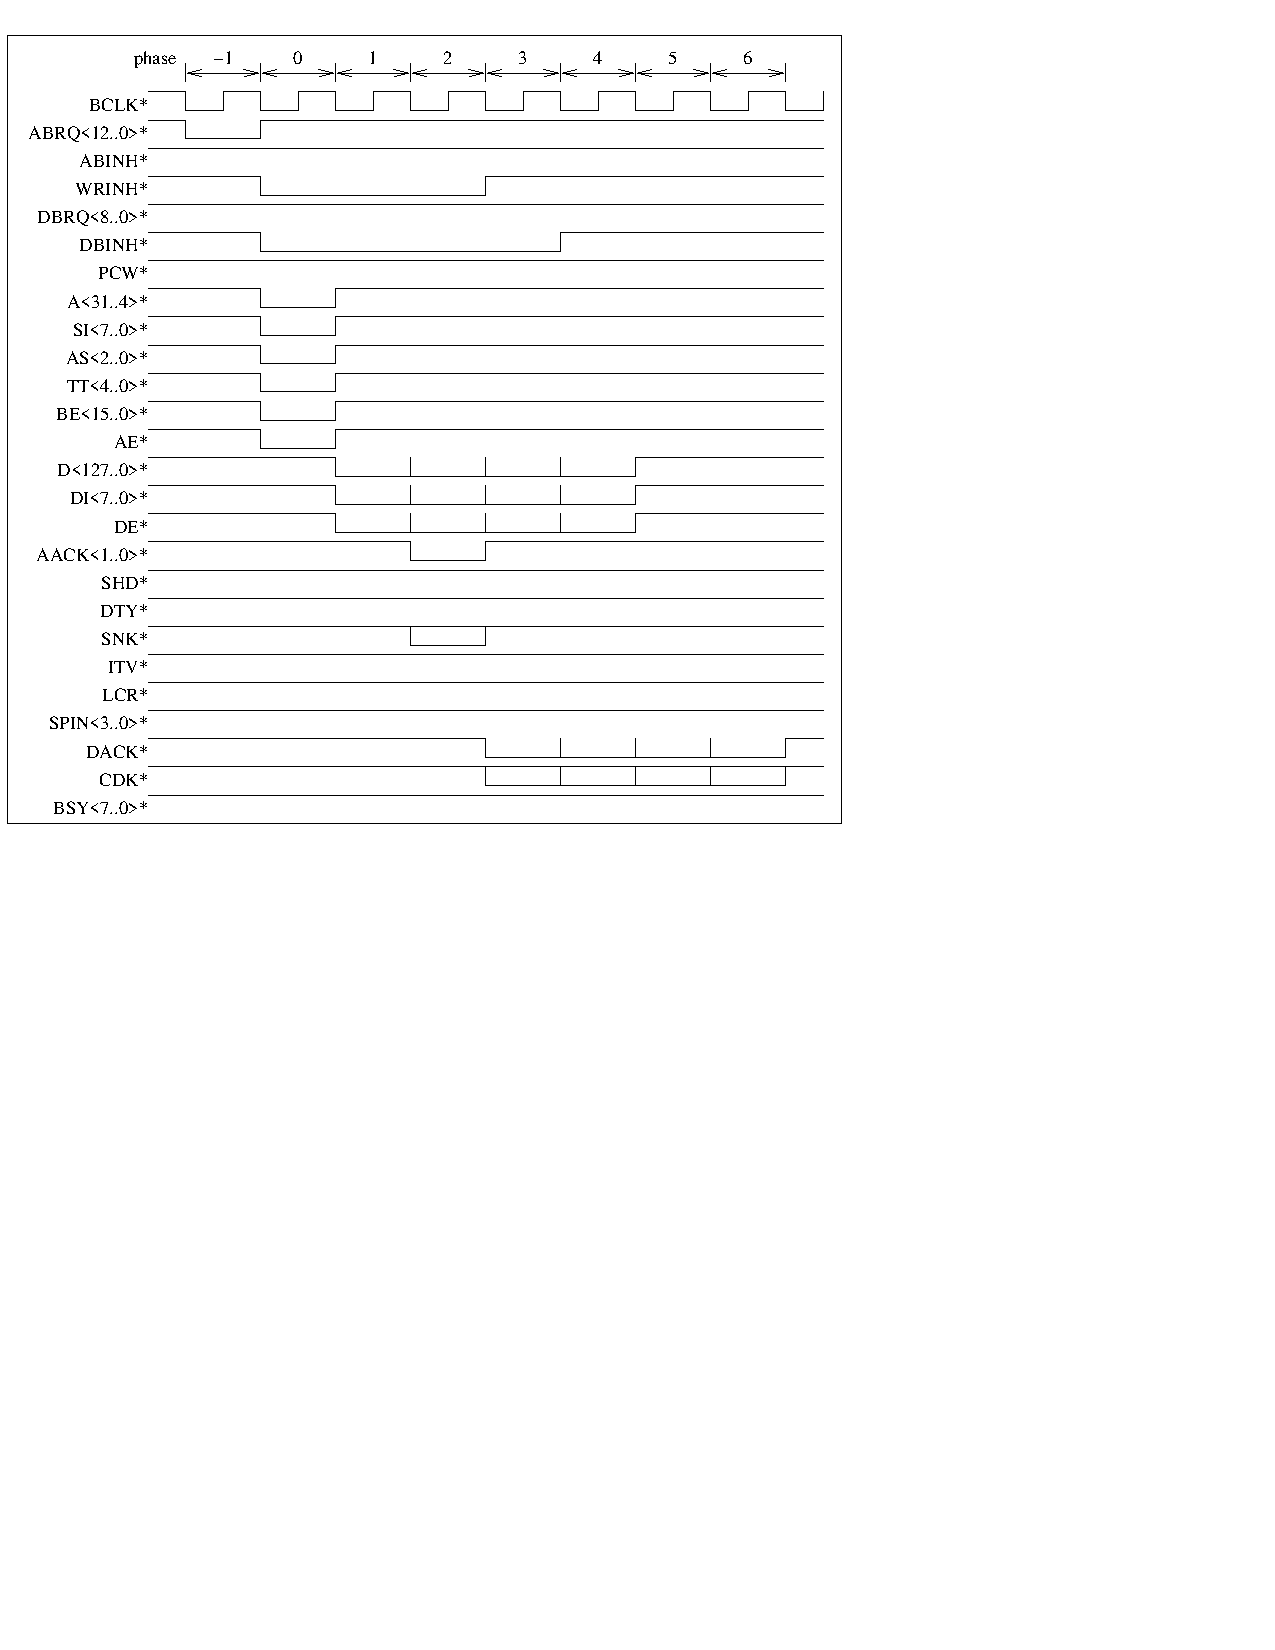
\includegraphics{ch3/FIG/block-add-data-basic.jpg}}
   \caption{블록 전송 어드레스 데이터 기본 사이클}\label{figure:block-add-data-basic}
\end{figure}
\begin{itemize}
	\item 블록 전송 어드레스 버스 중재 주기 - 단계 -1 (phase -1)\\
	어드레스 버스에 해당 어드레스를 구동하기에 앞서 수행하는 어드레스 버스 중재 동작.
	\item 블록 전송 어드레스 데이터 기본 주기 - 단계 0 (phase 0)\\
	중재 버스를 통하여 버스 사용허가를 받은 RQ가 한 버스 클럭 주기 동안 
	버스 상에 어드레스와 관련한 정보를 전송한다.
	32 비트의 어드레스, 어드레스 영역, 전송 형태, 바이트 마스크, RQ의 슬롯과
	채널 어드레스등과 각 신호의 패리티가 전송된다.
	이 주기 동안 사용되는 신호는 A$<$31..4$>$*, AP$<$3..0$>$*,
	AS$<$2..0$>$*, TT$<$4..0$>$*, STP*,
	BE$<$15..0$>$*, BEP$<$1..0$>$*,
	SI$<$7..0$>$*, SIP*, AE*등이다.
	RP들은 이 단계의 끝 부분에서 어드레스 버스에 실린 신호를 모두 저장한다. \\
	캐쉬를 갖는 RQ들도 이 단계의 끝 부분에서 어드레스 버스에 실린 신호를 모두 저장한다. \\
	다른 블록 전송 쓰기와의 데이터 충돌을 방지하기 위해 WRINH* 신호를 구동한다.
	다른 전송의 데이터와 충돌을 방지하기 위해 DBINH* 신호를 구동한다.
%
	\item 블록 전송 어드레스 데이터 기본 주기 - 단계 1 (phase 1)\\
	단계 0를 구동한 RQ가 계속해서 데이터 버스를 구동한다.
	이 단계에서 구동되는 신호선은 D$<$127..0$>$*,
	DP$<$15..0$>$*, DI$<$7..0$>$*, DIP*, DE*등이다.
	데이터 기본 주기와는 달리 별도의 데이터 중재 과정이 없다. \\
%	따라서 데이터 주기를 수행하고자 하는 RP와 충돌이 발생하지 않토록 데이터 중재기들은
%	어드레스 데이터 주기의 단계 1에서는 중재를 수행하지 않는다. \\
	RP들은 단계 0에서 저장한 어드레스 버스의 정보들의 에러 확인과 번역을 수행한다.
	또한 단계 1의 부분에서는 RQ로부터 오는 데이터를 저장한다. \\
	캐쉬를 갖는 RQ들은 캐쉬 동일성 유지를 위한 동작을 내부적으로 수행한다. \\
	다른 블록 전송 쓰기와의 데이터 충돌을 방지하기 위해 WRINH* 신호를 구동한다.
	다른 전송의 데이터와 충돌을 방지하기 위해 DBINH* 신호를 구동한다.
%
	\item 블록 전송 어드레스 데이터 기본 주기 - 단계 2 (phase 2)\\
	단계 2에서는 어드레스에 의해 선정된 한 RP가 단계 0에서 전송된 정보들에
	대한 응답을 버스 상에 구동하고 단계 1에서 받은 데이터의 패리티 에러를 확인한다.
	이때 사용되는 신호는 AACK$<$1..0$>$* 이고,
	만약 단계 0에서 전송된 정보에 에러가 검출될 경우 신호 구동과 데이터 패리티 확인을
	수행하지 않는다. \\
	단계 0를 구동한 RQ가 계속해서 데이터 버스를 구동한다.
	이 단계에서 구동되는 신호선은 D$<$127..0$>$*,
	DP$<$15..0$>$*, DI$<$7..0$>$*, DIP*, DE*등이다.
	데이터 기본 주기와는 달리 별도의 데이터 중재 과정이 없다. \\
	캐쉬를 갖는 RQ들이 단계 0에서 저장한 어드레스에 대한 
	캐쉬 동일성 유지 동작을 수행함에 있어서 문제가 발생하면 SNK* 신호를 구동한다.
	단계 0를 수행했던 RQ는 어드레스 상태 신호를 저장한다. \\
	다른 블록 전송 어드레스 데이터 기본주기와의 데이터 충돌을 방지하기 위해 WRINH* 신호를 구동한다.
	다른 전송의 데이터와 충돌을 방지하기 위해 DBINH* 신호를 구동한다.
%
	\item 블록 전송 어드레스 데이터 기본 주기 - 단계 3 (phase 3)\\
	단계 1에서 전송된 데이터를 받은 RP가 RQ로 응답하는 단계이다.
	데이터의 에러 유무를 보고한다. 이때 사용하는 신호선은 DACK*이다.
	그러나 현재 진행 중인 전송이 ITW인 경우 DACK*는 의미가 없고 대신 CDK*가 사용된다.
	단계 2의 응답에서 어드레스를 정상적으로 접수하지 못했다는 반응이 있었을 경우
	이 단계의 응답은 의미가 없다. \\
	단계 0를 구동한 RQ가 계속해서 데이터 버스를 구동한다.
	이 단계에서 구동되는 신호선은 D$<$127..0$>$*,
	DP$<$15..0$>$*, DI$<$7..0$>$*, DIP*, DE*등이다.
	데이터 기본 주기와는 달리 별도의 데이터 중재 과정이 없다. \\
	단계 0에 구동된 어드레스에 의해 선택된 RP는
	단계 1에 구동된 데이터에 대한 데이터 응답 DACK*을 구동하고,
	RQ는 해당 데이터 응답을 저장한다.
	그러나 현재 진행중인 전송이 ITW인 경우 DACK*는 의미가 없고 대신 CDK*가 사용된다.\\
	다른 전송의 데이터와 충돌을 방지하기 위해 DBINH* 신호를 구동한다.
%
	\item 블록 전송 어드레스 데이터 기본 주기 - 단계 4 (phase 4)\\
	단계 2에서 전송된 데이터를 받은 RP가 RQ로 응답하는 단계이다.
	데이터의 에러 유무를 보고한다. 이때 사용하는 신호선은 DACK* 이다.
	그러나 현재 진행 중인 전송이 ITW인 경우 DACK*는 의미가 없고 대신 CDK*가 사용된다.
	단계 2의 응답에서 어드레스를 정상적으로 접수하지 못했다는 반응이 있었을 경우
	이 단계의 응답은 의미가 없다. \\
	단계 0를 구동한 RQ가 계속해서 데이터 버스를 구동한다.
	이 단계에서 구동되는 신호선은 D$<$127..0$>$*,
	DP$<$15..0$>$*, DI$<$7..0$>$*, DIP*, DE*등이다.
	데이터 기본 주기와는 달리 별도의 데이터 중재 과정이 없다. \\
	단계 0에 구동된 어드레스에 의해 선택된 RP는
	단계 2에 구동된 데이터에 대한 데이터 응답을 구동하고, RQ는 해당 데이터 응답을 저장한다. \\
%
	\item 블록 전송 어드레스 데이터 기본 주기 - 단계 5 (phase 5)\\
	단계 3에서 전송된 데이터를 받은 RP가 RQ로 응답하는 단계이다.
	데이터의 에러 유무를 보고한다. 이때 사용하는 신호선은 DACK*이다.
	그러나 현재 진행중인 전송이 ITW인 경우 DACK*는 의미가 없고 대신 CDK*가 사용된다.
	단계 2의 응답에서 어드레스를 정상적으로 접수하지 못했다는 반응이 있었을 경우
	이 단계의 응답은 의미가 없다. \\
	단계 0에 구동된 어드레스에 의해 선택된 RP는
	단계 3에 구동된 데이터에 대한 데이터 응답을 구동하고, RQ는 해당 데이터 응답을 저장한다. \\
%
	\item 블록 전송 어드레스 데이터 기본 주기 - 단계 6 (phase 6)\\
	단계 4에서 전송된 데이터를 받은 RP가 RQ로 응답하는 단계이다.
	데이터의 에러 유무를 보고한다. 이때 사용하는 신호선은 DACK* 이다.
	그러나 현재 진행 중인 전송이 ITW인 경우 DACK*는 의미가 없고 대신 CDK*가 사용된다.
	단계 2의 응답에서 어드레스를 정상적으로 접수하지 못했다는 반응이 있었을 경우
	이 단계의 응답은 의미가 없다. \\
	단계 0에 구동된 어드레스에 의해 선택된 RP는
	단계 4에 구동된 데이터에 대한 데이터 응답을 구동하고, RQ는 해당 데이터 응답을 저장한다. \\
%
\end{itemize}
%
%
\subsection{전송의 구분}
정의된 전송의 종류는 NRD, NWR, NCR, NCW, IVD,
ILR, ILW, BRD, BWR, CRD, EXR, WRB, ITW로
13 가지이지만 실제 데이터가 이동되는 것은 IVD를 제외한 12 가지 전송형태이다.
그리고 데이터 이동이 수반되는 전송형태는 데이터의 실제 이동 방향에 따라
읽기 전송 모임(read transfer class)과 쓰기 전송 모임(write transfer class)으로 구분할 수 있다.
읽기 전송 모임은 데이터가 RP로부터 RQ로 이동하는 경우로써 NRD, NCR, CRD, EXR, BRD,
그리고 ILR가 여기에 속한다.
쓰기 전송 모임은 데이터가 RQ에서 RP로 이동하는 경우로써 NWR, NCW, WRB, BWR, 그리고 ILW가 여기에 속한다.
특히 ITW의 경우는 쓰기 전송과 비슷하지만 데이타는 RQ에서 RQ로 이동한다.
그리고 이동하는 데이터의 크기에 따라 단일 전송과 블록 전송으로 구분되며,
단일 전송의 경우 16바이트 이내의 연속된 데이터 전송에 사용되고,
블록 전송의 경우 64바이트 데이터 전송에 사용된다.
단일 전송에는 NRD, NWR, NCR, NCW, ILR, ILW가 있고,
블록 전송에는 BRD, BWR, CRD, EXR, WRB, ITW가 있다.
%
\subsubsection{단일 읽기 전송 모임}
단일 전송 읽기 전송은 단일 전송 어드레스 기본 사이클과 단일 전송 데이터 기본 사이클로 구성된다.
데이터가 필요한 RQ가 어드레스 기본 사이클을 수행하고, 어드레스 기본 사이클에 구동된 어드레스에 의해
선택된 RP는 단일 전송 데이터 기본 사이클을 수행하여 요청된 데이터를 전송하게 된다.
$<$그림~\ref{figure:single-read}$>$는 읽기 전송 모임의 진행 순서를 나타낸다.
%\input{ch3/TBL/read-class}
\begin{figure}[hp]
   \centerline{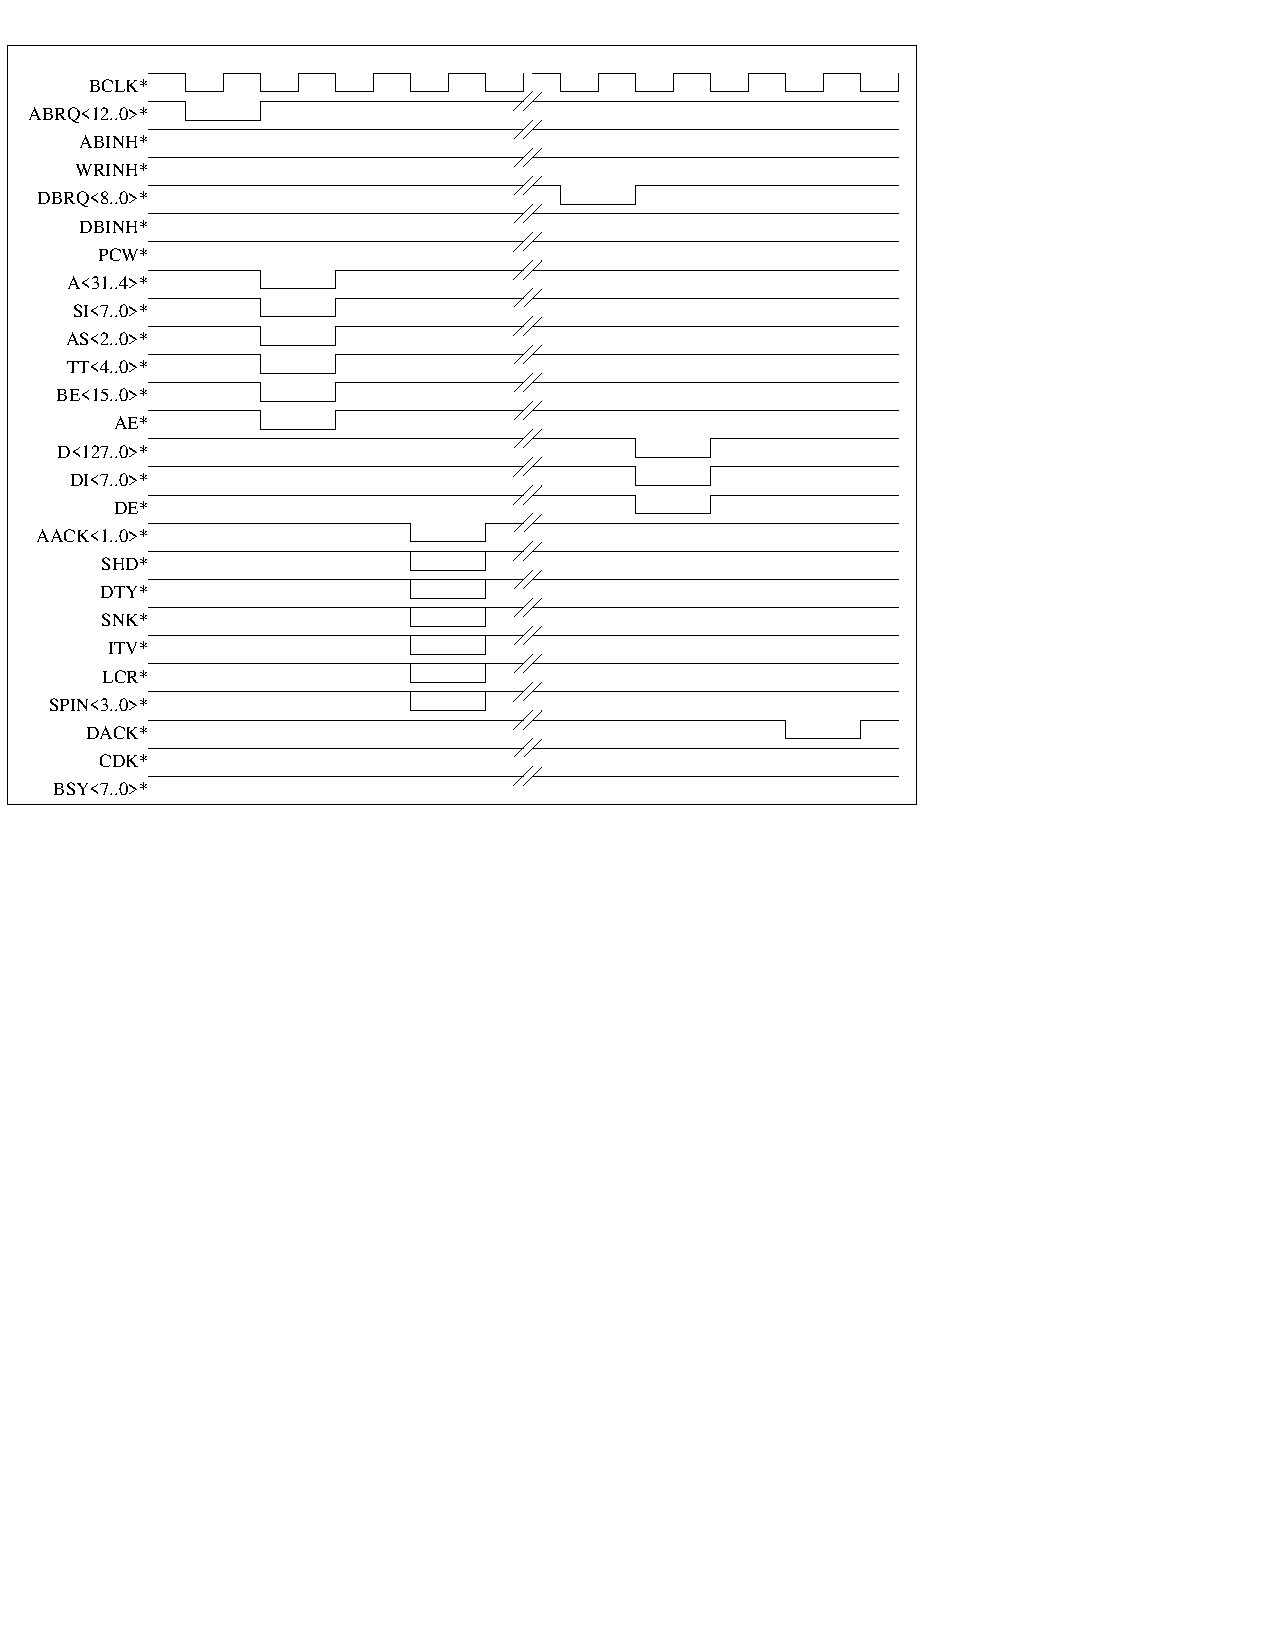
\includegraphics{ch3/FIG/single-read.jpg}}
   \caption{단일 읽기 전송}\label{figure:single-read}
\end{figure}
%
\subsubsection{단일 쓰기 전송 모임}
단일 전송 쓰기 전송은 단일 전송 어드레스 데이터 기본 사이클로 구성된다.
특정 RQ가 특정 RP로 데이터를 공급하는 전송이다.
$<$그림~\ref{figure:single-write}$>$는 쓰기 전송 모임의 진행 순서를 나타낸다.
%input{ch3/TBL/write-class}
\begin{figure}[hp]
   \centerline{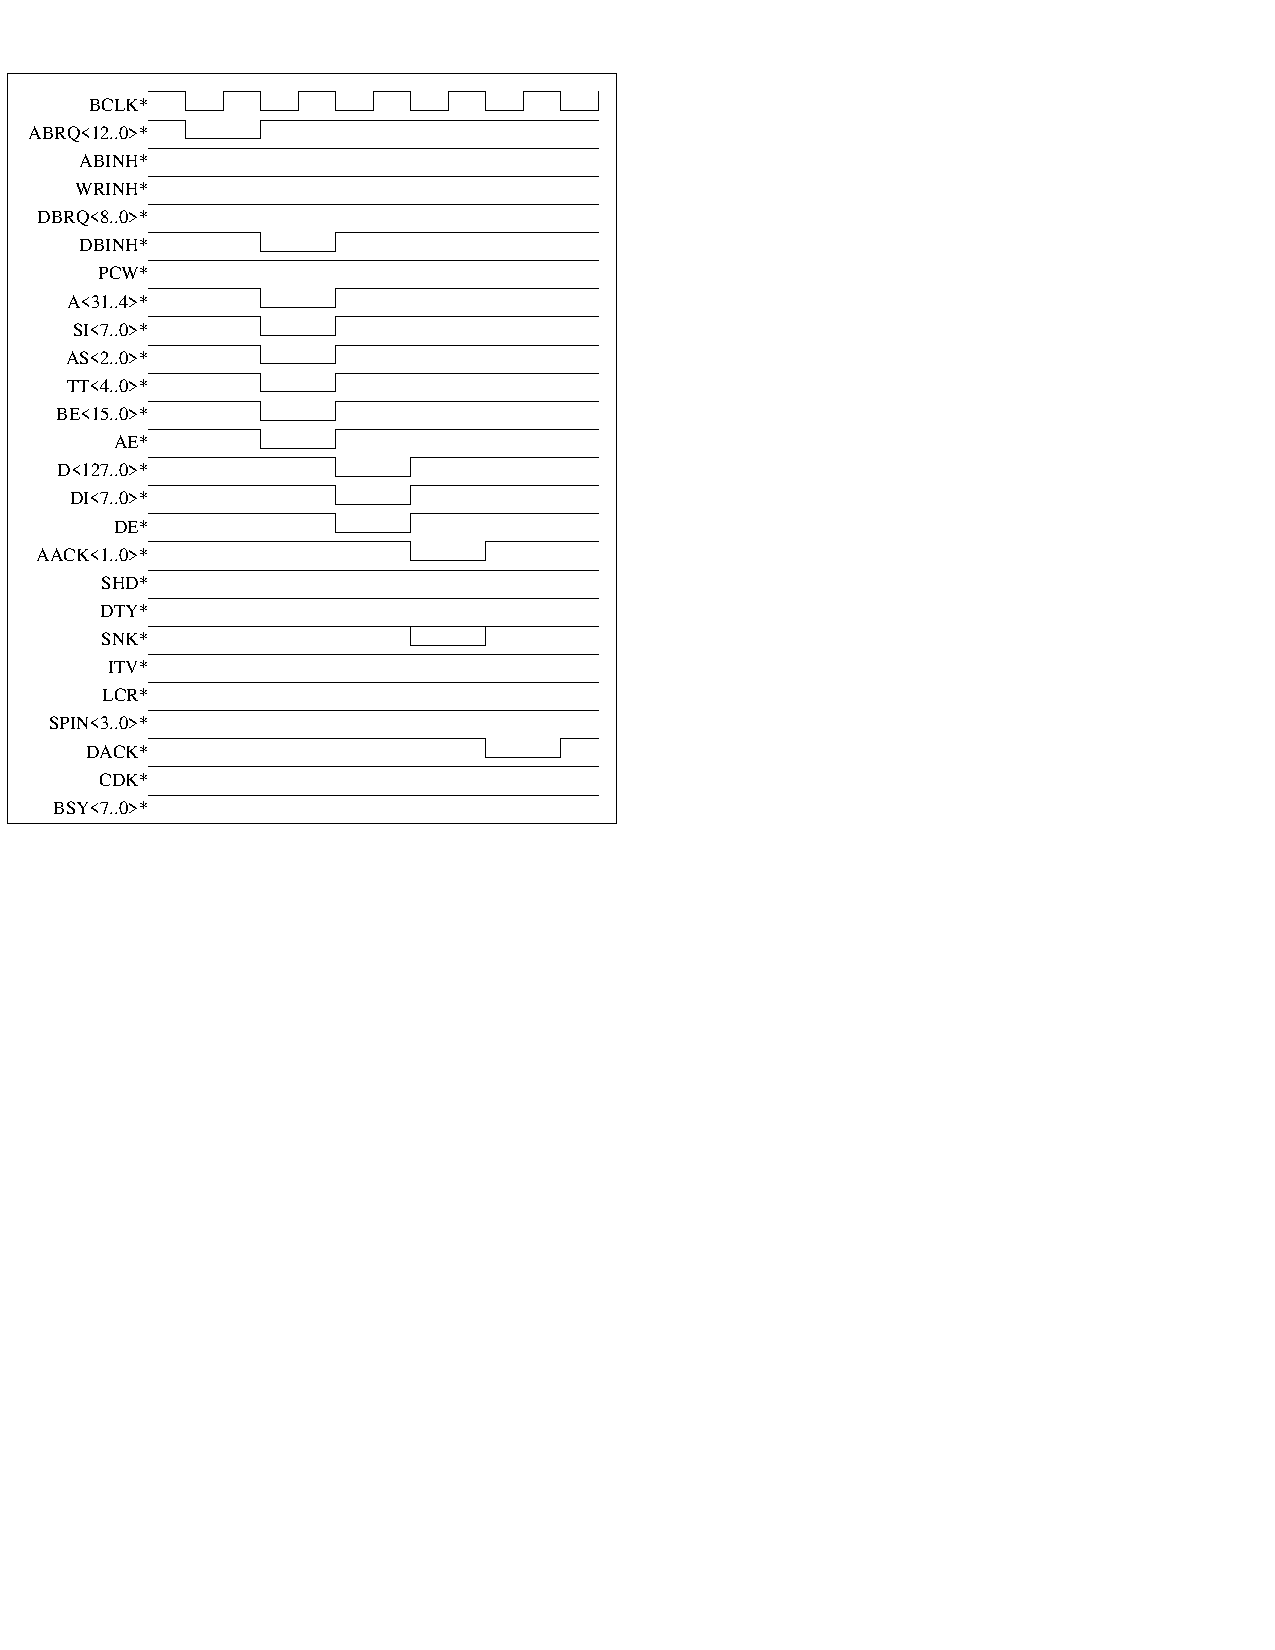
\includegraphics{ch3/FIG/single-write.jpg}}
   \caption{단일 쓰기 전송}\label{figure:single-write}
\end{figure}
%
\subsubsection{블록 읽기 전송 모임}
블록 전송 읽기 전송은 블록 전송 어드레스 기본 사이클과 블록 전송 데이터 기본 사이클로 구성된다.
데이터가 필요한 RQ가 어드레스 기본 사이클을 수행하고, 어드레스 기본 사이클에 구동된 어드레스에 의해
선택된 RP는 블록 전송 데이터 기본 사이클을 수행하여 요청된 데이터를 전송하게 된다.
\begin{figure}[hp]
   \centerline{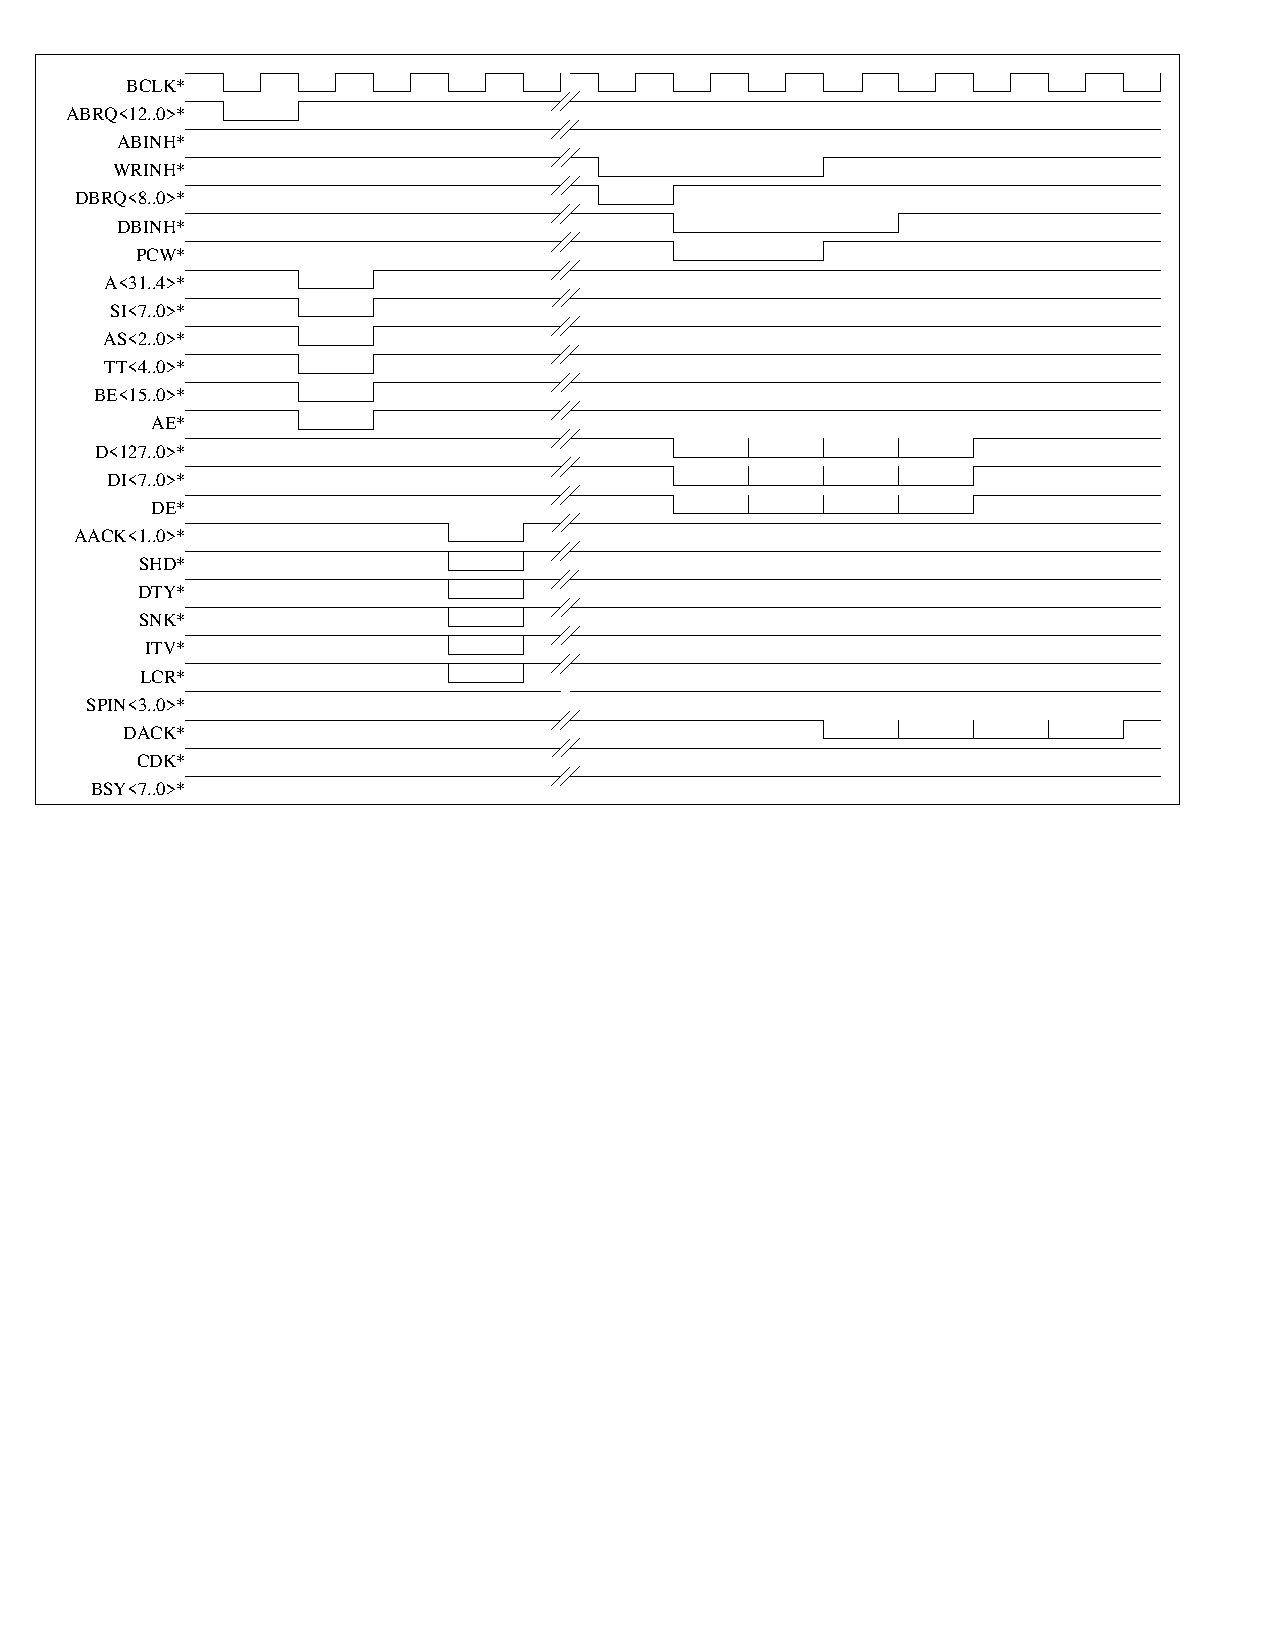
\includegraphics[angle=90]{ch3/FIG/block-read.jpg}}
   \caption{블록 읽기 전송}\label{figure:block-read}
\end{figure}
%
\subsubsection{블록 쓰기 전송 모임}
블록 전송 쓰기 전송은 블록 전송 어드레스 데이터 기본 사이클로 구성된다.
특정 RQ에서 특정 RP로, 혹은 특정 RQ에서 다른 특정 RQ로 데이터를 공급하는 전송이다.
\begin{figure}[hp]
   \centerline{\includegraphics{ch3/FIG/block-write.jpg}}
   \caption{블록 쓰기 전송}\label{figure:block-write}
\end{figure}
%%%%%
%\end{document}
%%%%%

\newpage
%%%%%
%%Title: HiPi+Bus V0.2 Chapter 3 Section 1
%%Creator: Ando Ki
%%CreationDate: April 1992
%%FileName: sec4
%%RelatedFile: ch3
%%%%%
%\documentstyle[doublespace,a4wide]{hbook}
%\setstretch{1.2}
%\pagestyle{headings}
%\begin{document}
%\pagenumbering{arabic}
%\setcounter{chapter}{1}
%
\section{예외 처리 (Exception Handling)}
예외 처리란 지금까지 정의한 동작 규정 중에서 정상적으로 동작이 완료되지 않고
에러가 발생했거나 특별한 상황이 발생했을 때, 이의 처리를 말한다. 

\subsection{패리티 에러 (Parity Error)}
패리티는 데이터 전송 버스의 신호 전송에 있어서 에러의 발생을 검출하기 위하여 사용한다.
패리티 에러의 검출은 기본 주기 단위로 이루어지고,
패리티 에러의 처리는 전송 형태 단위의 재시도 (Retry)를 원칙으로 한다.
즉 데이터 전송 중 패리티 에러는 기본 주기의 끝 단계에서 상태 버스를 통하여 보고되거나
자체적으로 검출되고, 이의 처리는 그 기본 주기를 포함하는 전송 형태 단위로 재시도한다.

데이터 전송 중의 에러의 발생은 전송 형태 별로 약간씩 처리 방법이 다를 수 있는데
에러 처리의 관점에서 볼 때 기본 주기로 나눌 수 있다.

\subsubsection{어드레스 기본 주기에서 패리티 에러가 검출될 경우}
RP는 상태 버스를 통하여 RQ로 에러의 검출을 알리고 (AACK$<$1..0$>$* = 0)
받은 어드레스 버스의 정보를 무시한다. 어드레스에 패리티 에러가 검출되어 어떤 RP가 
선택되었는지를 알 수 없을 경우는 응답하지 않는다. 즉 AACK{\tt <1}..0$>$*를 구동하지 않는다.
(응답 신호를 구동하지 않으면 버스 상의 신호는 negative logic이기 때문에
RQ는 AACK$<$1..0$>$* = 0 인 것으로 받게 된다.)
RQ는 에러의 검출을 받으면 동일한 어드레스 기본 주기를 다시 시도한다 (재시도).
만약 연속하여 두번 에러 응답을 받을 경우는 해당 프로세서로 데이터 전송 버스의 에러를 알린다.
그 후의 처리는 프로세서의 버스 에러 루틴의 기능에 따른다.

\subsubsection{데이터 기본 주기에서 패리티 에러가 검출될 경우}
RQ는 RP로 부터 받은 데이터에서 패리티를 확인하여 에러 여부를 알 수 있다.
패리티 에러가 발생하면, 받은 데이터를 무시하고 어드레스 주기 부터 다시 수행한다.
따라서 이 경우는 RP는 데이터 전송 중에 발생한 에러 처리에 대하여 관여되지 않는다.
만약 재시도한 주기에서 또다시 에러가 발생할 경우는 해당 프로세서로 데이터 전송 버스의 에러를 알린다.
그 후의 처리는 프로세서의 버스 에러 루틴의 기능에 따른다.

블록 전송의 경우 전송되는 특성 데이터에 오류가 발생해도 일단 데이터 기본 주기를 끝까지 계속하고
다시 어드레스 주기 부터 재시도한다.

\subsubsection{어드레스 데이터 주기에서 패리티 에러가 검출될 경우}
RQ는 RP로 부터 오는 상태 버스에 의해 어드레스 버스와 데이터 버스의 전송 정보에 대한
에러 보고를 받는다 (AACK$<$1..0$>$* = 0, DACK* = 0).
RP가 에러를 검출하면 오류를 RQ로 보내고 어드레스 데이터 주기를 끝까지 수행한다.
RQ는 에러를 보고 받으면, 수행 중인 어드레스 데이터 기본 주기의 수행을 끝까지 마치고
처음부터 재시도를 한다.
만약 재시도한 주기에서 또다시 에러가 발생할 경우는 해당 프로세서로 데이터 전송 버스의 에러를 알린다.
그 후의 처리는 프로세서의 버스 에러 루틴의 기능에 따른다.

\subsection{Timeout Error}
Timeout 에러는 어드레스 주기의 전송을 마치고 데이터를 기다리는 RQ가 일정한 시간이
지난 후에도 데이터가 오지 않을 경우 무한히 기다리는 것을 방지하기 위한 에러이다.
어드레스 버스의 정보를 받은 RP가 해당 어드레스의 데이터를 접근하다가 문제가 발생하여
데이터를 응답하지 않을 경우 발생된다.
RQ가 어드레스 주기를 수행시키고 난 후 기다리는 시간은 조정이 가능하도록 구현하며,
최소한 데이터 접근 시간, 데이터 버스 사용상 지연 시간 등을 더한 것 보다 커야한다.

에러의 처리는 어드레스 주기 부터 재시도를 하며, 똑같은 에러가 발생될 경우는 패리티 에러의 경우와 같다.

\subsection{Busy 응답}
Busy 응답이란 어드레스 전송 주기에서 전송된 어드레스 버스의 정보를 처리할 수 없을 경우
발생한다 (AACK$<$1..0$>$* = 1).
예를 들면, 메모리 제어기가 이전에 전송되어 온
요청을 처리하기 위하여 새로 도착한 요청을 처리할 수 없을 경우를 말한다.
따라서 Busy 응답은 에러의 발생을 말하는 것이 아니며, 어드레스 전송은 제대로 되었으나
RP의 상태가 지금 당장 이를 처리하지 못 한다는 것을 의미한다.

RQ는 이와같은 응답을 받았을 경우 중재 주기에서 공정성 규칙을 무시하고 중재 부터 재시도한다.
그러나 경우에 따라 오랜 동안 Busy 응답만을 받고 메모리 보드 참조에 실패할 경우
ABINH* 신호를 이용할 수 있다. 그래도
계속해서 같은 응답을 받을 경우는 RP에 이상이 발생한 것으로 간주하여 프로세서로 RP의 에러를 알린다.
그 후의 처리는 프로세서의 RP 에러 루틴의 기능에 따른다.

\subsection{기타 에러}
기타 에러는 전송 규격에 정의되지 않은 신호의 조합을 발견했을 때와 그밖의 에러를 말한다.
모든 에러는 일단 순간적인 외부의 잡음으로 간주하고 재시도를 한다.
연속한 에러가 검출될 경우는 프로세서로 에러의 보고를 한다.
%%%

%%%%%

%%%%%
%%Title: HiPi+Bus V0.2 Chapter 4
%%Creator: Ando Ki
%%CreationDate: April 1992
%%FileName: ch4
%%RelatedFile: sec1 sec2
%%%%%
\chapter{인터럽트 버스}
%
%%%%%
%%Title: HiPi+Bus V0.2 Chapter 4
%%Creator: Ando Ki
%%CreationDate: April 1992
%%FileName: sec1
%%RelatedFile: ch4
%%%%%
\section{개요}
인터럽트 버스는 버스 모듈 사이의 비동기적인 신호 교환(asynchronous
communication)의 통로이며 프로세서 사이의 통신(interprocessor
communication)을 지원한다.
%
%\documentstyle[a4]{hbook}
%\begin{document}
%
\begin{table}[htbp]
\caption{인터럽트 버스의 규격 요약}\label{table:ib-spec}
   \begin{center}
   \begin{tabular}{|l l|} \hline
      \multicolumn{2}{|c|}{인터럽트 전송 프로토콜 (Interrupt Transfer Protocols)} \\
\hline
      Protocol & Message passing protocols \\
      제어 방식 & 동기형 (Synchronous) \\
      클럭의 속도 & 16.5 MHz (60.6 {\it n\/}sec) \\
\hline
      \multicolumn{2}{|c|}{버스 사용을 위한 중재 (Arbitration)} \\
\hline
      중재 규칙 & Priority \\
      중재 수행 시간 & 5 Bus Clock (303.0 {\it n\/}sec) \\
      중재 기법 & Coded Self Arbitration Scheme \\
      중재기의 특성 & 분산형 중재기 \\
\hline
      \multicolumn{2}{|c|}{성 능 (Performance)} \\
\hline
      전송속도 & 약 1.6 MDI/sec (Mega Direct Interrupts per second) \\
      & 약 0.6 MAI/sec (Mega Arbit. Interrupts per second) \\
\hline
      \multicolumn{2}{|c|}{에러 방어 (Error Protection)} \\
\hline
      에러 검출 (Error Detection) & 바이트 단위의 홀수 패리티(odd parity) \\
      에러의 처리 (Error Handling) & 재시도 (Retry) \\
\hline
      \multicolumn{2}{|c|}{기 타 (Etc.)} \\
\hline
      총 신호수 & 10 \\ \hline
   \end{tabular}
   \end{center}
\end{table}
%
%\end{document}

%
%%%%%

\newpage
%%%%%
%%Title: HiPi+Bus V0.2 Chapter 4
%%Creator: Ando Ki
%%CreationDate: April 1992
%%FileName: sec2
%%RelatedFile: ch4
%%%%%
\section{인터럽트 버스의 신호선}
%
%\documentstyle[a4]{hbook}
%\begin{document}
%
\begin{table}[htbp]
\caption{인터럽트 버스의 신호들}\label{table:ib-signal}
   \begin{center}
   \begin{tabular}{|l|l|l|} \hline
	Mnemonic & Size & Name \\
\hline \hline
	IBSYNC*                & 1 & Interrupt Bus Sync. \\
	IBD{\tt <}7..0{\tt >}* & 8 & Interrupt Bus Data \\
	IBDP*                  & 1 & Interrupt Bus Data Parity \\ \hline
   \end{tabular}
   \end{center}
\end{table}
%
%\end{document}

%
%
\subsection{Interrupt Bus Sync : IBSYNC*}
본 버스의 모든 동작은 시분할 방식으로 진행되기 때문에 필요한 신호이다.
이 신호는 인터럽트를 전송하고 있는 모듈이 구동하는 신호로써, 
이제 인터럽트 전송이 끝나므로 다음 인터럽트 전송을 원하는 모듈은 중재를 준비하라는 의미를 갖는 신호이다.
인터럽트를 전송하고 있는 모듈은 이 신호를 계속 ``참 (낮은 전압)''으로
구동하며, 인터럽트 전송 마지막 주기에서 이 신호를 ``거짓 (높은 전압)''으로 한다.
인터럽트를 전송하고자 기다리고 있는 모듈들은 이 신호를 관찰하여 ``거짓''이 되면
중재를 수행하게 된다. 중재를 수행하는 모듈도 이 신호를 ``참''으로 구동한다.
중재 동작 후 버스 사용허가를 받은 모듈은 자신이 인터럽트 전송을 마칠 때까지 ``참''으로 구동하게 되고,
나머지 모듈은 구동을 멈추고 전송이 끝나서 이 신호가 ``거짓''이 될 때까지 기다리게 된다.
따라서 인터럽트를 전송하고자 하는 모듈이 없을 때는 이 신호의 상태는 ``거짓''이 된다.
%
\subsection{Interrupt Bus Data : IBD{\tt <}7..0{\tt >}*}
이 신호는 크게 두가지 목적을 갖는데, 첫째는 인터럽트에 관한 데이터 
전송 통로이고, 둘째는 버스 중재를 위한 제어 신호이다.
따라서 이 신호는 인터럽트 전송 주기에 따라 다른 방법으로 동작한다.
이 신호는 인터럽트 버스 상의 모든 모듈이 입출력으로 사용할 수 있고,
동시에 두개 이상의 모듈이 구동할 수 있으며 중재 기능을 구현할 수 있도록
wired-OR 신호선을 사용한다. \\
데이터 전송 통로로 이용될 경우는 동기형 프로토콜의 일반적인 데이터 전송 방법을 사용한다.
인터럽트 전송 주기에 따라 전송 방향이 결정되고, 데이터를 전송하는 모듈은
한개가 되며, 한개 이상의 모듈로 입력이 될 수 있다.
인터럽트의 종류 (Class), 요청기의 주소 (Source Address), 
벡터 (Vector), 응답 (Acknowledge)등이 전송된다. \\
인터럽트 버스의 중재 동작 중에는 요청기들 사이의 중재와 처리기 사이의 중재가 있다.
요청기 사이의 중재는 같은 주기에 두개 이상의 요청기가 인터럽트를 전송하고자 할 경우 
인터럽트 전송의 시작 전에 이루어지며,
처리기 사이의 중재는 인터럽트가 여러개의 처리기로 보내지는 중재 인터럽트 주기 중에 
인터럽트 처리를 맡을 한 처리기를 선정하는 과정에 수행된다.
중재 동작에서 이 신호들로 출력되는 정보는 인터럽트의 종류와 슬롯 번호등이 되며,
각 신호는 중재 버스와 같이 각 비트 별로 우선 순위 비교를 위해 사용된다.
%
\subsection{Interrupt Bus Data Parity : IBDP*}
인터럽트 버스의 신뢰도 향상을 위하여 필요한 신호로써
IBD{\tt <}7..0{\tt >}*의 패리티로 동작된다.
중재동작 때는 패리티 사용하지 않고, 데이터 전송동작 때는 해당 데이터의 패리티로 동작한다.
%%
%%

\newpage
%%%%%
%%Title: HiPi+Bus V0.2 Chapter 4 Section 3
%%Creator: Ando Ki
%%CreationDate: April 1992
%%FileName: sec3
%%RelatedFile: ch4
%%%%%
\section{인터럽트의 종류}
인터럽트의 종류(interrupt class)는 인터럽트의 전송 방법에 따라 구분된다.
인터럽트의 종류는
인터럽트 처리기를 요청기가 선정하여 인터럽트를 전송하는 지정 인터럽트(direct interrupt)와
인터럽트 처리기를 요청기들 사이의 중재를 통하여 선정되도록 하는 
중재 인터럽트(arbitration interrupt)로 크게 분류할 수 있다.
중재 인터럽트는 전송 정보의 양에 따라 중재 인터럽트 1, 중재 인터럽트 0로 구분된다.
3 종류의 인터럽트는 인터럽트 전송 순서에 있어서 우선 순위가 있으며,
지정 인터럽트가 높은 우선순위를 가지며, 중재 인터럽트 1, 그리고 중재 인터럽트 0의 순서로 우선순위가 낮아진다.
인터럽트 종류는 인터럽트 버스 중재(interrupt bus arbitration)와
인터럽트 전송의 첫번재 단계(phase 0)에 Class 필드에 의해 정의된다.
Class 필드의 값은 {\tt <}표~\ref{table:int-class}{\tt >}와 같다.
%\documentstyle[a4]{hbook}
%\begin{document}
%
\begin{table}[htbp]
\caption{인터럽트 종류들}\label{table:int-class}
   \begin{center}
   \begin{tabular}{|l|l|r|l|} \hline
	interrupt class & interrupt name & num. of phases & priority\\
\hline \hline
	3 & direct interrupt & 5 & high \\
	2 & arbitration interrupt 1 & 22 & \\
	1 & arbitration interrupt 0 & {\it reserved\/} & low \\
	0 & no interrupt & 0 & \\
\hline
   \end{tabular}
   \end{center}
\end{table}
%
%\end{document}

%
\subsection{지정 인터럽트}
지정 인터럽트란 인터럽트 요청기가 인터럽트를 받을 처리기의 주소를 지정하여 
인터럽트를 전송하는 것을 말한다.
일반적으로 지정 인터럽트는 시스템의 제어(시험, 고장 진단 등)와 
그리고 실시간 응용등에 사용될 수 있다.
전송 순서에 있어서 가장 높은 우선 순위를 갖는다. 
4 가지 벡터 형태(Q-, N-, I-, E-type)를 모두 전송할 수 있다. \\
처리기를 지정하는데 있어서 두가지의 방법이 있는데, 하나의 인터럽트 처리기만을
지정하는 경우와 동시에 시스템 전체에 있는 모든 처리기를 지정하는 경우(broadcast)가 있다.
전자의 경우는 각각 처리기에 한정된 정보의 전달을 위해 사용될 수 있고,
후자는 시스템 전체에 위급한 상황등의 정보 전달을 위해 사용할 수 있다.
지정 인터럽트의 경우는 여러개의 처리기에 인터럽트가 전달되어도 
중재 인터럽트와 같은 처리기 사이의 중재 활동이 필요없다. \\
지정 인터럽트는 5 개의 단계로 구성이 되고 각 단계는 한개의 인터럽트 버스 기본 주기가 소요된다.
%
\subsection{중재 인터럽트 1}
중재 인터럽트 1(arbitration interrupt 1)은 다중 프로세서 환경의
효과적인 인터럽트 분배를 구현하기 위해 필요한
인터럽트 전송 방법의 한 형태이다. 이 방법은 인터럽트의 동적인 분배를 실현할 수 있으며,
분배 과정에서 프로세서의 불필요한 Context Switching를 막을 수 있도록 구현되어 있다.
다중 프로세서 운영 체제 환경에서 입출력의 제어와 프로세서 사이의 대화 수단 등으로 사용할 수 있다. \\
중재 인터럽트 1은 지정 인터럽트와는 달리 처리기를 지정하지 않고(프로세서의 모임만 지정),
한개 이상의 처리기에 인터럽트를 동시에 전달한 후, 처리기들끼리 중재를 하여
인터럽트를 접수할 처리기를 하나만 선정하도록 한다.
중재 과정에서 처리기들은 현재 자신의 상태(상위 프로세서 등의 상태 포함)에 따라
우선 순위를 결정하게 되는, 그 순간에 인터럽트를 처리하기에 가장 적절한 것이
중재의 최종 승자가 되도록 구현되어 있다. \\
중재 인터럽터 1은 22 개의 단계로 구성되어 있고 각 단계는 한개의 인터럽트 버스 기본 주기를 사용한다.
%
\subsection{중재 인터럽트 0}
중재 인터럽트 0(arbitration interrupt 0)은 인터럽트 버스의 기능성 확장을 위하여 마련된 것으로
현재 규격은 유보한다.
%

\newpage
%%%%%
%%Title: HiPi+Bus V0.2 Chapter 4 Section 4
%%Creator: Ando Ki
%%CreationDate: April 1992
%%FileName: sec4
%%RelatedFile: ch4
%%%%%
\section{벡터의 종류}\label{section:vector-type}
인터럽트 벡터는 전송된 인터럽트의 중심이 되는 정보로써 8 비트와 16 비트 크기가 있다.
인터럽트 벡터가 담고 있는 의미는 인터럽트 발생 원인과 요청하는 동작이 무엇인지를
나타내게 된다. 따라서 각 벡터는 전 시스템에서 유일한 의미를 갖게 된다.
그와 같은 벡터는 그들이 갖고 있는 특성에 따라
4 가지로 분류되는데, 전송된 정보 중에 2 비트의 Type 필드에 의해 지정된다.
%\documentstyle[a4]{hbook}
%\begin{document}
%
\begin{table}[htbp]
\caption{벡터의 종류}\label{table:vec-type}
   \begin{center}
   \begin{tabular}{|l|l|l|l|l|l|l|} \hline
	vector & name   & vector & description & priority & mask & class \\
	type   &        & size   &              &          &      & \\
\hline \hline
	3      & E-type & 8bit   & emergency int. & high & non-maskable & DI \\
\hline
	2      & I-type & 8bit   & immediate funciton & & no pending & DI \\
	       &        &        &                    & & maskable &  \\
\hline
	1      & N-type & 16bit  & notify int. & & no pending & DI or AI \\
	       &        &        &             & & maskable & \\
\hline
	0      & Q-type & 16bit  & queue int. & low & pending & DI or AI \\
	       &        &        &            &     & maskable & \\
\hline
   \end{tabular}
   \end{center}
\end{table}
%
%\end{document}

{\tt <}표~\ref{table:vec-type}{\tt >}은 각 형태의 벡터의 특성을 기술하고 있다.
Type 필드의 값이 클수록 처리의 우선 순위가 높다.
%
\subsection{E(Emergency)-Type}
긴급한 상황이 발생했을 경우 사용하는 인터럽트이다.
지정 인터럽트에서만 사용할 수 있으므로 8 비트의 벡터를 갖는다.
마스크시킬 수 없으며, 해당 프로세서로 가장 높은 순위의 인터럽트로 전달해야 한다.
%
\subsection{I(Immediate)-Type}
이 형태의 벡터는 인터럽트라기 보다는 인터럽트 버스를 통하여 
단순한 기능을 구현하기 위한 목적으로 사용한다.
지정 인터럽트에서만 사용할 수 있으므로 8 비트의 벡터를 갖는다.
대부분 처리기가 독자적으로 수행할 수 있는 단순한 기능을 구현하기 때문에 
해당 프로세서로 인터럽트를 전달하지 않을 수 있다.
마스크시킬 수 있으며, 마스크되어 있는 상태에서 인터럽트가 전송될 경우 그 인터럽트는 무시된다.
시스템의 시험이나 고장 진단의 목적으로 이용될 수 있다.
%
\subsection{N(Notify)-Type}\label{section:n-type}
Q-Type과 함께 다중 처리 운영 체제가 동작 중에 주로 사용될 수 있는 벡터들이다.
지정 인터럽트와 중재 인터럽트를 통하여 사용할 수 있다.  따라서 16 비트의 벡터 크기를 갖는다.
지정 인터럽트와 중재 인터럽트가 서로 벡터의 길이가 다르기 때문에
지정 인터럽트로 이 벡터를 전송할 경우는 낮은 자리의 한 바이트가 생략된 것으로 처리된다.
이 형태 특징은 우선 순위에 있어서 Q-Type보다 높고
인터럽트가 마스크될 경우 접수되지 않고 (No Pending) 요청기로 접수되지 않음을 알린다.
처리가 지연된 상태에서 새로운 인터럽트가 전송되면 이전에 도착한 인터럽트는 무시되며,  
이 경우 에러로 처리되지 않는다.
즉, 인터럽트가 처리되지 않은 상태에서 다시 이 형태의 인터럽트가 
전달되면 그전에 전달되었던 인터럽트는 무시되고 새로운 인터럽트를
처리하게 된다.
%
\subsection{Q(Queue)-Type}
N-Type보다 낮은 우선 순위를 갖으며 한번 전송된 인터럽트는
반드시 처리되어야 한다. 따라서 인터럽트가 마스크될 경우는
처리가 지연(Pending)된다. 지연된 상태에서 새로운 인터럽트가
전달되면 처리기의 저장 능력에 따라 Queue에 쌓아두거나,
Queue가 부족할 경우는 요청기로 전달된 인터럽트를 받을 수 없음을 알린다
N-Type과 같이 운영 체제에서 16 비트의 벡터를 정의하여 사용할 수 있다.
지정 인터럽트로 전달할 경우는 낮은 자리의 8 비트가 생략된 것으로 가정한다.
%
%

\newpage
%%%%%
%%Title: HiPi+Bus V0.1 Chapter 4 Section 5
%%Creator: Ando Ki
%%CreationDate: April 1992
%%FileName: sec5
%%RelatedFile: ch4
%%%%%
\section{인터럽트 버스 중재}
인터럽트 버스 중재(interrupt bus arbitration)는 인터럽트의 전송을 원하는
인터럽트 요청기들이 동시에 여러개가 존재할
수 있기 때문에 이를 충돌없이 처리하기 위해 필요한 동작이다. 
따라서 인터럽트 버스 상의 인터럽트 전송은 항상 요청기에 의한 중재 주기부터 시작된다.
인터럽트 요청기는 진행 중인 인터럽트의 마지막 단계에서 IBSYNC* 구동을 멈춤으로써
다음 주기가 중재 주기가 될 수 있음을 알린다.
이때 인터럽트를 보낼 요청기가 있으면 중재 주기가 시작되고,
중재 방법은 8 비트의 부호화된 자가 중재 기법(coded self arbitration scheme)을 사용한다.
중재 주기에서 우선 순위 경쟁을 위하여 사용하는 정보는 인터럽트 종류(interrupt class),
요청기의 구별자(id address)이며 항상 우선 순위 방법을 사용한다.
중재에서는 패리티를 사용하지 않는다.
인터럽트 중재 주기는 5개 버스 클럭 주기동안 수행된다. \\
%
\subsection{중재 정보}
중재 주기에서 각 요청기가 사용하는 중재 정보는 {\tt <}표~\ref{table:int-arb}{\tt >}와 같다.
%\documentstyle[a4]{hbook}
%\begin{document}
%
\begin{table}[htbp]
\caption{인터럽트 버스 중재에 사용되는 중재 정보}\label{table:int-arb}
   \begin{center}
   \begin{tabular}{|l|l|} \hline
	bit field & information \\
\hline \hline
	7, 6       & interrupt class \\ \hline
	5, 4, 3, 2 & ida$<$5..2$>$ \\ \hline
	1, 0       & ida$<$1..0$>$ \\ \hline
   \end{tabular}
   \end{center}
\end{table}
%
%\end{document}

비트 7부터 비트 0가 IBD{\tt <}7..0{\tt >}*의 신호에 각각 대응되어 구동되고,
중재 주기에서는 패리티 비트는 사용하지 않는다.
비트 0부터 5까지는 {\tt <}표~\ref{table:int-ga}{\tt >}에
나타낸 요청기 구별자가 되고,
비트6, 7은 {\tt <}표~\ref{table:int-class}{\tt >}에 나타낸 인터럽트의 종류을 나타내는데, 
그 숫자가 클수록 중재에 있어서 높은 우선 순위를 갖는다.
비트 6, 7은 인터럽트의 종류에 따른 우선 순위 정보이외에
인터럽트 요청의 존재 유무(0일 경우 No interrupt)를 나타낸다. \\
{\tt <}표~\ref{table:int-arb}{\tt >}의 비트 0부터 5까지는 요청기 구별자를 나타내는데,
요청기 구별자는 {\tt <}표~\ref{table:int-ga}{\tt >}과 같다.
%\documentstyle[a4]{hbook}
%\begin{document}
%
\begin{table}[htbp]
\caption{인터럽트 중재 주기에 사용되는 구별자 배정}\label{table:int-ga}
   \begin{center}
   \begin{tabular}{|c|l|l|}
\hline
Slot ID & \multicolumn{2}{|c|}{Interrupt Requester Identification Address} \\ \cline{2-3}
	        & ida$<$5..2$>$ & ida$<$1..0$>$ \\
\hline \hline
	 0 - 9  & GA$<$3..0$>$ & {\it reserved\/} \\ \hline
	10      & GA$<$3..0$>$ & {\it reserved\/} \\
	        & 0x15                 & {\it reserved\/} \\ \hline
	11 - 12 & GA$<$3..0$>$ & {\it reserved\/} \\ \hline
	13 - 20 & \multicolumn{2}{|c|}{{\it undefined\/}} \\
\hline
   \end{tabular}
   \end{center}
\end{table}
%
%\end{document}

요청기가 위치하는 슬롯 어드레스에 따라 요청기 구별자(ida{\tt <}5..0{\tt >})가
결정되는데 슬롯0에서 12 까지는 4개씩의 요청기가 배정될 수 있고,
슬롯13 부터 슬롯20 까지는 정의를 유보한다.
슬롯10은 시스템 콘트롤러가 삽입되는 곳으로 요청기 구별자가 4 개 더 배정된다.
슬록10번의 경우 시스템 제어에 관련된 인터럽트를 수행할 경우는 
가장 높은 우선 순위를 사용하고, 일반적인 입출력 동작을 할 경우는 자신의 보통의 요청기 구별자를
사용할 수 있도록 하기 위함이다.
%
\subsection{부호화된 자가 중재 기법}
부호화된 자가 중재 기법(coded self arbitration scheme : CSAS)은
wired-OR 버스의 특성을 이용한 중재 방법으로
버스를 요청하는 모든 모듈에 중재기(distributed arbiter)를 갖고, 
각 중재기에 고유의 번호(인터럽트 버스에서는 슬롯 어드레스)를 코드화하여 할당한다.
버스는 wired-OR 특성을 갖기 때문에  동시에 여러 모듈이 버스에 신호를 구동하였을 경우
low 값만 나타나게 된다. 중재가 진행되는 방법은, 버스 모듈들은 동시에 중재정보(중재번호)를
구동하고 모든 신호가 버스 상에서 안정된 후 자신이 구동한 중재번호가 버스에 나타나면 중재에서 이긴것이고,
그러하지 않을 경우 신호의 구동을 멈추고 다음 중재 주기까지 기다리게 된다.
CSAS 방법을 사용하려면 버스의 신호선은 중재를 원하는 모듈 수에
$\log_{2}$를 취한 수\footnote{$n = \lceil \log_{2} N \rceil$ ; n은 필요한 버스의 신호선 수,
N은 모듈의 수; $\lceil x \rceil$ denotes the least integer that is
greater than or equal to x.}
만큼이 필요하고, wired-OR 기능이 있는 신호선을 사용해야 하며,
중재 시간은 신호의 수에 비례하게 된다.
{\tt <}그림~\ref{figure:csa}{\tt >}는 CSAS을 이용한 중재기의
일례이다.
%
\begin{figure}[hp]
    \centerline{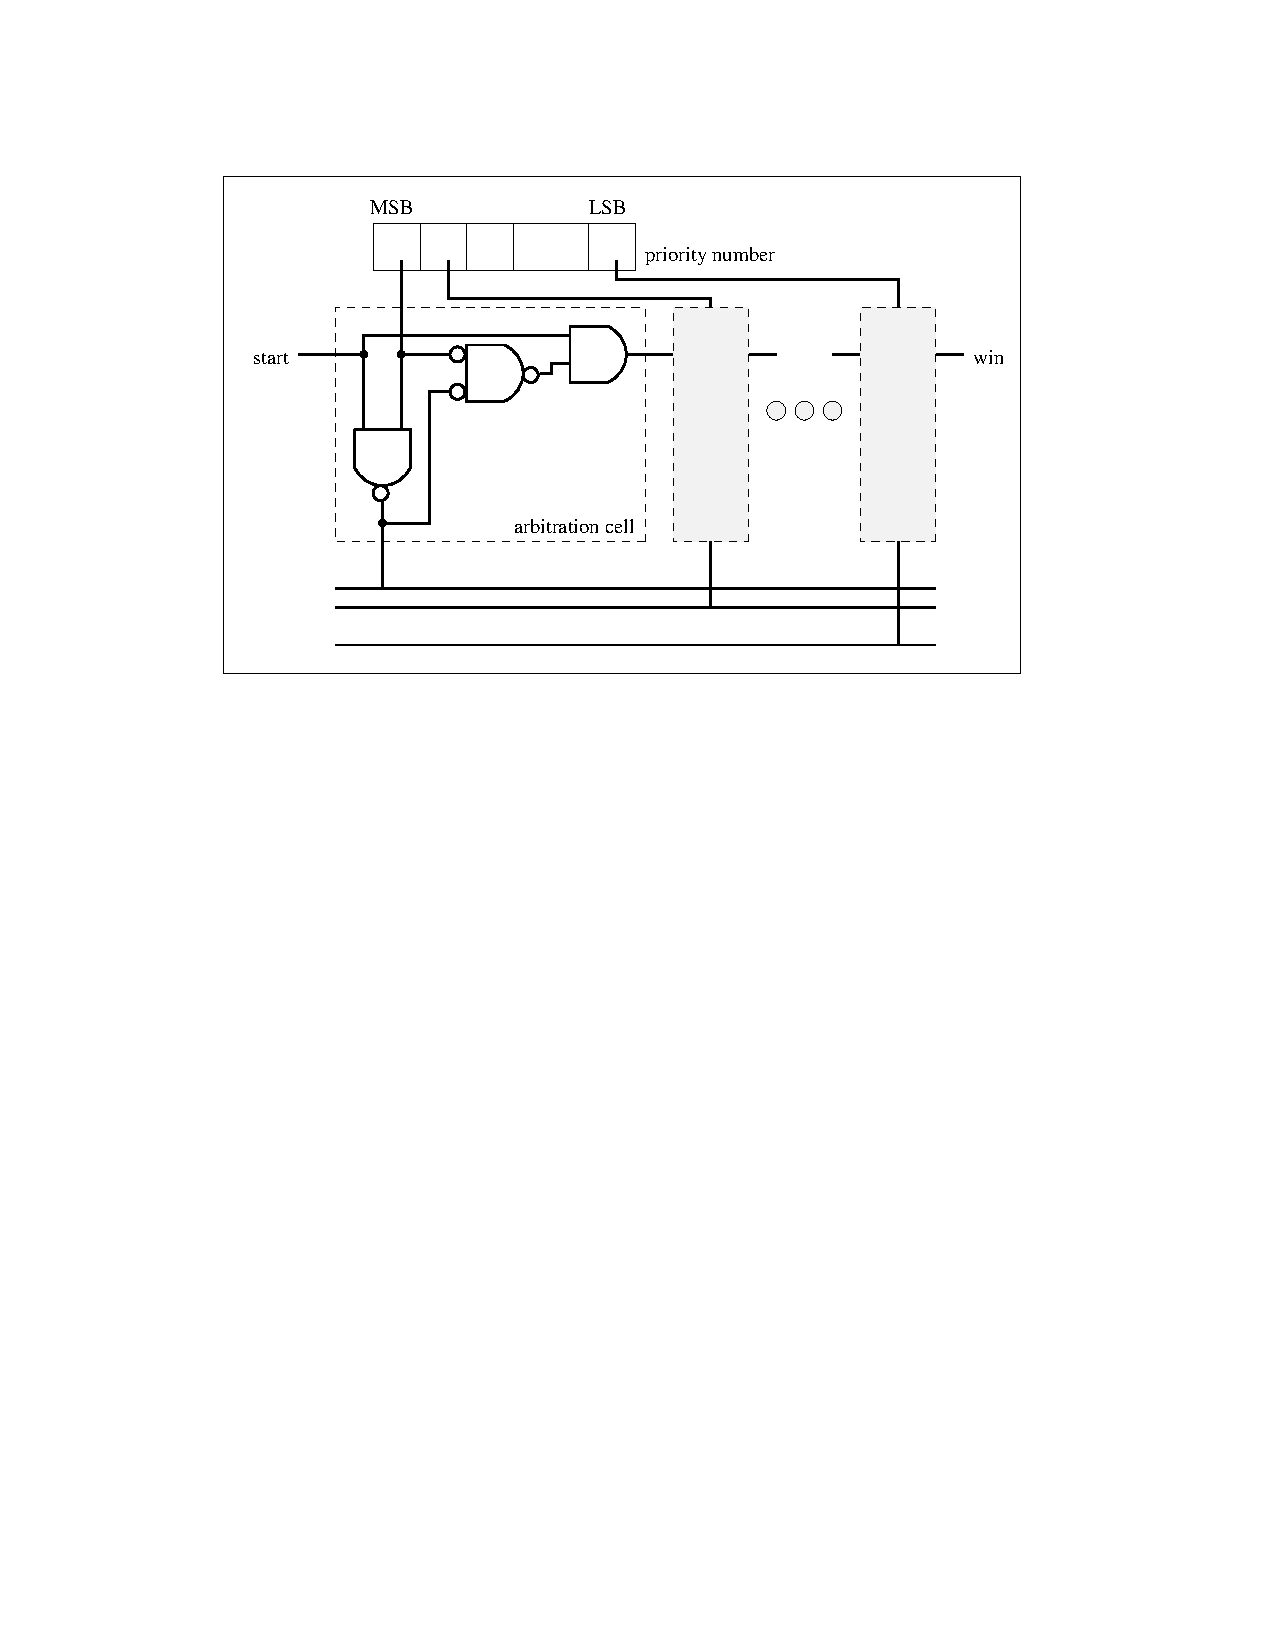
\includegraphics{ch4/FIG/int-arbiter.jpg}}
   \caption{부호화된 자가 중재기의 일례}\label{figure:csa}
\end{figure}
%
%

\newpage
%%%%%
%%Title: HiPi+Bus V0.2 Chapter 4 Section 6
%%Creator: Ando Ki
%%CreationDate: April 1992
%%FileName: sec6
%%RelatedFile: ch4
%%%%%
\section{지정 인터럽트}
지정 인터럽트(direct interrupt)란
인터럽트 요청기가 인터럽트를 받을 처리기의 주소를 지정하여 전송하는 것을 의미한다.
일반적으로 지정 인터럽트는 시험 및 고장 진단을 위한 시스템의 제어 (시험, 고장 진단 등), 
에러의 보고 그리고 실시간 응용 등에 사용될 수 있다. \\
지정 인터럽트는 인터럽트 중재가 끝난 바로 다음 주기에서 시작되고, 5 개의 단계 (Phase)로 구성된다.
각 단계는 버스 클럭 주기 동안 수행된다.
5 단계는 중재 주기를 거쳐 사용 허가를 받은 요청기가
인터럽트 처리기의 주소, 요청기의 주소, 인터럽트의 종류 (벡터)를 전송하는 3 단계와
지정된 처리기가 받은 정보에 대한 응답을 준비하고 응답을 보내는 2 단계로 구성된다.
{\tt <}표~\ref{table:dir-int}{\tt >}는 지정 인터럽트의
단계 별 전송되는 정보와 보내는 측과 받는 측 등을 보여주고 있다.
%\documentstyle[a4]{hbook}
%\begin{document}
%
\begin{table}[htbp]
\caption{지정 인터럽트의 단계별 전송 정보}\label{table:dir-int}
   \begin{center}
   \begin{tabular}{|l|l|l|l|} \hline
	phase & transfer information & from & to \\
\hline \hline
	-5 & interrupt class + slot id + id in slot & IR & IR's \\
	-4 & interrupt class + slot id + id in slot & IR & IR's \\
	-3 & interrupt class + slot id + id in slot & IR & IR's \\
	-2 & interrupt class + slot id + id in slot & IR & IR's \\
	-1 & interrupt class + slot id + id in slot & IR & IR's \\ \hline
	0  & interrupt class + destination address  & IR & IH's \\ \hline
	1  & vector type + source address           & IR & IH \\ \hline
	2  & vector                                 & IR & IH \\ \hline
	3  & dummy                                  & -  & - \\ \hline
	4  & acknowledge                            & IH & IR \\ \hline
   \end{tabular}
   \end{center}
\end{table}
%
%\end{document}

그리고 {\tt <}그림~\ref{figure:dir-int}{\tt >}는 실제
인터럽트 버스상에서의 동작을 보이고 있다.
%
\begin{figure}[htb]
    \centerline{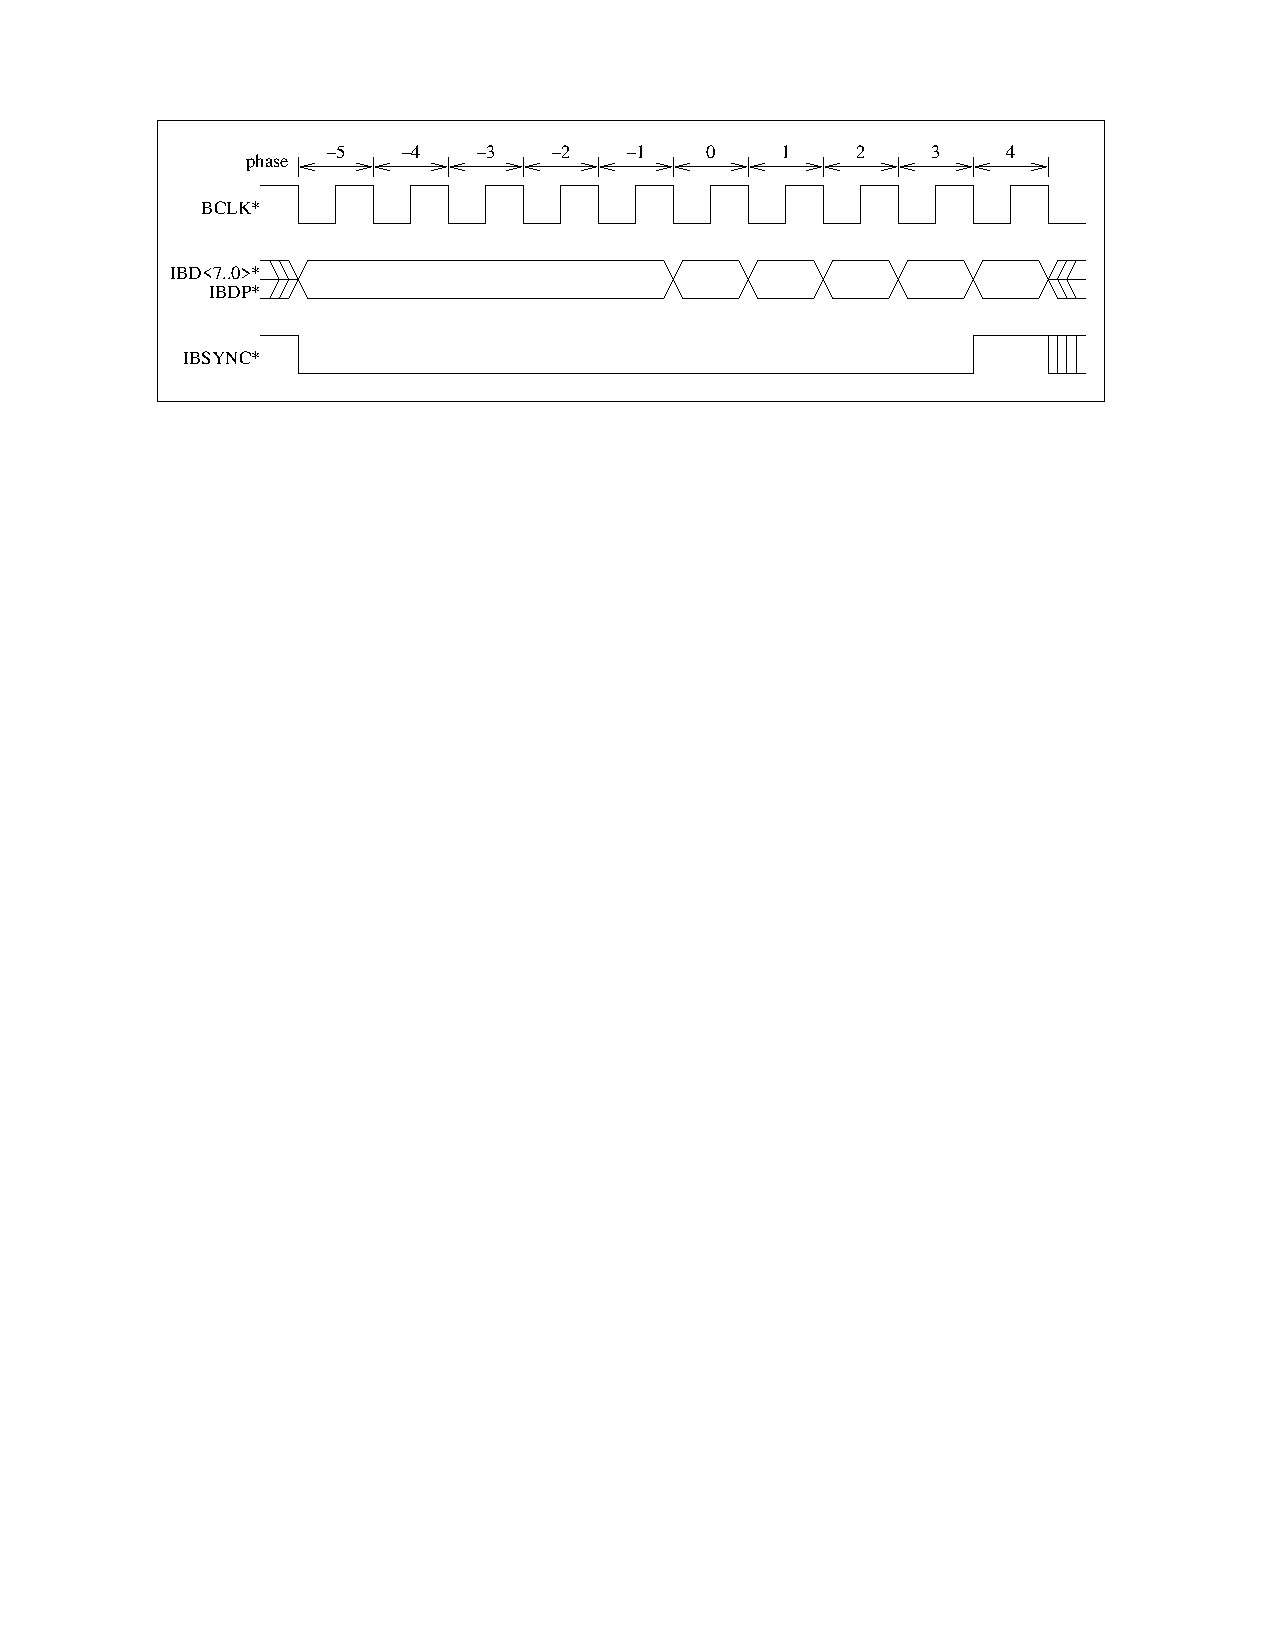
\includegraphics{ch4/FIG/dir-int.jpg}}
   \caption{지정인터럽트의 버스 동작}\label{figure:dir-int}
\end{figure}
%
%
\subsection*{지정 인터럽트 - 단계 -5 --- 단계 -1}
인터럽트 버스를 사용하기에 앞서 수행하는 중재 주기이다.
인터럽트 요청기는 현재 진행 중인 단계가 지정 인터럽트를 보내기에 앞서 수행하는 중재 주기임을
알리기 위해 IBSYNC* 신호를 구동한다.
%
\subsection*{지정 인터럽트 - 단계 0}
이 단계에 전송되는 정보는 종류 정보와 인터럽트를 받는 측(처리기)의 주소가 전송된다.
인터럽트 요청기는 현재 인터럽트 전송이 진행되고 있음을 알리기 위해 IBSYNC* 신호를 구동한다.
비트별 전송 정보는 {\tt <}표~\ref{table:dir-int-p0}{\tt >}과 같다.
%\documentstyle[a4]{hbook}
%\begin{document}
%
\begin{table}[htbp]
\caption{지정 인터럽트 - 단계 0에서 전송되는 정보}\label{table:dir-int-p0}
   \begin{center}
   \begin{tabular}{|l|l|} \hline
	bit field & information \\
\hline \hline
	7, 6 & interrupt class \\ \hline
	5, 4, 3, 2 & slot id \\ \hline
	1, 0 & id in slot \\
\hline
   \end{tabular}
   \end{center}
\end{table}
%
%\end{document}

종류 정보는 지정된 처리기가 저장하게 되는데, 받는 측은 이 값에 따라
다음부터 진행될 단계에 대해서 준비할 수 있게 된다.
종류 필드의 값에 따른 의미는 {\tt <}표~\ref{table:int-class}{\tt >}와 같다. \\
이 단계에서 전송되는 비트 0에서 비트 5까지의 값은 다음 주기부터 전송되는 인터럽트를
받을 처리기의 주소를 나타내는데, 이때 지정된 처리기는 요청기에서 오는 인터럽트 정보를
받고, 해당 동작을 수행하게 된다.
비트 0부터 비트 5까지의 값에 대한 처리기의 할당은 {\tt <}표~\ref{table:ih-ga}{\tt >}과 같다.
Slot ID가 15일 경우는 모든 처리기가 지정된다.
모든 처리기가 지정될 경우, 다음 주기부터 전송되는 정보를 모든 처리기는 동시에 저장하게 된다.
%\documentstyle[a4]{hbook}
%\begin{document}
%
\begin{table}[htbp]
\caption{지정 인터럽트 단계 0의 처리기 어드레스}\label{table:ih-ga}
   \begin{center}
   \begin{tabular}{|l|l|l|} \hline
	Slot ID & ID in Slot & Interrupt Requester \\
\hline \hline
	0 - 12   & x & Slot  0 - Slot 12 \\
	13  - 14 & x & reserved \\
	15 & x & All Handler \\
\hline
   \end{tabular}
   \end{center}
\end{table}
%
%\end{document}

%
\subsection*{지정 인터럽트 - 단계 1}
이 단계에서는 인터럽트 요청기가 처리기에게 벡터의 종류와 자신의 어드레스를 전송한다.
인터럽트 요청기는 현재 인터럽트 전송이 진행 되고 있음을 알리기 위해 IBSYNC* 신호를 구동한다.
처리기의 주소는 6 비트가 사용되고, 상위의 2 비트는 벡터의 종류에 대한 정보를 같이 전송한다.
{\tt <}표~\ref{table:dir-int-p1}{\tt >}는 각 비트별 전송 정보를
나타내고 있다.
\input{ch4/TBL/dir-int-p1}
지정 인터럽트에 의해 전송될 수 있는 벡터의 종류는
{\tt <}표~\ref{table:vec-type}{\tt >}과 같다.
모든 형태의 벡터를 전송할 수 있으나, 최대 전송할 수 있는 벡터의 크기가 8 비트로
한정되어 있기 때문에 16 비트의 벡터를 갖는 경우는 하위 8 비트를 0으로 간주한다.
지정 인터럽트에 의해 전송되는 벡터는 주로 E-와 I-Type이 되며,
시스템의 시험이나 진단을 위한 목적으로 사용된다.
E-Type은 마스크가 불가능하기 때문에 도착한 인터럽트는 항상 해당 프로세서로 전달하고,
I-Type의 경우 마스크되어 있으면 도착한 인터럽트를 무시한다.
Q-와 N-Type은 중재 인터럽트와 동일하게 동작한다 (중재 인터럽트 1 참조).
%
\subsection*{지정 인터럽트 - 단계 2}
이 단계에서는 요청기가 처리기로 인터럽트 벡터(Interrupt Vector)를 보낸다.
인터럽트 요청기는 현재 인터럽트 전송이 진행되고 있음을 알리기 위해 IBSYNC* 신호를 구동한다.
인터럽트 벡터는 요청기가 실질적으로 처리기에 원하는 행동이 무엇인지를 담고 있는 것이다.
인터럽트 벡터는 그들이 갖고 있는 의미에 따라 입출력 동작 제어를 위한 것,
각 슬롯에서 발생된 에러의 보고를 위한 것,
각 슬롯에서 보고된 에러의 처리를 위하여 시스템 콘트롤러에서 보내는 제어를 위한 것,
끝으로 프로세서들 사이에 그들이 수행하고 있는 프로세서 제어나 대화를 위한 정보의
교환을 위한 것등으로 분리할 수 있다.
8 비트의 벡터 값에 따른 의미는 \ref{section:vector-type}에서 설명한 바와 같다.
%
\subsection*{지정 인터럽트 - 단계 3}
인터럽트 요청기는 현재 인터럽트 전송이 진행되고 있음을 알리기 위해 IBSYNC* 신호를 구동한다.
인터럽트를 받은 처리기가 요청기에게 응답을 보내기 위해 이제 까지 받은 정보를 점검하여
다음 단계에서 요청기로 보낼 응답을 준비한다.
%
\subsection*{지정 인터럽트 - 단계 4}
인터럽트 요청기는 현재 진행 중인 단계가 지정 인터럽트의 마지막임을 알리기 위해 이제까지
구동하고 있던 IBSYNC* 신호를 걷어낸다.
지정 인터럽트의 최종 단계로, 인터럽트를 받은 처리기가 요청기에게 응답을 보내는 일을 수행한다.
응답 단계에서는 진행된 인터럽트 전송에 에러 발생 여부와 인터럽트 처리기의 상태 등을 전달한다.
{\tt <}표~\ref{table:dir-int-p3}{\tt >}는 전송되는 8 비트의 응답 정보의
각 비트별 의미를 나타내고 있다.
에러가 발생했을 때 해당 비트의 값은 ``거짓''이 된다.
따라서 정확한 순서와 의미로 인터럽트가 전송된 경우는 각 비트의 값이 ``참''이 되도록 하여야만 한다.
%\documentstyle[a4]{hbook}
%\begin{document}
%
\begin{table}[htbp]
\caption{지정 인터럽트 - 단계 3에서 전송되는 정보의 비트별 의미}\label{table:dir-int-p3}
   \begin{center}
   \begin{tabular}{|l|l|} \hline
	bit field & information \\
\hline \hline
	7 & sequence error \\
	6 & parity error \\
	5 & buffer full error \\
	4 & unacceptable error \\
	3 & {\it reserved} \\
	2 & {\it reserved} \\
	1 & {\it reserved} \\
	0 & overwritten error \\
\hline
   \end{tabular}
   \end{center}
\end{table}
%
%\end{document}

\begin{itemize}
	\item 비트 7은 인터럽트 전송 주기 진행에의 에러가 발생했을 경우에 ``거짓''이 되는 비트로
		전송 도중 (DI의 phase4 이나 AI-1의 phase21 제외)에 IBSYNC* 신호가 거짓이
		되었을 경우가 해당된다.
	\item 비트 6은 단계 0, 1 혹은 2에서 전송된 데이터에 패리티 에러가 검출되었을 때 ``거짓''이 된다.
	\item 비트 5는 벡터가 저장될 곳이 다른 인터럽트에 의해 가득찼을 경우에 ``거짓''이 된다.
	\item 비트4는 전송된 벡터를 저장할 수 없는 처리기나 그밖에 정의되지 않은 에러에 의하여
		벡터를 접수할 수 없는 경우에 ``거짓''이 된다.
	\item 비트 0은 처리기에 현재 처리가 지연된 인터럽트(pended interrupt)가 존재했는데 
		새로운 인터럽트가 발생하여 이전 것을 지워지고 새 인터럽트가 저장됐을 경우 ``거짓''이 된다.
\end{itemize}
각 비트는 정의된 상황이 발생했을 경우 ``거짓''이 되도록 함에 따라
처리기가 아무 응답을 안할 경우도 에러로 처리된다. 
또한 두 개 이상의 처리기가 응답을 해야하는 경우(broadcast)에는 한개만이라도 에러가 없다고
응답이 오면 에러가 발생하지 않은 것으로 간주된다.

\newpage
%%%%%
%%Title: HiPi+Bus V0.2 Chapter 4 Section 7
%%Creator: Ando Ki
%%CreationDate: April 1992
%%FileName: sec7
%%RelatedFile: ch4
%%%%%
\section{중재 인터럽트 1}
중재 인터럽트 1(arbitration interrupt 1)은 다중 프로세서 환경의 효과적인
인터럽트 분배를 구현하기 위해 필요한
인터럽트 전송 방법의 한 형태이다. 이 방법은 인터럽트의 동적인 분배를 실현할 수 있으며,
분배 과정에서 프로세서의 불필요한 Context Switching를 막을 수 있도록 구현되어 있다.
다중 프로세서 운영 체제 환경에서 입출력의 제어와 프로세서 사이의 대화 수단 등으로 사용할 수 있다. \\
중재 인터럽트 1은 지정 인터럽트와는 달리 처리기를 지정하지 않고(프로세서의 모임만 지정),
한개 이상의 처리기에 인터럽트를 동시에 전달한 후, 처리기들 끼리 중재를 하여
인터럽트를 접수할 처리기를 하나만 선정하도록 한다.
중재 과정에서 처리기 들은 현재 자신의 상태(상위 프로세서 등의 상태 포함)에 따라
우선 순위 경쟁을 하게 되는데, 그 순간에 인터럽트를 처리하기에 가장 적절한 것이 선정된다. \\
중재 인터럽트 1도 다른 인터럽트와 같이 인터럽트 버스 사용에 관한 중재 주기가 
끝난 바로 다음 주기부터 요청기에 의하여 시작되고, 22 개의 단계로 구성된다.
첫 단계는 인터럽트 종류, 벡터의 종류 그리고 처리기의 모임을 지정하는 정보를 전송하고,
단계1에서는 단계0에서 전달된 정보를 처리기들이 처리하는 시간이고,
단계2부터 단계16까지는 처리기들 사이의 중재가 진행된다.,
단계17에서는 요청기의 어드레스를 전송하고, 단계18과 단계19에서는 16 비트의
벡터를 전송하고, 단계20에서는 응답기가 이제까지 받은 정보에 대한 점검을 하고,
끝으로 단계21에 처리기는 요청기로 받은 인터럽트에 대한 응답을 보낸다. \\
{\tt <}표~\ref{table:arb-int}{\tt >}는 중재 인터럽트 1의
각 단계 별 전송되는 정보와 방향등을 나타내고 있다.
표에서 처리기에 복수로 표현된 것은 여러개의 처리기가 동작에 참여한다는 것을 의미한다.
%\documentstyle[a4]{hbook}
%\begin{document}
%
\begin{table}[htbp]
\caption{중재 인터럽트 1의 단계별 전송 정보}\label{table:arb-int}
   \begin{center}
   \begin{tabular}{|l|l|l|l|} \hline
	phase & transfer information & from & to \\
\hline \hline
	-5 & Interrupt Class + slot id + id in slot & IR & IR's \\
	-4 & Interrupt Class + slot id + id in slot & IR & IR's \\
	-3 & Interrupt Class + slot id + id in slot & IR & IR's \\
	-2 & Interrupt Class + slot id + id in slot & IR & IR's \\
	-1 & Interrupt Class + slot id + id in slot & IR & IR's \\ \hline
	0 & Interrupt Class + Type + Destination Group ID & IR & IH's \\ \hline
	1 & dummy                                         & - & - \\ \hline
	2 & invers num. of Interrupts in Handler & IH's & IH's \\
	3 & invers num. of Interrupts in Handler & IH's & IH's \\
	4 & invers num. of Interrupts in Handler & IH's & IH's \\
	5 & invers num. of Interrupts in Handler & IH's & IH's \\
	6 & invers num. of Interrupts in Handler & IH's & IH's \\ \hline
	7 & invers Priority of Process & IH's & IH's \\
	8 & invers Priority of Process & IH's & IH's \\
	9 & invers Priority of Process & IH's & IH's \\
	10 & invers Priority of Process & IH's & IH's \\
	11 & invers Priority of Process & IH's & IH's \\ \hline
	12 & Slot Address of Handler & IH's & IH's \\
	13 & Slot Address of Handler & IH's & IH's \\
	14 & Slot Address of Handler & IH's & IH's \\
	15 & Slot Address of Handler & IH's & IH's \\
	16 & Slot Address of Handler & IH's & IH's \\ \hline
	17 & Source Address & IR & IH \\ \hline
	18 & Vector 1 & IR & IH \\ \hline
	19 & Vector 0 & IR & IH \\ \hline
	20 & dummy & - & - \\ \hline
	21 & Acknowledge & IH & IR \\ \hline
   \end{tabular}
   \end{center}
\end{table}
%
%\end{document}

그리고 {\tt <}그림~\ref{figure:arb1-int}{\tt >}는 실제
인터럽트 버스상에서의 동작을 보이고 있다.
%
\begin{figure}[htb]
    \centerline{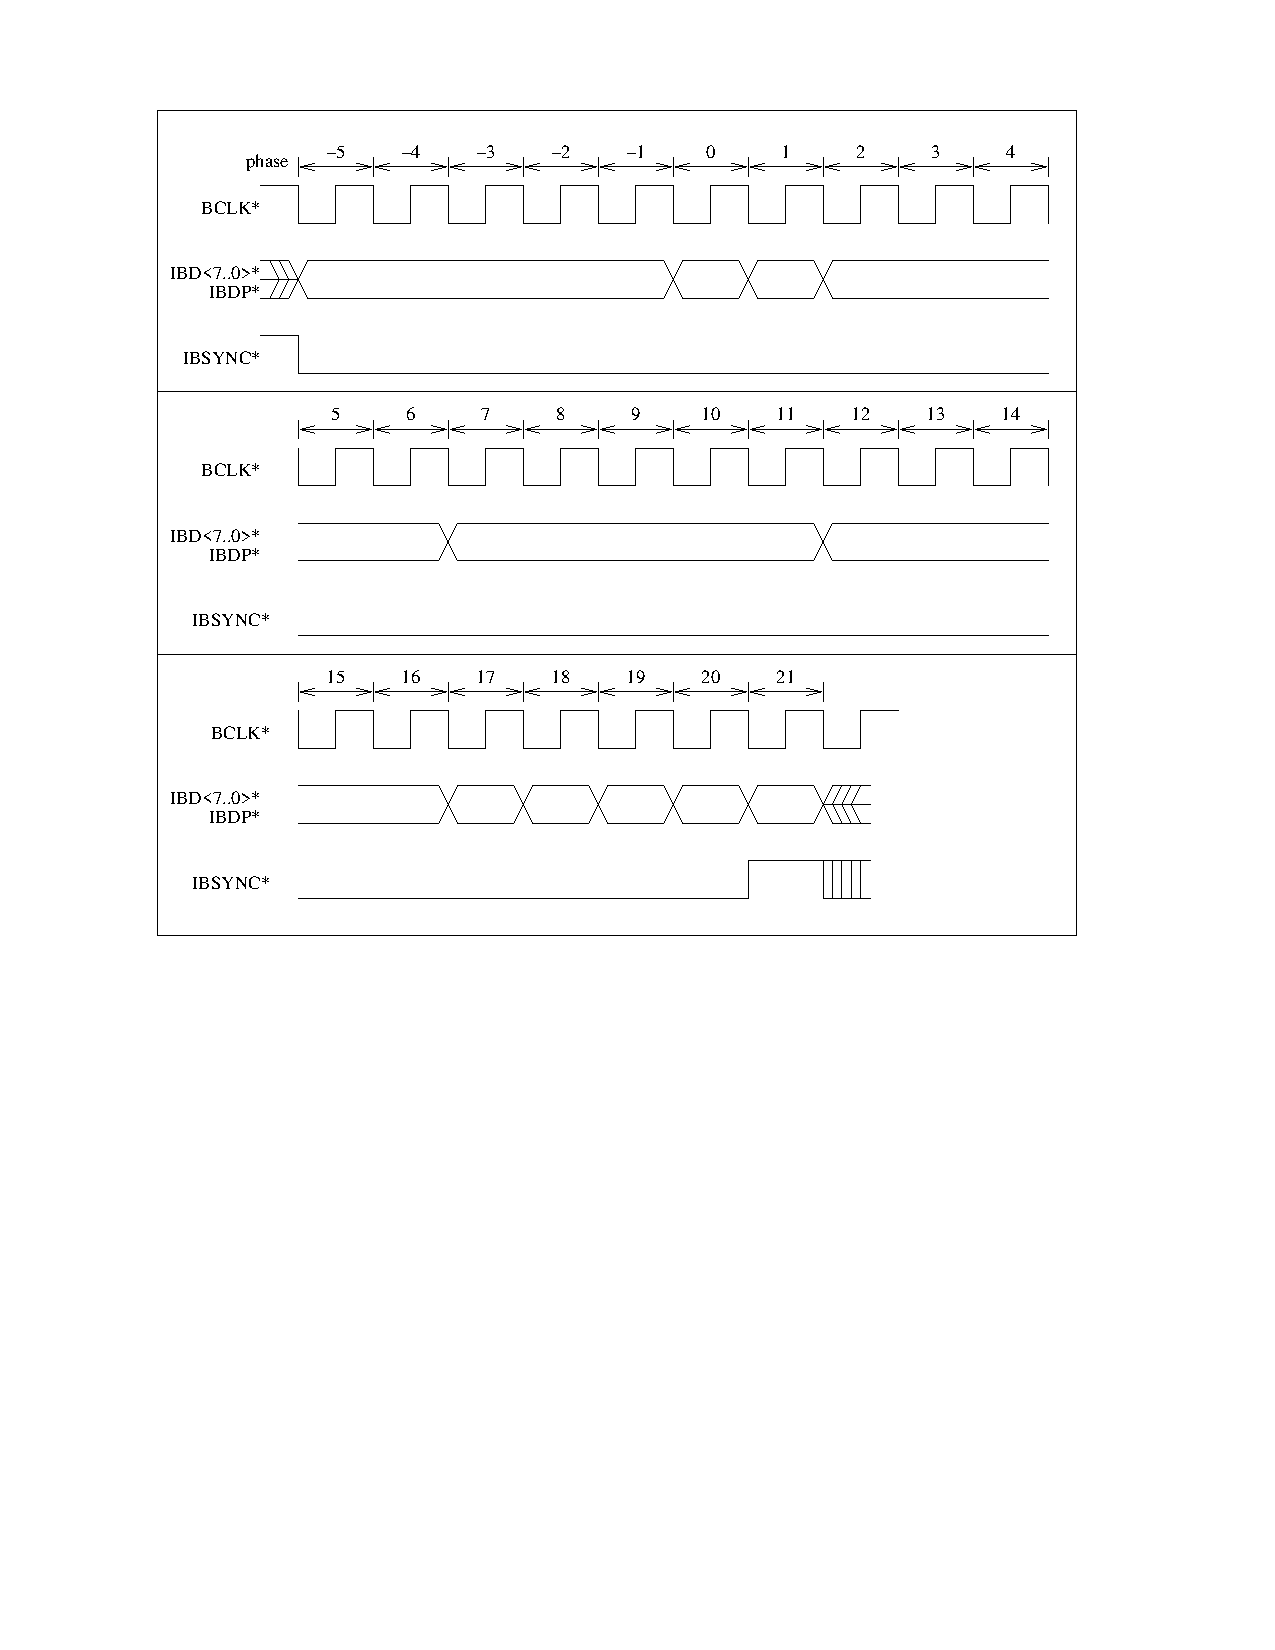
\includegraphics{ch4/FIG/arb1-int.jpg}}
   \caption{중재인터럽트1의 버스 동작}\label{figure:arb1-int}
\end{figure}
%
%
\subsection*{중재 인터럽트 1 - 단계 -5 -- 단계 -1}
인터럽트 버스를 사용하기에 앞서 수행하는 중재 주기이다.
인터럽트 요청기는 현재 진행중인 단계가 중재 인터럽트를 보내기에 앞서 수행하는 중재 주기임을
알리기 위해 IBSYNC* 신호를 구동한다.
%
\subsection*{중재 인터럽트 1 - 단계 0}
인터럽트 요청기는 현재 중재 인터럽트 전송이 진행되고 있음을 알리기 위해 IBSYNC* 신호를 구동한다.
단계 0(phase 0)에서 전송되는 정보는
{\tt <}표~\ref{table:arb-int-p0}{\tt >}과 같이 인터럽트 종류 (Class), 
벡터의 형태 (Type)와 처리기들의 모임 주소 (Group ID)가 전송된다. 
인터럽트 종류 필드는 중재 인터럽트 1을 나타내는 ``2''가 전송된다.
%\documentstyle[a4]{hbook}
%\begin{document}
%
\begin{table}[htbp]
\caption{중재 인터럽트 1 - 단계 0에서 전송되는 정보}\label{table:arb-int-p0}
   \begin{center}
   \begin{tabular}{|l|l|} \hline
	bit field & information \\
\hline \hline
	7, 6 & 2 \\ \hline
	5, 4 & vector type \\ \hline
	3, 2, 1, 0 & group id \\
\hline
   \end{tabular}
   \end{center}
\end{table}
%
%\end{document}

벡터의 종류에 관한 정보가 단계 0에서 전송되는 것이 지정 인터럽트와 다른점으로 볼 수 있다.
벡터의 종류를 단계 0에서 전송하는 이유는 단계 2에서 16까지 진행되는 중재에서
이 정보가 필요하기 때문이다.
중재 인터럽트에서 사용할 수 있는 형태는 {\tt <}표~\ref{table:arb-int-vec}{\tt >}와 같다.
%\documentstyle[a4]{hbook}
%\begin{document}
%
\begin{table}[htbp]
\caption{중재 인터럽트 1의 벡터 형태}\label{table:arb-int-vec}
   \begin{center}
   \begin{tabular}{|l|l|l|} \hline
	type & name & description \\
\hline \hline
	0 & Q-type & queue interrupt \\
	1 & N-type & notify interrupt \\
	2 & AI-1 type-2 & {\it reserved} \\
	3 & AI-1 type-3 & {\it reserved} \\
\hline
   \end{tabular}
   \end{center}
\end{table}
%
%\end{document}

중재 인터럽트의 주된 이용은 다중 처리 운영 체제가 동작하는데 있어서 프로세서들 사이의
동적인 인터럽트의 분배를 위한 것이다. 따라서 벡터 종류도 그와 같은 응용과 밀접한
관계를 갖고 있다. 
\begin{itemize}
	\item N-Type은 notify라는 말이 의미하는 바와 같이 임의의 순간에 발생한 어떤 사건을
	처리기로 통고하는 의미를 지닌다. 따라서 그 인터럽트는 시간과 관계를 갖고 있기 때문에
	시간이 지나면 그 의미를 상실할 수 있다.
	또한 인터럽트가 처리되지 않은 상태에서 또 다시 그 인터럽트가 발생할 경우는
	이와 같은 인터럽트에 해당되는 것은 \ref{section:n-type}에서 설명한 바와 같다.
	\item Q-Type은 한번 전달된 인터럽트는 처리될 때까지 Queue에 저장된다.
	즉 한번 발생된 인터럽트는 무시될 수 없고, 처리가 지연될 수 있으나 무시될 수 없다.
	입출력 인터럽트와 같이 대부분의 인터럽트가 이 형태에 해당된다.
	따라서 인터럽트를 저장할 장소가 없어 인터럽트가 지연될 경우에 새로운 인터럽트가 도착하면
	요청기로 버퍼에 여유가 없음을 알린다.
	처리기에 Queue(FIFO Buffer)를 사용하여 구현하지 않는 경우(오직 한개의 인터럽트만
	저장할 수 있음)는 요청기에서 재시도(retry)를 통해서 Queue의 기능을 대신할 수 있다.
\end{itemize}
%
모임 주소(Group ID)는 처리기들과 연결된 프로세서들을 서로 기능적으로
분류한 주소를 말한다. 본 인터럽트 버스에서는 {\tt <}표~\ref{table:group-id}{\tt >}와 같이
4 종류의 모임을 갖을 수 있고 현재 정의된 주소는 3 개이다.
모임 주소는 비트별로 할당되어 따라서 동시에 2 개 이상의 모임을 선택할 수 있다.
{\tt <}표~\ref{table:group-id}{\tt >}는
모임 주소 각 비트가 지정하는 처리기(해당 프로세서)를 보여 주고 있다.
%\documentstyle[a4]{hbook}
%\begin{document}
%
\begin{table}[htbp]
\caption{중재 인터럽트 1의 모임 주소 각 비트별 의미}\label{table:group-id}
   \begin{center}
   \begin{tabular}{|l|l|} \hline
	group id bit field & group name \\
\hline \hline
	bit 3 & system controllers \\
	bit 2 & input-output processors \\
	bit 1 & {\it reserved} \\
	bit 0 & general purpose processors \\
\hline
   \end{tabular}
   \end{center}
\end{table}
%
%\end{document}

\begin{itemize}
	\item 비트3은 시스템 콘트롤러 그룹을 지정하며, 시스템 제어를 할 수 있는 처리기들이 지정된다.
	\item 비트2는 입출력 처리를 맡고 있는 처리기들이 지정되며, 입출력 프로세서와 시스템 콘트롤러 안에
	입출력 처리 기능을 수행하는 부분에 해당되는 처리기가 지정된다.
	\item 비트0는 일반적인 데이터 처리를 할 수 있는 처리기(프로세서)가 지정된다.
	\item 비트1는 현재 지정되지 않은 것으로 실시간 처리나 그밖의 응용을 위하여 유보하고 있다.
\end{itemize}
각 비트는 어느 조합으로도 동시에 지정이 가능함으로써 3 비트를 동시에 구동하면
시스템 안의 모든 처리기로 중재 인터럽트를 보내게 된다.
%
\subsection*{중재 인터럽트 1 - 단계 1}
인터럽트 요청기는 현재 중재 인터럽트 전송이 진행되고 있음을 알리기 위해 IBSYNC* 신호를 구동한다.
인터럽트 처리기들은 단계 0(phase 0)에서 전송된 정보를 처리한다.
%
\subsection*{중재 인터럽트 1 - 단계 2 --- 단계 6}
인터럽트 요청기는 현재 중재 인터럽트 전송이 진행되고 있음을 알리기 위해 IBSYNC* 신호를 구동한다.
단계 2 (phase 2)부터는 단계 0에서 지정된 처리기들 사이에 수행되는 중재 동작의 첫 단계이다.
처리기들 사이의 중재는 3단계로 구성되는데, {\tt <}표~\ref{table:arb-int}{\tt >}의
단계 2에서 단계 16까지가 해당된다.
지정된 모임 안에 해당되는 처리기들은 각 단계마다 우선 순위 경쟁을 수행하고,
수행한 단계에서 선정된 것들만 계속되는 중재 주기를 수행한다.
결과적으로 단계 16을 마친 후에는 하나의 처리기만 선정되게 된다.
따라서 단계별로 우선 순위가 적용되어 단계 2가 가장 높은 우선 순위 경쟁이 된다. \\
이 단계에서 처리기들이 우선 순위 경쟁을 위해 사용하는 
정보는 처리기 안에 현재 있는 인터럽트 갯수의 역수와 인터럽트 마스크 비트의 
상태
(마스크 되어 있을 경우 0으로 버스에 구동한다) 이다.
%(마스크 되어 있을 경우를
%0으로 함, 즉 가장 높은 우선 순위를 갖는 처리기의 상태는
%모든 비트가 1이 됨)이다. 
이와 같은 중재 정보가 의미하는 것은 마스크가 되어 있지 않을수록, 그리고
처리가 지연되고 있는 인터럽트(Pended Interrupt)가 적은 처리기일수록 
새로운 인터럽트를 접수하는데 있어서 높은 우선 순위를 갖는다는 것이다.
이때 마스크와 인터럽트 갯수는 단계 0에서 지정한 벡터 형태에 관한 것이 된다.
{\tt <}표~\ref{table:arb-int-p2}{\tt >}은 중재 정보로
사용되는 각 데이터의 비트별 할당 상황이다.
%\documentstyle[a4]{hbook}
%\begin{document}
%
\begin{table}[htbp]
\caption{중재 인터럽트 1 - 단계 2에서 사용되는 정보}\label{table:arb-int-p2}
   \begin{center}
   \begin{tabular}{|l|l|} \hline
	bit field & information \\
\hline \hline
	7 & reverse mask bit \\ \hline
	6 & {\it reserved} \\ \hline
	5, 4, 3, 2, 1, 0 & reverse number of interrupts in handler \\
\hline
   \end{tabular}
   \end{center}
\end{table}
%
%\end{document}

%
\subsection*{중재 인터럽트 1 - 단계 7 --- 단계 11}
인터럽트 요청기는 현재 중재 인터럽트 전송이 진행되고 있음을 알리기 위해 IBSYNC* 신호를 구동한다.
단계 7(phase 7)에서는 단계 2의 우선 순위 경쟁에서 이긴 것만 중재를 계속 수행하게 된다.
이 단계에서는 현재 각 처리기에 관련된 프로세서가 수행하고 있는 작업의 우선 순위
(작업의 우선 순위는 운영체제에서 정의한 관리 단위의 수행상 경중을 말함.
UNIX의 경우는 process priority가 이에 해당됨)를 사용하여 중재를 한다.
따라서 새로운 작업을 시작할 때(Context Switching)나 작업의 우선 순위가 변화할 때는
그 우선 순위(Process Priority)를 인터럽트 처리기에 알려주어야 한다.
처리기가 사용할 수 있는 있는 우선 순위는 최대 8 비트이다.
높은 우선 순위를 갖는 작업을 처리하고 있는 프로세서일 경우 이 단계에서 출력되는 정보는
적은 값이 된다.
%\documentstyle[a4]{hbook}
%\begin{document}
%
\begin{table}[htbp]
\caption{중재 인터럽트 1 - 단계 7에서 사용되는 정보}\label{table:arb-int-p7}
   \begin{center}
   \begin{tabular}{|l|l|} \hline
	bit field & information \\
\hline \hline
	7, 6, 5, 4, 3, 2, 1, 0 & inverse priority of process \\
\hline
   \end{tabular}
   \end{center}
\end{table}
%
%\end{document}

%
\subsection*{중재 인터럽트 1 - 단계 12 --- 단계 16}
인터럽트 요청기는 현재 중재 인터럽트 전송이 진행되고 있음을 알리기 위해 IBSYNC* 신호를 구동한다.
단계 12에서도 앞에서와 같이 단계 7까지 우선 순위 경쟁에서 이긴 것들 사이에서만 수행한다.
이 단계에서 사용하는 경쟁 정보는 그 처리기가 현재 위치하는 슬롯 어드레스를 이용한다.
따라서 단계 7까지는 2 개 이상의 처리기가 우선 순위 경쟁에서 이길 수 있으나, 
이 과정을 마치고 나면 항상 1 개의 처리기만이 선정되게 된다.
각 슬롯 어드레스에 대한 위치 배정은 {\tt <}표~\ref{table:arb-int-p12}{\tt >}과 같다.
%\documentstyle[a4]{hbook}
%\begin{document}
%
\begin{table}[htbp]
\caption{중재 인터럽트 1 - 단계 12에서 사용되는 정보}\label{table:arb-int-p12}
   \begin{center}
   \begin{tabular}{|l|l|} \hline
	bit field & information \\
\hline \hline
	7, 6 & 0 \\
	5, 4, 3, 2 & slot id \\
	1, 0 & id in slot \\
\hline
   \end{tabular}
   \end{center}
\end{table}
%
%\end{document}

%
\subsection*{중재 인터럽트 1 - 단계 17}
인터럽트 요청기는 현재 중재 인터럽트 전송이 진행되고 있음을 알리기 위해 IBSYNC* 신호를 구동한다.
이 단계에서는 요청기가 선정된 하나의 처리기로 자신의 주소를 전송한다.
전송되는 정보의 각 비트별 할당은 지정 인터럽트의 단계 1과 같은데,
단지 비트 6과 7을 사용하지 않은 점이 다르다. 이단계에서 사용하는 정보는
{\tt <}표~\ref{table:arb-int-p17}{\tt >}과 같다.
%\documentstyle[a4]{hbook}
%\begin{document}
%
\begin{table}[htbp]
\caption{중재 인터럽트 1 - 단계 17에서 전송되는 정보}\label{table:arb-int-p17}
   \begin{center}
   \begin{tabular}{|l|l|} \hline
	bit field & information \\
\hline \hline
	7, 6 & 0 \\
	5, 4, 3, 2 & slot id \\
	1, 0 & id in slot \\
\hline
   \end{tabular}
   \end{center}
\end{table}
%
%\end{document}

%
\subsection*{중재 인터럽트 1 - 단계 18}
인터럽트 요청기는 현재 중재 인터럽트 전송이 진행되고 있음을 알리기 위해 IBSYNC* 신호를 구동한다.
단계 18에서는 요청기가 처리기로 16 비트의 인터럽트 벡터 중 상위 8 비트를 전송한다.
인터럽트 벡터의 의미는 \ref{section:vector-type}에서 설명한 바와 동일하다.
\input{ch4/TBL/arb-int-p18}
%
\subsection*{중재 인터럽트 1 - 단계 19}
인터럽트 요청기는 현재 중재 인터럽트 전송이 진행되고 있음을 알리기 위해 IBSYNC* 신호를 구동한다.
단계 19에서는 요청기가 처리기로 16 비트의 인터럽트 벡터 중 하위 8 비트를 전송한다.
인터럽트 벡터의 의미는 \ref{section:vector-type}에서 설명한 바와 동일하다.
%\documentstyle[a4]{hbook}
%\begin{document}
%
\begin{table}[htbp]
\caption{중재 인터럽트 1 - 단계 19에서 전송되는 정보}\label{table:arb-int-p19}
   \begin{center}
   \begin{tabular}{|l|l|} \hline
	bit field & information \\
\hline \hline
	7, 6, 5, 4, 3, 2, 1, 0 & lest significant byte of interrupt vector \\
\hline
   \end{tabular}
   \end{center}
\end{table}
%
%\end{document}

%
\subsection*{중재 인터럽트 1 - 단계 20}
인터럽트 요청기는 현재 중재 인터럽트 전송이 진행되고 있음을 알리기 위해 IBSYNC* 신호를 구동한다.
인터럽트 요청기는 이제까지 받은 정보에 대해 점검하고 다음 단계에 사용할 응답을 준비한다.
%
\subsection*{중재 인터럽트 1 - 단계 21}
인터럽트 요청기는 현재 진행 중인 단계가 중재 인터럽트의 마지막임을 알리기 위해 이제까지
구동하고 있던 IBSYNC* 신호를 걷어낸다.
단계 7에서는 인터럽트 처리기가 인터럽트를 보낸 요청기로 응답을 보내는 단계이다.
이 단계에서 전송되는 신호의 의미는 지정 인터럽트의 경우와 동일하며,
{\tt <}표~\ref{table:dir-int-p3}{\tt >}과 같다.
%%

\newpage
%%%%%
%%Title: HiPi+Bus V0.2 Chapter 4 Section 8
%%Creator: Ando Ki
%%CreationDate: April 1992
%%FileName: sec8
%%RelatedFile: ch4
%%%%%
\section{중재 인터럽트 0}
중재 인터럽트 0(arbitration interrupt 0)은 현재 16 단계만 확정되어 있고
앞으로의 확장을 위하여 규격 결정을 유보하고 있다.
%%

\newpage
%%%%%
%%Title: HiPi+Bus V0.2 Chapter 4 Section 8
%%Creator: Ando Ki
%%CreationDate: April 1992
%%FileName: sec9
%%RelatedFile: ch4
%%%%%
\section{예외 처리 (Exception Handling)}
본 절에서는 인터럽트 버스 상에서 동작 중에 앞에서 정의되지 않은 상태가 발생했을 때
처리하는 방법에 대해 기술한다.

\subsection{전송 에러 (Transmission Error)}
인터럽트 전송 주기 안에서 처리기가 패리티 에러를 검출한 경우를 말한다.
처리기는 응답 단계를 통하여 요청기로 전송 중에 에러가 발생했음을 통고하고,
받은 인터럽트는 등록하지 않는다. 요청기는 전송 에러를 받으면
중재 주기 부터 다시 인터럽트 전송을 재시도 (Retry)한다.
재시도한 전송 주기에서 다시 동일한 에러를 검출할 경우는 고장이 발생했음을
시스템 콘트롤러에 전달하고 그 이후의 동작은 버스 규격에서 제시하지 않는다.

%%%%%

%%%%%
%%Title: HiPi+Bus V0.2 Chapter 5
%%Creator: Ando Ki
%%CreationDate: April 1992
%%FileName: ch5
%%RelatedFile: sec1 sec2
%%%%%
\chapter{유틸리티 버스}
%
%%%%%
%%Title: HiPi+Bus V0.2 Chapter 5
%%Creator: Ando Ki
%%CreationDate: April 1992
%%FileName: sec1
%%RelatedFile: ch5
%%%%%
\section{개요}
유틸리티 버스(utility bus)는 버스의 기능을 수행하기 위해 기본적으로
필요한 신호과 버스의 부가적인 기능을 구현하기 위해 추가된 신호들의 집합이다.
%
%\documentstyle[a4]{hbook}
%\begin{document}
%
\begin{table}[htbp]
\caption{유틸리티 버스의 규격 요약}\label{table:ub-spec}
   \begin{center}
   \begin{tabular}{|l l|} \hline
	\multicolumn{2}{|c|}{버스 클럭 (Bus Clock)} \\
\hline
	클럭의 속도 & 16.5 MHz (60.6 {\it n\/}sec) \\
\hline
	\multicolumn{2}{|c|}{버스 제어를 위한 신호} \\
\hline
	슬롯 위치 식별용 & Geographical Slot Address \\
	시스템 제어 용 & System Fail, Reset \\
	경계주사 용 & JTAG Boundary Scan \\
\hline
	\multicolumn{2}{|c|}{기 타 (Etc.)} \\
\hline
	총 신호수 & 13\\ \hline
   \end{tabular}
   \end{center}
\end{table}
%
%\end{document}

%
%%%%%

\newpage
%%%%%
%%Title: HiPi+Bus V0.2 Chapter 5
%%Creator: Ando Ki
%%CreationDate: April 1992
%%FileName: sec2
%%RelatedFile: ch5
%%%%%
\section{유틸리티 버스의 신호선}
%
%\documentstyle[a4]{hbook}
%\begin{document}
%
\begin{table}[htbp]
\caption{유틸리티 버스의 신호들}\label{table:ub-signal}
   \begin{center}
   \begin{tabular}{|l|r|l|} \hline
	Mnemonic & Size & Name \\
\hline \hline
	BCLK*		& 1 & Bus Clock \\
	GA$<$4..0$>$*   & 5 & Geographical Slot Address \\
	SFAIL*          & 1 & System Fail \\
	RST*            & 1 & Reset \\
	Tx$<$4..0$>$	& 5 & JTAG Boundary Scan Option \\ \hline
   \end{tabular}
   \end{center}
\end{table}
%
%\end{document}

%
\subsection*{Bus Clock : BCLK*}
버스 동작의 기준 시간이 되는 신호이다. 백플레인에서 공급된다.
각 슬롯에 도착되는 신호의 시간 차이 발생을 최소화하기 위하여
두개의 슬롯씩 별도의 신호를 두어 클럭을 공급한다. 단 슬롯 10번은
슬롯 8, 슬롯  9와 같이 연결된다.
%
\subsection*{Geographical Slot Address : GA$<$4..0$>$*}
슬롯 어드레스는 슬롯의 위치를 나타내는 5 비트의 신호들로써 슬롯에 삽입된 보드는
이 신호를 통하여 자신의 위치를 알 수 있게 된다.
슬롯의 어드레스는 주서브랙(main sub-rack)의 전면에서 볼 때 가장 왼쪽이 슬롯 0가 되고, 
순서적으로 할당되어 가장 오른쪽이 슬롯 20이 된다.
각 슬롯마다 독립적으로 자신의 위치를 나타내는 값을 버스 콘넥터에 제공해야 하므로
다른 버스의 신호와 달리 모든 슬롯을 연결시키는 신호가 아니다.
$<$표~\ref{table:ga}$>$은 보드가 꽂히는 쪽(백플레인의 전면)에서 바라본 슬롯의 위치와
슬롯 어드레스 값의 대응관계를 보여 주고 있다.
%
%\documentstyle[a4]{hbook}
%\begin{document}
%
\begin{table}[htbp]
\caption{슬롯 어드레스와 슬롯 위치}\label{table:ga}
   \begin{center}
   \begin{tabular}{|l|l l l l l l l l l c l l l l l l l l|} \hline
	Slot No. & 0&1&2&3&4&5&6&7&8&...&13&14&15&16&17&18&19&20 \\
\hline \hline
	GA{\tt <}4{\tt >}* &0&0&0&0&0&0&0&0&0&...&0&0&0&1&1&1&1&1 \\
	GA{\tt <}3{\tt >}* &0&0&0&0&0&0&0&0&1&...&1&1&1&0&0&0&0&0 \\
	GA{\tt <}2{\tt >}* &0&0&0&0&1&1&1&1&0&...&1&1&1&0&0&0&0&1 \\
	GA{\tt <}1{\tt >}* &0&0&1&1&0&0&1&1&0&...&0&1&1&0&0&1&1&0 \\
	GA{\tt <}0{\tt >}* &0&1&0&1&0&1&0&1&0&...&1&0&1&0&1&0&1&0 \\
\hline
   \end{tabular}
   \end{center}
\end{table}
%
%\end{document}

%
각 슬롯에 꽂히는 보드들은 초기화 과정에서 이 슬롯 어드레스를 읽어서 중재 번호, 인터럽트 버스의
인터럽트 요청기와 처리기의 주소, 그리고 기타 자신을 나타내는 번호(ID)로 사용한다.
%
\subsection*{System Reset : RST*}
시스템 전원을 올린 후 시스템 내의 모든 하드웨어의 초기화를 위하여 사용하며, 또한 시스템의 운영중
복구가 불가능한 에러가 발생했을 경우에도 하드웨어의 초기화를 위하여 사용한다.
시스템 콘트롤러에 의해서 구동되고 다른 모든 슬롯에 위치하는 모듈은 입력 신호로 사용된다.
이 신호가 구동될 경우 각 모듈은 수행 중인 작업을 중단하고 자신이 갖고 있는 모든 자원을 
초기화하여야 한다. 이 신호의 시간 규격은 최소한 100 {\it m\/}sec
동안 안정한 값을 구동하여야 한다는 것이다.
%
\subsection*{System Fail : SFAIL*}
시스템의 고장 신호는 국부적으로 복구가 불가능한 시스템의 고장이 발생했을 때, 시스템 콘트롤러에 고장의 발생을
알리는 신호로 사용된다. 보통 복구가 불가능한 에러는 동시에 여러 슬롯에서 발생할 수 있기 때문에
두개 이상의 모듈이 동시에 구동이 가능하다.
%
\subsection*{Boundary Scan Option : Tx$<$4..0$>$}
JTAG (Joint Test Action Group) 경계주사(boundary scan) 기능을
위한 핀이다. 정확한 기능과 규격은 IEEE Std.1149.1을 따르며 여기에서는
$<$표~\ref{table:jtag}$>$과 같이 사용핀을 정의한다.
%\documentstyle[a4]{hbook}
%\begin{document}
%
\begin{table}[htbp]
\caption{경계주사}\label{table:jtag}
   \begin{center}
   \begin{tabular}{|l|l|l|} \hline
	& define & description \\
\hline \hline
	Tx{\tt <}4{\tt >} & TRST* & Test Reset Input \\
	Tx{\tt <}3{\tt >} & TDO   & Test Data Out \\
	Tx{\tt <}2{\tt >} & TDI   & Test Data Input \\
	Tx{\tt <}1{\tt >} & TMS   & Test Mode Select Input \\
	Tx{\tt <}0{\tt >} & TCK   & Test Clock Input \\
\hline
   \end{tabular}
   \end{center}
\end{table}
%
%\end{document}

%
%

%%%%%

%%%%%
%%Title: HiPi+Bus V0.2 Chapter 6
%%Creator: Ando Ki
%%CreationDate: April 1992
%%FileName: ch6
%%RelatedFile:
%%%%%
\chapter{시간 규격}
%
%%%%%
%%Title: HiPi+Bus V0.2 Chapter 6
%%Creator: Ando Ki
%%CreationDate: April 1992
%%FileName: sec1
%%RelatedFile: ch6
%%%%%
\section{개요}
시간규격에서는  백플레인에 구동되는 신호의 시간적 제약을 규정한다.
모든 시간규격은 백플레인에 나타나는 실제 신호를 기준으로 표시하며, 표시의 편의를 위해
토템폴 신호, 트라이스테이트 신호 그리고 오픈콜렉터 신호를 따로 구분하지 않고,
여러 신호가 모여서 동작하는 신호와 단일 신호를 따로 구분하지 않는다.
각 시간규격은 버스의 부하에 관계없이 최소값과 최대값의 범위를 넘지 않아야한다.

전달지연시간(propagation time)은 구동소자의 출력단 신호가
변하기 시작하여 백플레인에 나타나는 신호가 백플레인의 모든 곳에서
전기적규격에서 규정하는 $V_{OL}$ 이하로 안정될 때까지의 시간으로 규정한다.\footnote{BTL의 경우
90\%에서 10\%로의 하강시간이 최대 10$n$sec이고, 백플레인의 슬롯이 0.8inch 간격으로
21개 있을 때 5$n$sec/ft 이내의 전달 지연을 보장하면 신호가 백플레인을 최장으로 전달된다해도
10$n$sec 이내의 지연이 보장되므로 HiPi+Bus에서는 버스 전달 지연(bus propagation
time)을 최대 20$n$sec로 규정한다.}
%

\newpage
%%%%%
%%Title: HiPi+Bus V0.2 Chapter 6
%%Creator: Ando Ki
%%CreationDate: April 1992
%%FileName: sec2
%%RelatedFile: ch6
%%%%%
\section{버스클럭의 시간규격}
%
버스 클럭 신호는 본 시스템 버스의 모든 부분의 제어에 있어서 기준이 되는 신호이다.
클럭은 슬롯 10에서 공급되고 다른 슬롯에 위치한 모든 보드들은 이 신호를 받아서 제어 정보로 사용한다.
%
%\documentstyle[a4]{hbook}
%\begin{document}
%
\begin{table}[htbp]
\caption{버스클럭의 시간규격 요약}\label{table:bclk-time}
   \begin{center}
   \begin{tabular}{|l|l|r|r|r|} \hline
	timing parameter & name & min & typical & max \\ \hline \hline
	$TP^{BCLK}_0$ & BCLK* cycle time & 59 & 60 & 61 \\ \hline
	$TP^{BCLK}_1$ & BCLK* high pulse width & - & 30 & - \\ \hline
	$TP^{BCLK}_2$ & BCLK* low pulse width & - & 30 & - \\ \hline
	$TP^{BCLK}_3$ & BCLK* falling transition time & 3 & - & 5 \\ \hline
   \end{tabular}
   \end{center}
\end{table}
%
%\end{document}

\begin{figure}[htb]
    \centerline{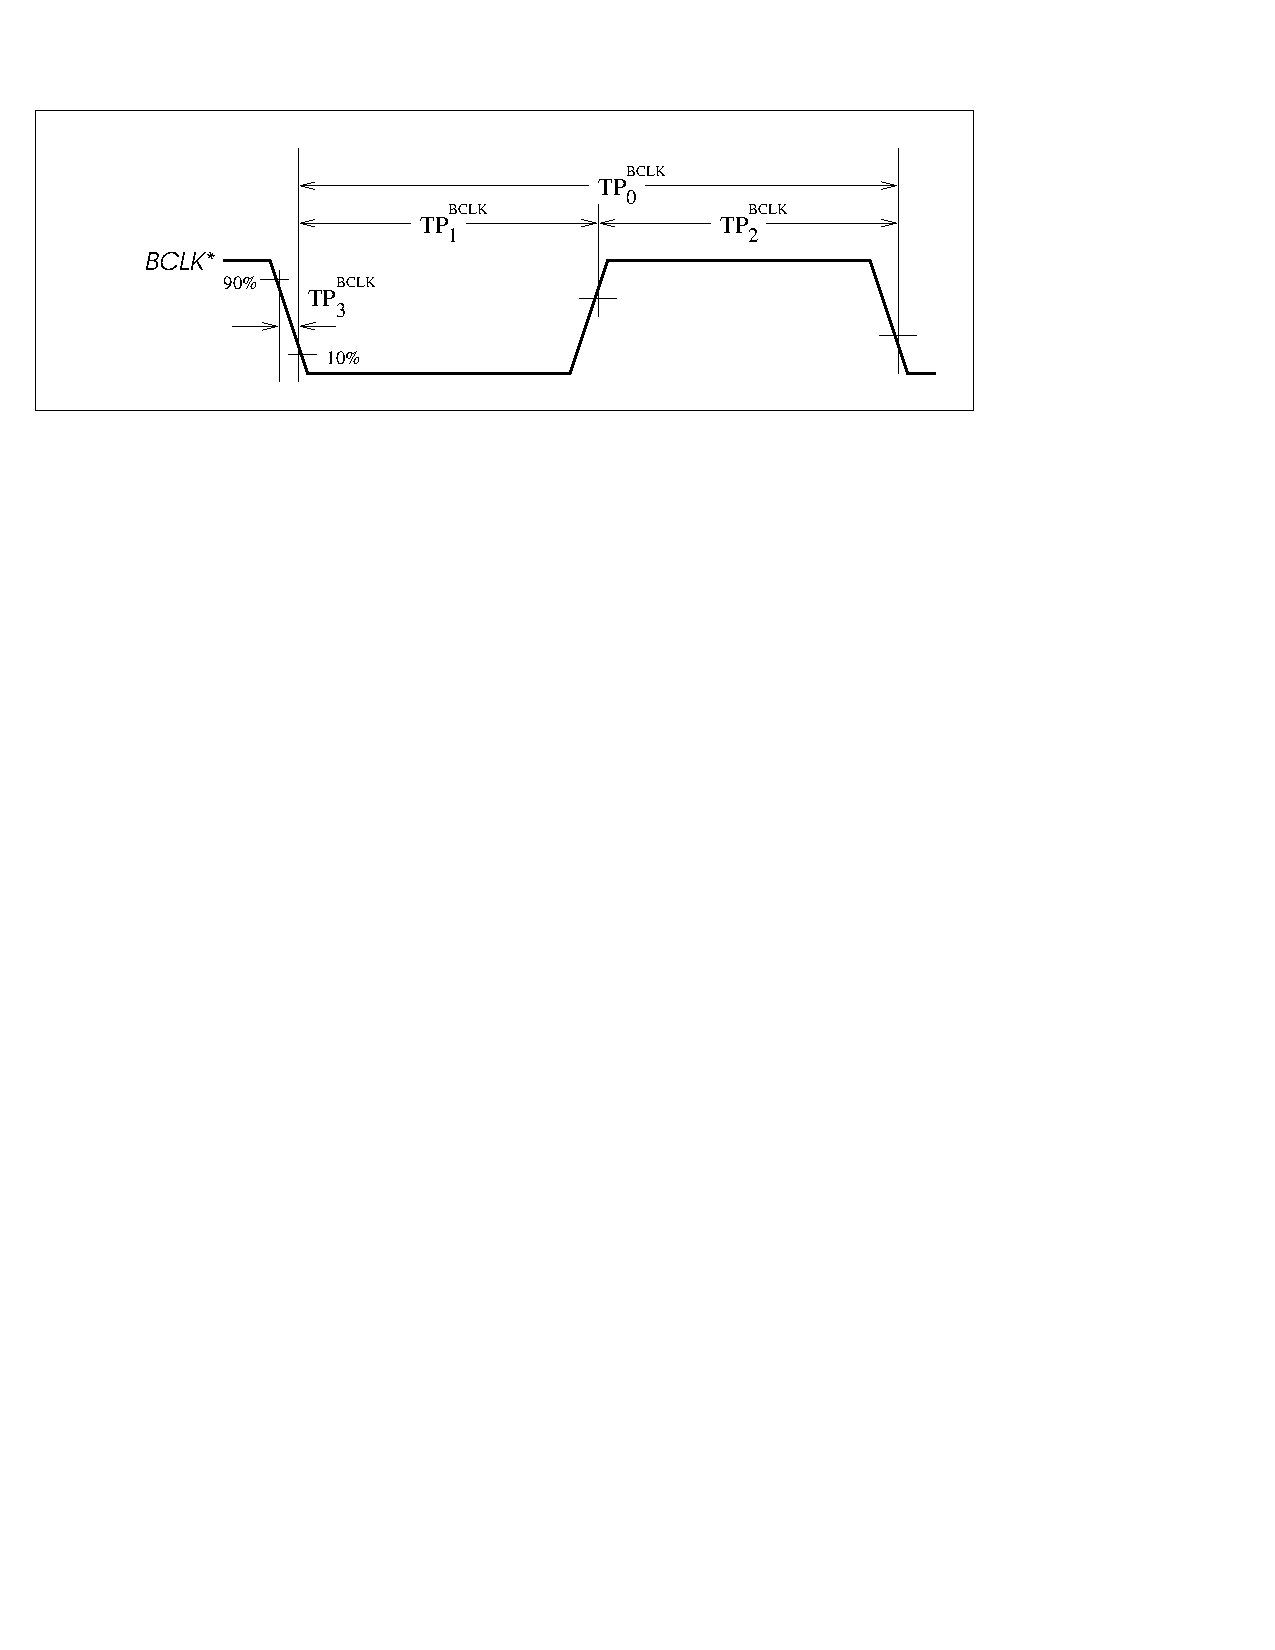
\includegraphics{ch6/FIG/bclk-time.jpg}}
   \caption{버스클럭의 시간규격}\label{figure:bclk-time}
\end{figure}
%

버스클럭의 속도(clock frequency)는 16.5 MHz로
60.6 $n$sec의 주기(clock period, clock cycle time))를
갖으며 정확한 제어를 위하여 
백플레인에 나타나는 버스클럭 신호의 하강점(falling edge)만을
사용하도록 규정하고 시간적 허용오차는 $\pm1 n$sec 이내로 규정한다.
클럭의 Duty Cycle은 50\% ($TP^{BCLK}_1 \div TP^{BCLK}_0$)로 규정한다.
버스클럭 신호가 90\%에서 10\%로 
천이하는 시간인 하강점 천이시간(falling transition time)를
3 $n$sec 이상 5 $n$sec 이내로 규정한다.
%%%%%

\newpage
%%%%%
%%Title: HiPi+Bus V0.2 Chapter 6
%%Creator: Ando Ki
%%CreationDate: April 1992
%%FileName: sec3
%%RelatedFile: ch6
%%%%%
\section{중재버스의 시간규격}
\subsection{ABRQ{\tt <}n{\tt >}*, DBRQ{\tt <}n{\tt >}*의 시간규격}
중재에 참가하기 위해서는 중재에 참가하고자 하는 버스클럭 주기에
해당 버스클럭의 백플레인의 하강점에서 $TP^{ARB}_1$ 시간 이후부터
$TP^{ARB}_0$ 동안 해당 중재요청신호를 백플레인에 안정되게 구동하여야 한다.
이때 중재요청신호의 전달지연시간은 $TP^{ARB}_2$로 규정한다.
중재 주기에서 중재를 수행한 결과 버스 사용권을 획득한 중재기는 자신의 중재요청신호의
구동을 이어지는 중재에 여향을 미치지 않도록 충분히 빨리 신호구동을 멈추어야 하고
이때 $TP^{ARB}_3$를 보장하여야 한다.
나머지 중재기들은 중재요청신호를 계속 구동하여 이어진 중재주기로 중재동작을 계속하게 된다.
%\documentstyle[a4]{hbook}
%\begin{document}
%
\begin{table}[htbp]
\caption{중재버스 신호의 시간규격 요약}\label{table:arb-time}
   \begin{center}
   \begin{tabular}{|l|l|r|r|r|} \hline
	timing parameter & name & min & typical & max \\ \hline \hline
	$TP^{BCLK}_0$ & BCLK* cycle time & 59 & 60 & 61 \\ \hline
	$TP^{ARB}_0$  & arbitration time & - & 50 & - \\ \hline
	$TP^{ARB}_1$  & pre-time & - & - & 10 \\ \hline
	$TP^{ARB}_2$  & bus propagation time & - & - & 20 \\ \hline
	$TP^{ARB}_3$  & off time & 10 & - & 15 \\ \hline \hline
	$TP^{INH}_0$  & ABINH time & 25 & 30 & 35 \\ \hline
	$TP^{INH}_1$  & bus propagation time & - & - & 20 \\ \hline
	$TP^{INH}_2$  & off time & 10 & - & 15 \\ \hline
   \end{tabular}
   \end{center}
\end{table}
%
%\end{document}

\begin{figure}[htb]
    \centerline{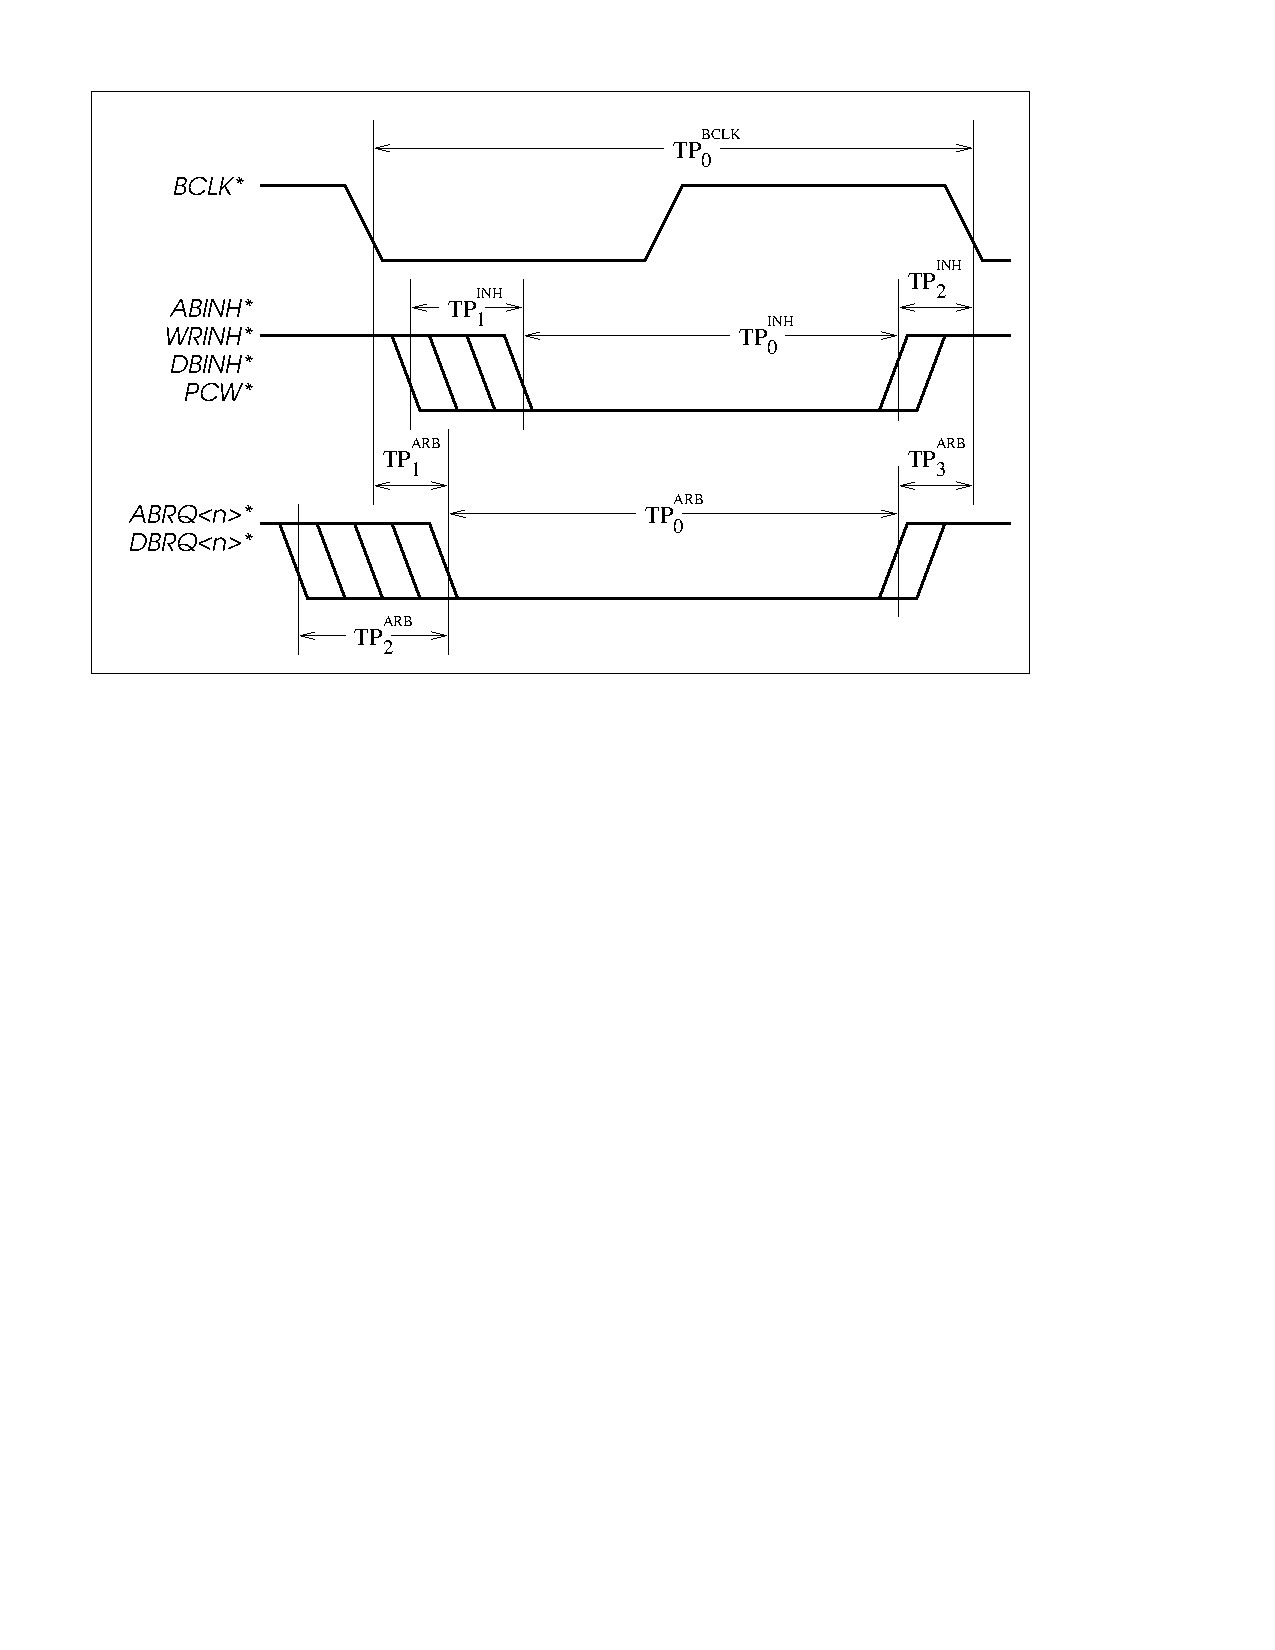
\includegraphics{ch6/FIG/arb-time.jpg}}
   \caption{중재버스의 시간규격}\label{figure:arb-time}
\end{figure}
%
\subsection{ABINH*, WRINH*, DBINH*의 시간규격}
이 신호는 중재요청신호의 구동을 제한하는데 사용하며
$TP^{INH}_0$ 시간동안 안정된 신호로 유지되어야 한다.
연속해서 여러 버스 사이클 동안 구동하는 경우, $TP^{INH}_1$ 시간은 무시하고
처음 구동 사이클에서 지킨다.
연속해서 여러 버스 사이클 동안 구동하는 경우, $TP^{INH}_2$ 시간은 무시하고
마지막 구동 사이클에서 지킨다.
%
%%%%%

\newpage
%%%%%
%%Title: HiPi+Bus V0.2 Chapter 6
%%Creator: Ando Ki
%%CreationDate: April 1992
%%FileName: sec4
%%RelatedFile: ch6
%%%%%
\section{데이터 전송버스의 시간규격}
데이터 전송 버스는 동기형 제어 방식을 사용함에 따라 모든 신호는 한개 클럭 주기 동안에 버스 상에서
구동되고 감지하게 된다. 따라서 모든 신호는 데이터 전송 프로토콜에서 규정된대로
자신에게 할당된 주기에 언제나 한개 버스 클럭 동안만 구동을 하게된다.
%
%\documentstyle[a4]{hbook}
%\begin{document}
%
\begin{table}[htbp]
\caption{데이터 전송 버스 신호의 시간규격 요약}\label{table:dtb-time}
   \begin{center}
   \begin{tabular}{|l|l|r|r|r|} \hline
	timing parameter & name & min & typical & max \\ \hline \hline
	$TP^{BCLK}_0$ & BCLK* cycle time & 59 & 60 & 61 \\ \hline
	$TP^{DTB}_0$  & DTB signal latch point & 38 & 40 & 42 \\ \hline
	$TP^{DTB}_1$  & bus propagation time & - & - & 20 \\ \hline
	$TP^{DTB}_2$  & setup time & 10 & - & - \\ \hline
	$TP^{DTB}_3$  & hold time & 5 & - & - \\ \hline
	$TP^{DTB}_4$  & guard time & 10 & - & - \\ \hline
   \end{tabular}
   \end{center}
\end{table}
%
%\end{document}

\begin{figure}[htb]
    \centerline{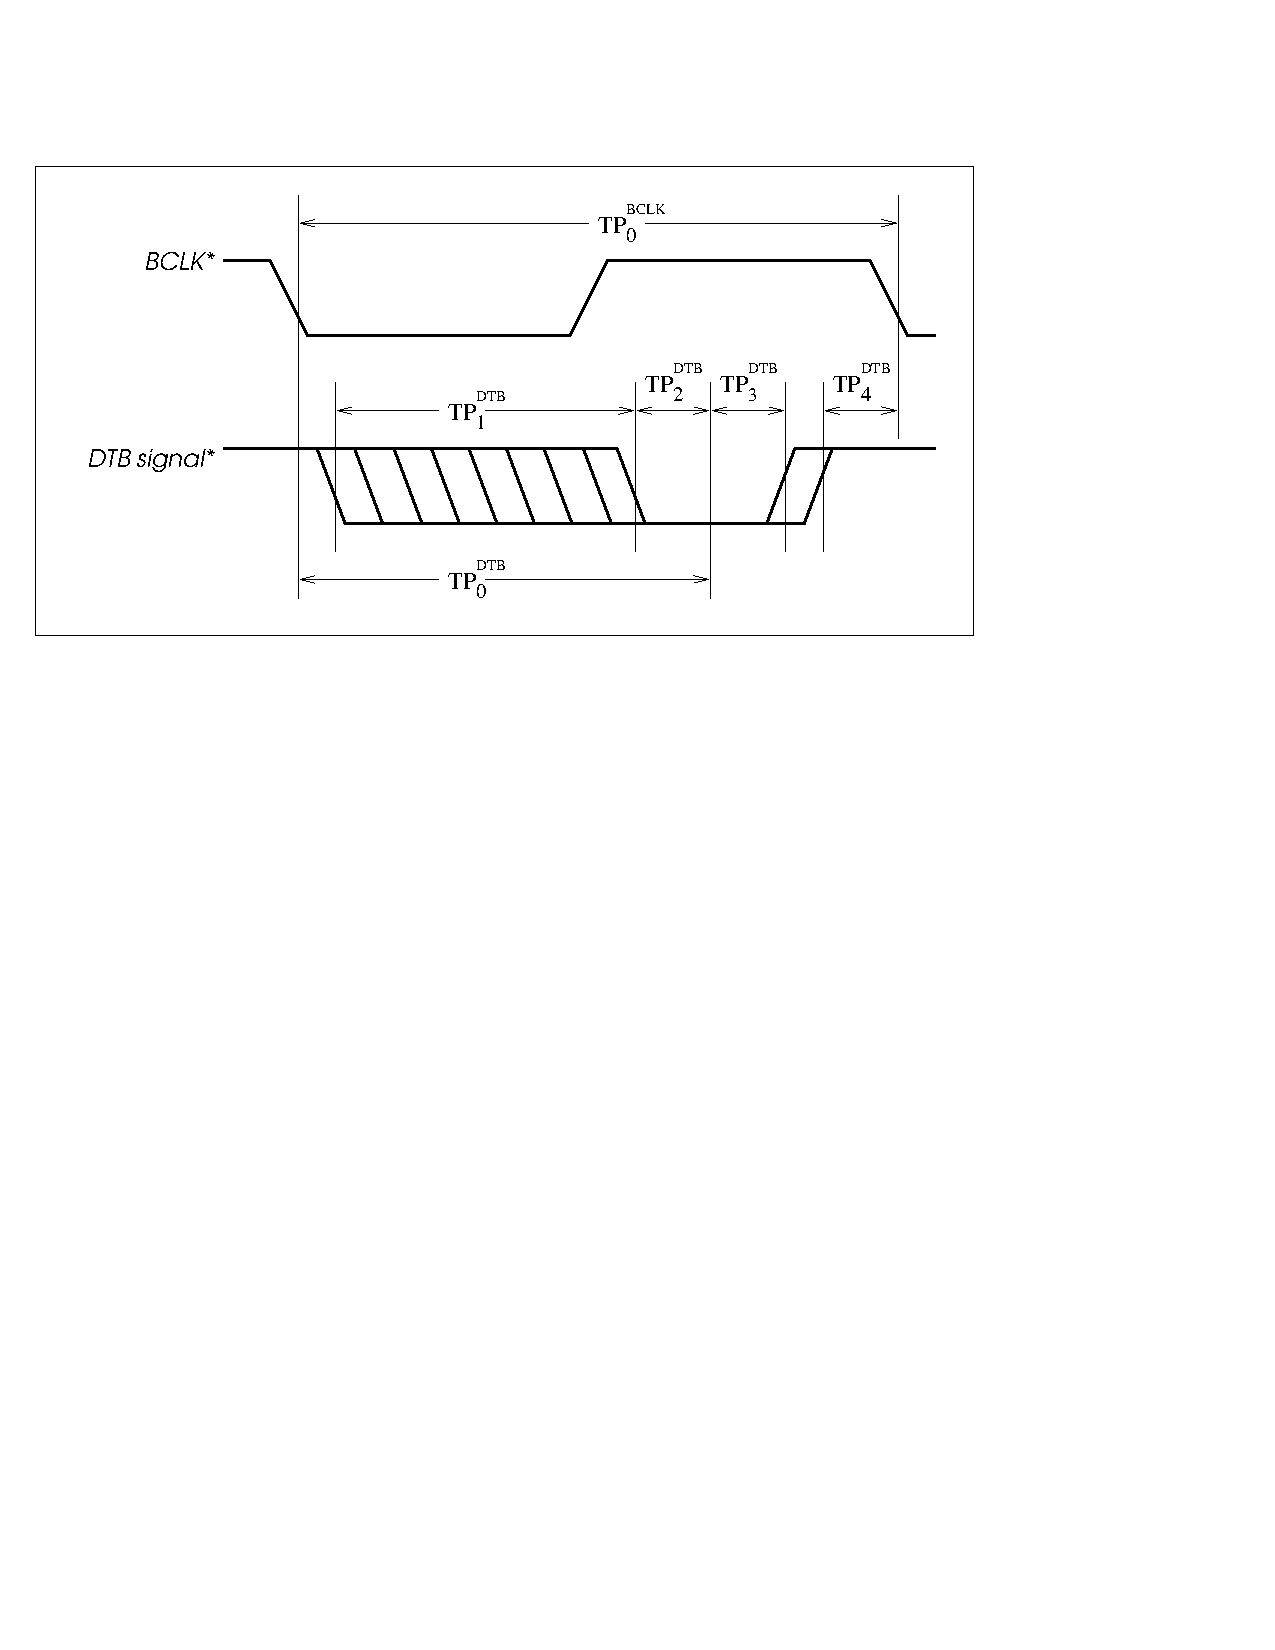
\includegraphics{ch6/FIG/dtb-time.jpg}}
   \caption{데이터 전송버스 신호의 시간규격}\label{figure:dtb-time}
\end{figure}
%

데이터 전송버스의 모든 정보는 백플레인에 나타나는 버스클럭 신호의 하강점으로부터
$TP^{DTB}_0$(DTB signal latch time)후에
데이터 전송버스 정보를 안정되게 래치할 수 있도록 보장해야 한다.
이를 위하여 셋업시간(setup time)으로 $TP^{DTB}_2$를
홀드시간(hold time)으로 $TP^{DTB}_3$를 반드시 보장해야 한다.
그리고 이어지는 버스클럭에 구동될 신호와의 충돌을 방지하기 위해
$TP^{DTB}_4$를 보장해야 한다.
%
%%%%%

\newpage
%%%%%
%%Title: HiPi+Bus V0.2 Chapter 6
%%Creator: Ando Ki
%%CreationDate: April 1992
%%FileName: sec5
%%RelatedFile: ch6
%%%%%
\section{인터럽트버스의 시간규격}
%
\subsection{IBSYNC* 신호의 시간규격}
IBSYNC* 신호는
백플레인에 나타나는 버스클럭의 하강점에서 $TP^{IBSYNC}_0$후에
안정된 신호를 래치할 수 있도록 셋업시간으로 $TP^{IBSYNC}_2$을
홀드시간으로 $TP^{IBSYNC}_3$를 보장해야 한다.
IBSYNC* 신호를 ``거짓(high voltage level)''로 하기 위해서는
구동을 멈추어야 하는데 이때 다음 신호에 영향을 주지 못하도록 $TP^{IBSYNC}_4$을
보장해야 한다. 여러 버스 사이클 동안 구동하는 경우, $TP^{IBSYNC}_1$은
처음 사이클에서, $TP^{IBSYNC}_4$는 마지막 사이클에서만 지키면 된다.
%\documentstyle[a4]{hbook}
%\begin{document}
%
\begin{table}[htbp]
\caption{IBSYNC* 신호의 시간규격 요약}\label{table:ibsync-time}
   \begin{center}
   \begin{tabular}{|l|l|r|r|r|} \hline
	timing parameter & name & min & typical & max \\ \hline \hline
	$TP^{BCLK}_0$   & BCLK* cycle time & 59 & 60 & 61 \\ \hline
	$TP^{IBSYNC}_0$  & IBSYNC* latch point & 38 & 40 & 42 \\ \hline
	$TP^{IBSYNC}_1$  & bus propagation time & - & - & 20 \\ \hline
	$TP^{IBSYNC}_2$  & IBSYNC* setup time & 10 & - & - \\ \hline
	$TP^{IBSYNC}_3$  & IBSYNC* hold time & 5 & - & - \\ \hline
	$TP^{IBSYNC}_4$  & IBSYNC* guard time & 10 & - & - \\ \hline
   \end{tabular}
   \end{center}
\end{table}
%
%\end{document}

\begin{figure}[htb]
    \centerline{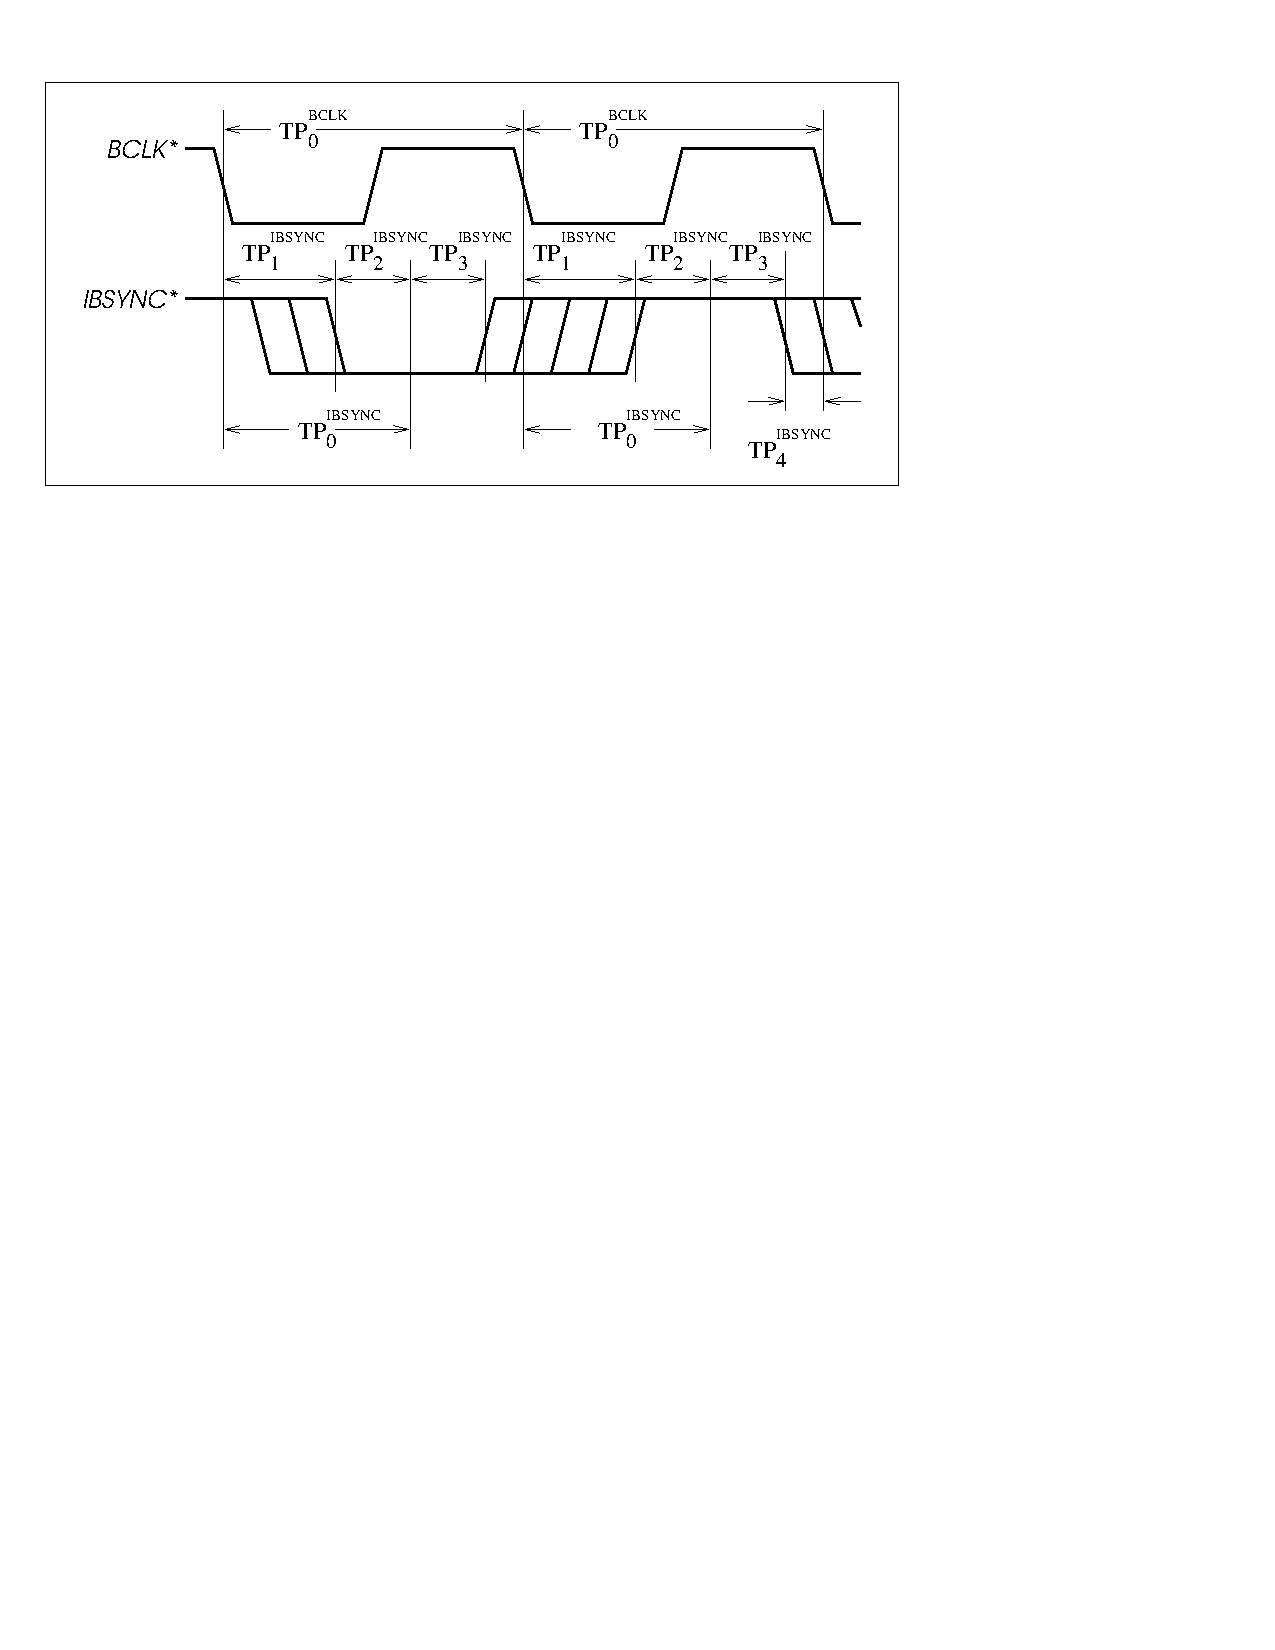
\includegraphics{ch6/FIG/ibsync-time.jpg}}
   \caption{IBSYNC* 신호의 시간규격}\label{figure:ibsync-time}
\end{figure}
%
%
\subsection{인터럽트 버스 중재 동작의 시간 규격}
중재 주기는 버스 클럭 (BCLK*)의 하강점부터 시작되며,
$TP^{IBARB}_0 + TP^{IBARB}_1$동안 신호를 구동해야 한다.
특히 중재결과는 $TP^{IBARB}_0$ 시점에 래치할 수 있도록 안정된 신호를
보장해야 한다.
%\documentstyle[a4]{hbook}
%\begin{document}
%
\begin{table}[htbp]
\caption{인터럽트 중재 버스 신호의 시간규격 요약}\label{table:ibarb-time}
   \begin{center}
   \begin{tabular}{|l|l|r|r|r|} \hline
	timing parameter & name & min & typical & max \\ \hline \hline
	$TP^{BCLK}_0$  & BCLK* cycle time & 59 & 60 & 61 \\ \hline
	$TP^{IBARB}_0$  & arbitration time & 240 & 242 & 244 \\ \hline
	$TP^{IBARB}_1$  & post time & 20 & 30 & 40 \\ \hline
	$TP^{IBARB}_2$  & guard time & 10 & - & - \\ \hline
   \end{tabular}
   \end{center}
\end{table}
%
%\end{document}

\begin{figure}[htb]
    \centerline{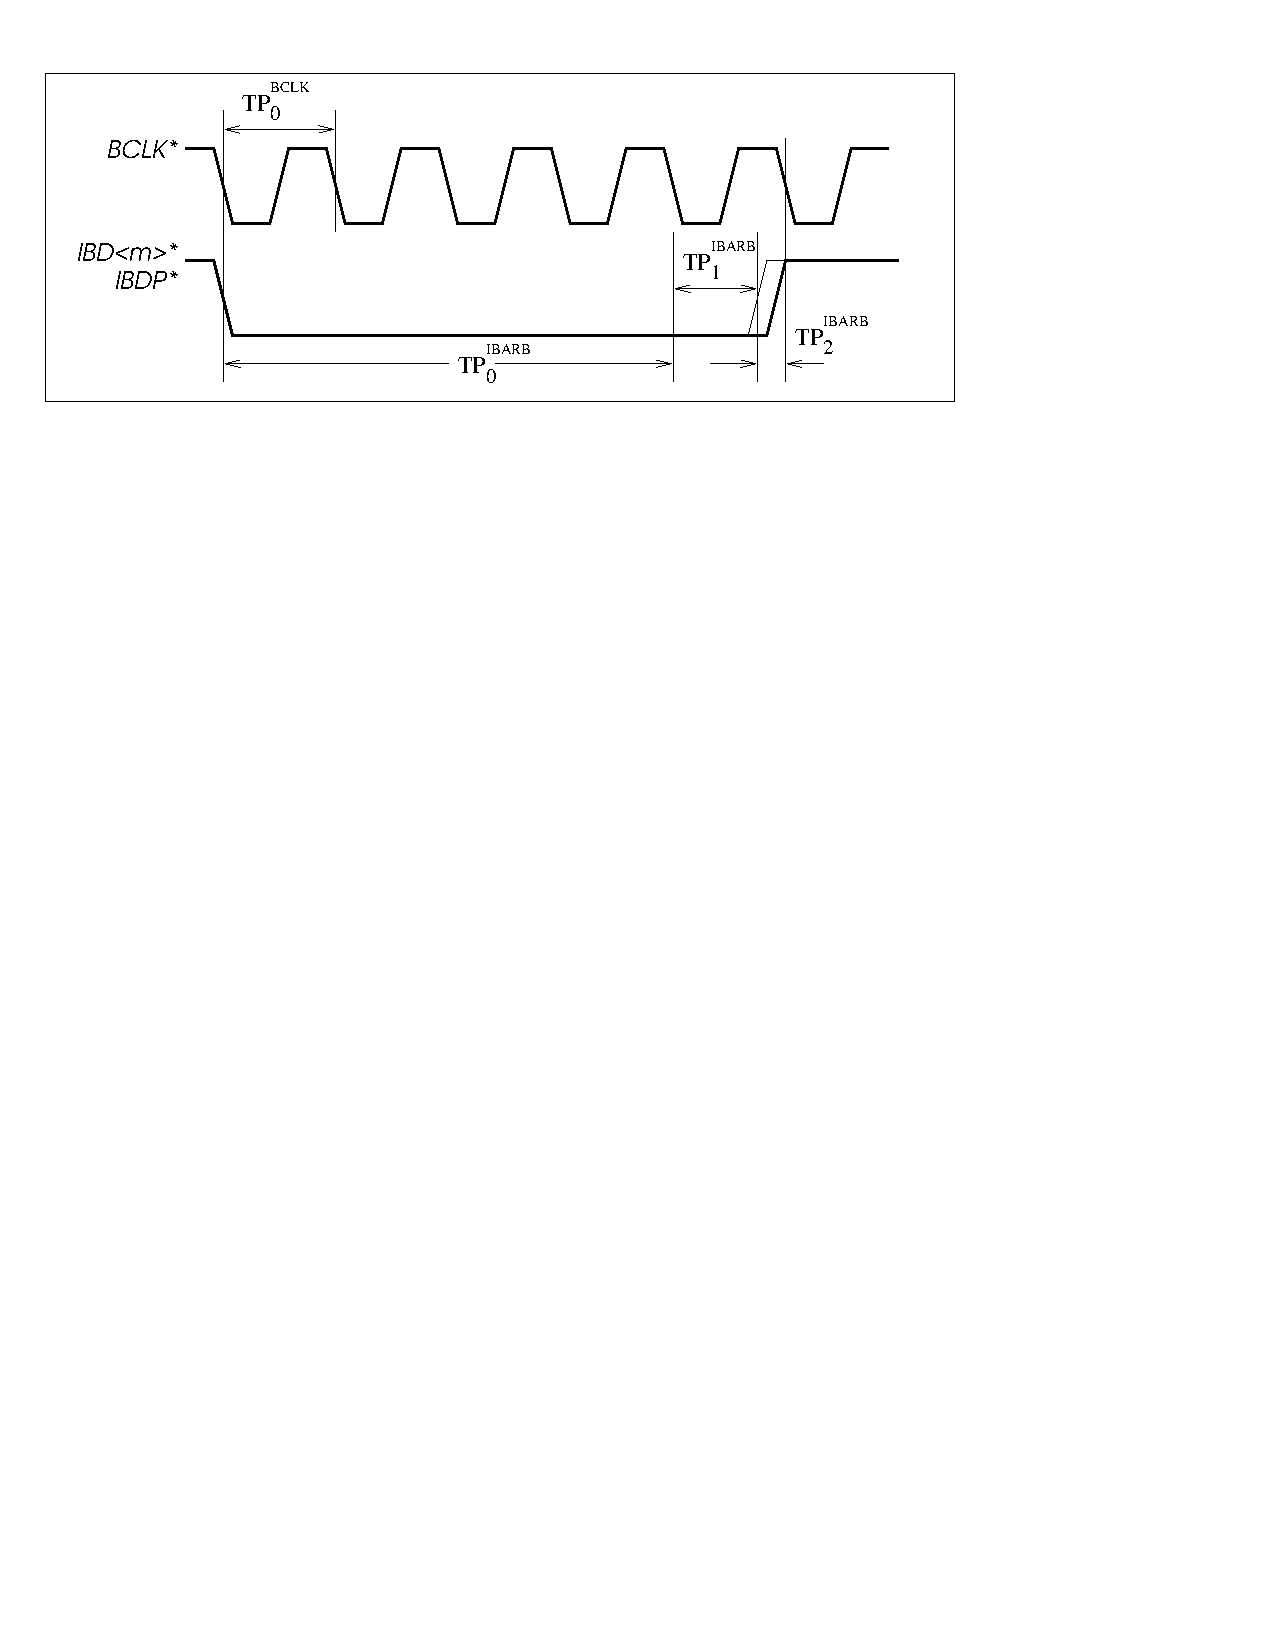
\includegraphics{ch6/FIG/ibarb-time.jpg}}
   \caption{인터럽트 버스 중재 동작의 시간규격}\label{figure:ibarb-time}
\end{figure}
%
\subsection{인터럽트 버스 인터럽트 데이터 전송 주기의 시간 규격}
인터럽트 버스를 통하여 전송하고자 하는 데이터의 신호는
백플레인에 나타나는 버스클럭의 하강점에서 $TP^{IBD}_0$ 후에
안정된 신호를 래치할 수 있도록 셋업시간으로 $TP^{IBD}_2$을
홀드시간으로 $TP^{IBD}_3$를 보장하여야 한다.
그리고 앞과 뒤 신호에 영향을 주지 않도록 $TP^{IBSYNC}_4$을
보장하여야 한다.
%
%\documentstyle[a4]{hbook}
%\begin{document}
%
\begin{table}[htbp]
\caption{인터럽트 버스의 인터럽트 데이터 신호의 시간규격 요약}\label{table:ibd-time}
   \begin{center}
   \begin{tabular}{|l|l|r|r|r|} \hline
	timing parameter & name & min & typical & max \\ \hline \hline
	$TP^{BCLK}_0$ & BCLK* cycle time & 59 & 60 & 61 \\ \hline
	$TP^{IBD}_0$  & IBD{\tt <}n{\tt >}* signal latch point & 38 & 40 & 42 \\ \hline
	$TP^{IBD}_1$  & bus propagation time & - & - & 20 \\ \hline
	$TP^{IBD}_2$  & setup time & 10 & - & - \\ \hline
	$TP^{IBD}_3$  & hold time & 5 & - & - \\ \hline
	$TP^{IBD}_4$  & guard time & 10 & - & - \\ \hline
   \end{tabular}
   \end{center}
\end{table}
%
%\end{document}

\begin{figure}[htb]
    \centerline{\includegraphics{ch6/FIG/ibd-time.jpg}}
   \caption{인터럽트 버스의 데이터 전송의 시간규격}\label{figure:ibd-time}
\end{figure}
%%%

%%%%%

%%%%%
%%Title: HiPi+Bus V0.2 Chapter 7
%%Creator: Ando Ki
%%CreationDate: April 1992
%%FileName: ch7
%%RelatedFile:
%%%%%
\chapter{전기적 규격}
%
%%%%%
%%Title: HiPi+Bus V0.2 Chapter 7
%%Creator: Ando Ki
%%CreationDate: April 1992
%%FileName: sec1
%%RelatedFile: ch7
%%%%%
\section{개요}
전기적 규격에서는 버스에서 공급되는 전원에 대한 전원규격,
전달되는 신호의 전기적 규격을 규정한다.
%\documentstyle[a4]{hbook}
%\begin{document}
%
\begin{table}[htbp]
\caption{전기적 규격 요약}\label{table:elec-spec}
   \begin{center}
   \begin{tabular}{|l l|} \hline
	\multicolumn{2}{|c|}{전원 분배 (Power Distribution)} \\ \hline
	전원의 종류 및 최대 허용 용량 & +5V (30 A/slot), +5V STB (1 A/slot) \\
	콘넥터 핀 당 최대 허용 전류 & 2 A \\ \hline
	\multicolumn{2}{|c|}{BTL 신호의 전기적 특성 (Characteristics of BTL Electrical Signal)} \\ \hline
	최고 전압치 (Steady-state High Level) & 1.9 V 이상  2.1 V 이하 \\
	최저 전압치 (Steady-state Low Level) & 1.1 V 이하 0.0 V 이상 \\ \hline
	\multicolumn{2}{|c|}{BTL 버스 드라이버의 특성 (Characteristics of BTL Bus Driver)} \\ \hline
	기술 (Technology) & BTL (Backplane Transceiver Logic) \\
	전류구동능력 (current driving capability) & 80 $m$A @ $V_{OL}$ \\ \hline
	\multicolumn{2}{|c|}{TTL 신호의 전기적 특성 (Characteristics of TTL Electrical Signal)} \\ \hline
	최고 전압치 (Steady-state High Level) & 2.5 V 이상 \\
	최저 전압치 (Steady-state Low Level) & 0.6 V 이하 \\ \hline
	\multicolumn{2}{|c|}{TTL 버스 드라이버의 특성 (Characteristics of TTL Bus Driver)} \\ \hline
	기술 (Technology) & Advanced Schottky TTL \\
	전류구동능력 (current driving capability) & 64 $m$A @ $V_{OL}$ \\ \hline
	\multicolumn{2}{|c|}{백플레인의 특성 (Characteristics of Backplane)} \\ \hline
	특성 임피던스 (버스클럭/일반신호선) & 50/80 $\Omega$ (홀이 없는 상태) \\
	핀/슬롯 당 최대 허용 용량성 부하 (BTL 신호선)& 15 $p$F \\
	핀/슬롯 당 최대 허용 용량성 부하 (TTL 신호선)& 25 $p$F \\ \hline
	\multicolumn{2}{|c|}{버스 터미네이터의 특성 (Characteristics of Bus Terminator)} \\ \hline
	구성 소자 & Resister, Capacitor \\
	설치 위치 & 백프레인의 양끝 \\ \hline
   \end{tabular}
   \end{center}
\end{table}
%
%\end{document}
%%%%

%
%%%%%

\clearpage
%%%%%
%%Title: HiPi+Bus V0.2 Chapter 7
%%Creator: Ando Ki
%%CreationDate: April 1992
%%FileName: sec2
%%RelatedFile: ch7
%%%%%
\section{전원규격}
백플레인에서 공급해야 되는 주전원으로는 5V TTL 소자를 위한 직류 +5V와
주전원과 무관하게 항상 동작할 필요가 있는 회로를 위해 백플레인에서 공급하는
직류 +5V STB 전원이 있다.

보드 내부 소자의 전원으로 공급되는 PGND와 이것과는 별도로 BTL 버스 구동소자의
기준 전압으로 SGND가 있다.
%\documentstyle[a4]{hbook}
%\begin{document}
%
\begin{table}[htbp]
\caption{전원규격 요약}\label{table:power-spec}
   \begin{center}
   \begin{tabular}{|c|l|c|c|c|} \hline
	mnemonic & description & allowed   & ripple/noise & maximum current \\
	         &             & variation & below 10MHz  & per slot \\ \hline
\hline
	+5V & +5V DC power & +0.25V/-0.125V & 50$m$A & 30A \\ \hline
	+5V STB & +5V DC standby & +0.25V/-0.125V & 50$m$A & 1A \\ \hline
	SGND & signal ground reference & & & \\ \hline
	PGND & power ground reference & & & \\ \hline
   \end{tabular}
   \end{center}
\end{table}
%
%\end{document}
%%%%

%
%%%%%

%%%%%
%%Title: HiPi+Bus V0.2 Chapter 7
%%Creator: Ando Ki
%%CreationDate: April 1992
%%FileName: sec3
%%RelatedFile: ch7
%%%%%
\section{콘넥터의 전기적 규격}
백플레인에 사용하는 콘넥터는 핀과 소켓 형태를 갖는 것을 사용하는데
전원규격에서 정의한 규격을 만족하기 위해서는 {\tt <}표~\ref{table:pin-spec}{\tt >}와
같은 규격을 유지해야된다.
%\documentstyle[a4]{hbook}
%\begin{document}
%
\begin{table}[htbp]
\caption{핀의 전기적 규격}\label{table:pin-spec}
   \begin{center}
   \begin{tabular}{|l|l|} \hline
	핀당 최대 허용 전류 & 2A \\ \hline
	핀당 접촉저항 & 20$m\Omega$ \\ \hline
	최대 허용 전압 & 직류 200V \\ \hline
	절연저항 & 5000 $M\Omega$ \\ \hline
   \end{tabular}
   \end{center}
\end{table}
%
%\end{document}
%%%%

%%%%%
%%%%%

\clearpage
%%%%%
%%Title: HiPi+Bus V0.2 Chapter 7
%%Creator: Ando Ki
%%CreationDate: April 1992
%%FileName: sec4
%%RelatedFile: ch7
%%%%%
\section{BTL 신호의 전기적 규격}
BTL의 정확한 규격은 IEEE Std.1194.1을 따른다. \\
%
BTL 신호의 전기적 규격은 {\tt <}표~\ref{table:btl-spec}{\tt >}와 같다.
%
%
\begin{table}[htbp]
\caption{BTL 신호의 전기적 규격}\label{table:btl-spec}
   \begin{center}
   \begin{tabular}{|l l|l|} \hline
	$V_t$    & typical & 2.0V\\
	$V_{OH}$ & min     & 1.9V\\
	$V_{IH}$ & min     & 1.62V\\
	$V_{IL}$ & max     & 1.47V\\
	$V_{OL}$ & max     & 1.1V\\
	$V_{OL}$ & min     & 0.75V\\
	$GND$    &         & 0.0V\\ \hline
   \end{tabular}
   \end{center}
\end{table}
%

%
신호의 참조전압을 GND 0V라 하고, 터미네이션에 의한 전압이 $V_t$이고,
신호가 구동되지 않은 상태에서의 신호선의 전압은 $V_{OH}^{min}$ 이상이 되어야 하고,
신호선에 신호를 구동할 때 구동소자는 해당 신호선의 전압을 $V_{OL}^{max}$와
$V_{OL}^{min}$ 사이가 되도록 해야 한다.
수신소자의 경우는 $V_{IH}^{min}$ 이상이 되는 전압에 대해서는 높은 전압으로,
$V_{IL}^{max}$ 이하의 전압에 대해서는 낮은 전압으로 받아들여야 한다.
이것을 그림으로 나타내면 {\tt <}그림~\ref{figure:signal-spec-btl}{\tt >}과 같다.
%
\begin{figure}[htb]
    \centerline{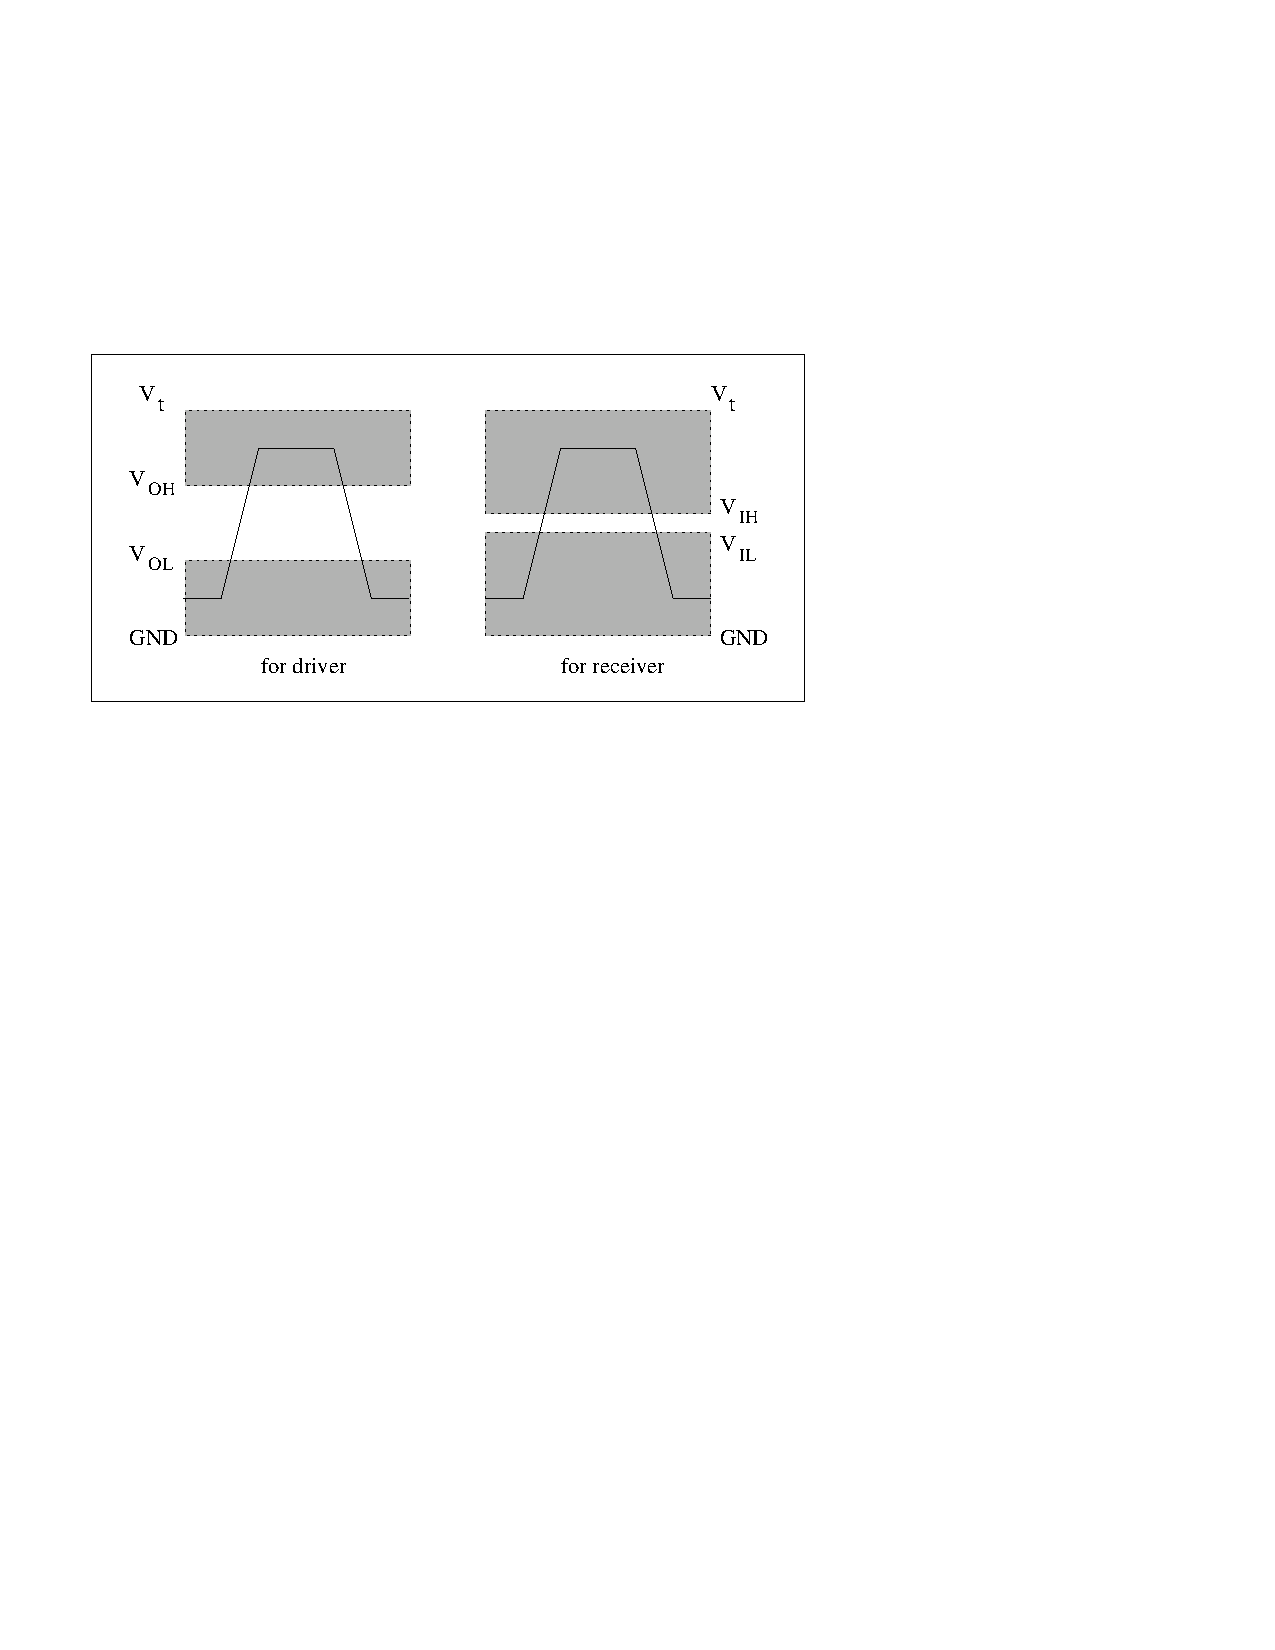
\includegraphics{ch7/FIG/signal-spec.jpg}}
   \caption{BTL 신호선의 전기적 규격}\label{figure:signal-spec-btl}
\end{figure}
%

\subsection{인터페이스 회로의 용량성 부하}
%
BTL 버스에 연결되는 수신소자(receiver), 구동소자(driver), 수신/구동소자(transceiver)의
각 출력단의 용량성 부하는 5$p$F보다 크지 않아야 한다.

\subsection{인터페이스 회로의 누설 전류}
%
백플레인 신호선의 전압이 $V_{OL}$ 영역에 있을때,
해당 신호선에 연결된 인터페이스 소자중 신호를 구동하지 않는 소자의 역방향 누설 전류(negative
leakage current)가 $-250\mu A$보다 작아야 한다.
즉 최대 역방향 누설 전류(maximum negative leakage current)가
$-250\mu A$이다.\\
백플레인 신호선의 전압이 $V_{OH}$ 영역에 있을때,
해당 신호선에 연결된 인터페이스 소자는 제~\ref{sec:voh}장에서 규정하는
최대 순방향 누설 전류(maximum positive leakage current)를 보장해야 한다.

\subsection{구동소자}
%
\subsubsection{구동소자 형태}
%
구동소자는 낮은 전압이 참이어야만 하고, wired-OR 기능이 있어야만 한다.

\subsubsection{정적 부하 전류 (static load current)}
%
백플레인 신호선의 전압이 $V_{OL}$ 일때 구동 소자는 80$m$A의 전류 흡수능력(current
sinking capability)이 있어야 한다.

\subsubsection{구동소자의 $V_{OH}$}\label{sec:voh}
%
$V_{OH}$는 누설 전류, 터미네이션 전압, 부하저항, 그리고 백플레인에 연결된 소자의 수에 의해
결정된다. $V_{OH}^{min}$는 1.9V 이며, 이것은 식 (\ref{eqn:vol})에 의해
정의된다. $V_{OH}^{max}$는 누설 전류가 없는 상황에서 터미네이션 전압 $V_t$가 된다.
%
\begin{table}[htb]
  \begin{eqnarray}
	V_{OH}^{min} & = & V_t - \frac{n \times I_l}{2}
		\times R_t \label{eqn:vol}
  \end{eqnarray}
%
   \begin{center}
   \begin{tabular}{ll}
	$V_t$ & : the termination voltage\\
	$I_l$ & : the maximum positive leakage current\\
	$n$   & : the number of devices on the bus
		(assuming all have the same $I_l$\\
	$R_t$ & : the termination resistor\\
   \end{tabular}
   \end{center}
\end{table}
%

\subsubsection{구동소자의 $V_{OL}$}
%
구동소자의 $V_{OL}$은 전류 흡수가 80$m$A일때 0.75V에서 1.1V사이를
유지해야만 한다.

\subsubsection{천이시간 (transition times)}
%
10\%에서 90\%로의 상승 시간과 90\%에서 10\%로의 하강 시간은 10$n$sec보다
크지 않아야 한다. 그리고 잡음을 최소화하기 위해서는 구동소자가 출력 천이 시간을 3$n$sec보다
작지 않게 해야한다.

\subsection{수신소자}
%
\subsubsection{임계영역 (threshold)}
%
백플레인 신호선에 연결된 모든 수신소자의 수신 임계영역 전압(receiver threshold
voltage)은 엄격히 지켜져야 한다. 1.47V 이하인 경우는 낮은 전압으로,
1.62V이상이면 높은 전압으로 규정한다.
앞에서 규정한 좁은 임계영역전압을 보장함으로써 높은 잡음 허용한계를 얻을 수 있다.

\subsubsection{잡음제거 (noise rejection)}
%
잡음의 영향을 최소화 하기 위해 3$n$sec 미만의 펄스를 제어하는 필터를 수신측에 허용한다.

\subsubsection{입력 클램퍼 (input clamps)}
%
과도한 역저압에 의한 영향을 방지하기 위해 1.5V에 적어도 12$m$A의 클램핑 회로가
수신소자의 입력단에 있어야 한다.
%%%%%
%\end{document}
%%%%%

\clearpage
%%%%%
%%Title: HiPi+Bus V0.2 Chapter 7
%%Creator: Ando Ki
%%CreationDate: April 1992
%%FileName: sec4
%%RelatedFile: ch7
%%%%%
\section{TTL 신호의 전기적 규격}
TTL 신호의 전기적 규격은 {\tt <}표~\ref{table:ttl-spec}{\tt >}와 같다.
%
%
\begin{table}[htbp]
\caption{TTL 신호의 전기적 규격}\label{table:ttl-spec}
   \begin{center}
   \begin{tabular}{|l l|l|} \hline
	$V_t$    & typical & 2.5V\\
	$V_{OH}$ & min     & 2.0V\\
	$V_{IH}$ & max     & 1.8V\\
	$V_{IL}$ & min     & 0.8V\\
	$V_{OL}$ & max     & 0.6V\\
	$GND$    &         & 0.0V\\ \hline
   \end{tabular}
   \end{center}
\end{table}
%

%
신호의 참조전압을 GND 0V라 하고, 터미네이션에 의한 전압이 $V_t$이고,
신호가 구동되지 않은 상태에서의 신호선의 전압은 $V_{OH}^{min}$ 이상이 되어야 하고,
신호선에 신호를 구동할 때 구동소자는 해당 신호선의 전압을 $V_{OL}^{max}$와
$V_{OL}^{min}$ 사이가 되도록 해야 한다.
수신소자의 경우는 $V_{IH}^{min}$ 이상이 되는 전압에 대해서는 높은 전압으로,
$V_{IL}^{max}$ 이하의 전압에 대해서는 낮은 전압으로 받아들여야 한다.
이것을 그림으로 나타내면 {\tt <}그림~\ref{figure:signal-spec-ttl}{\tt >}과 같다.
%
\begin{figure}[htb]
    \centerline{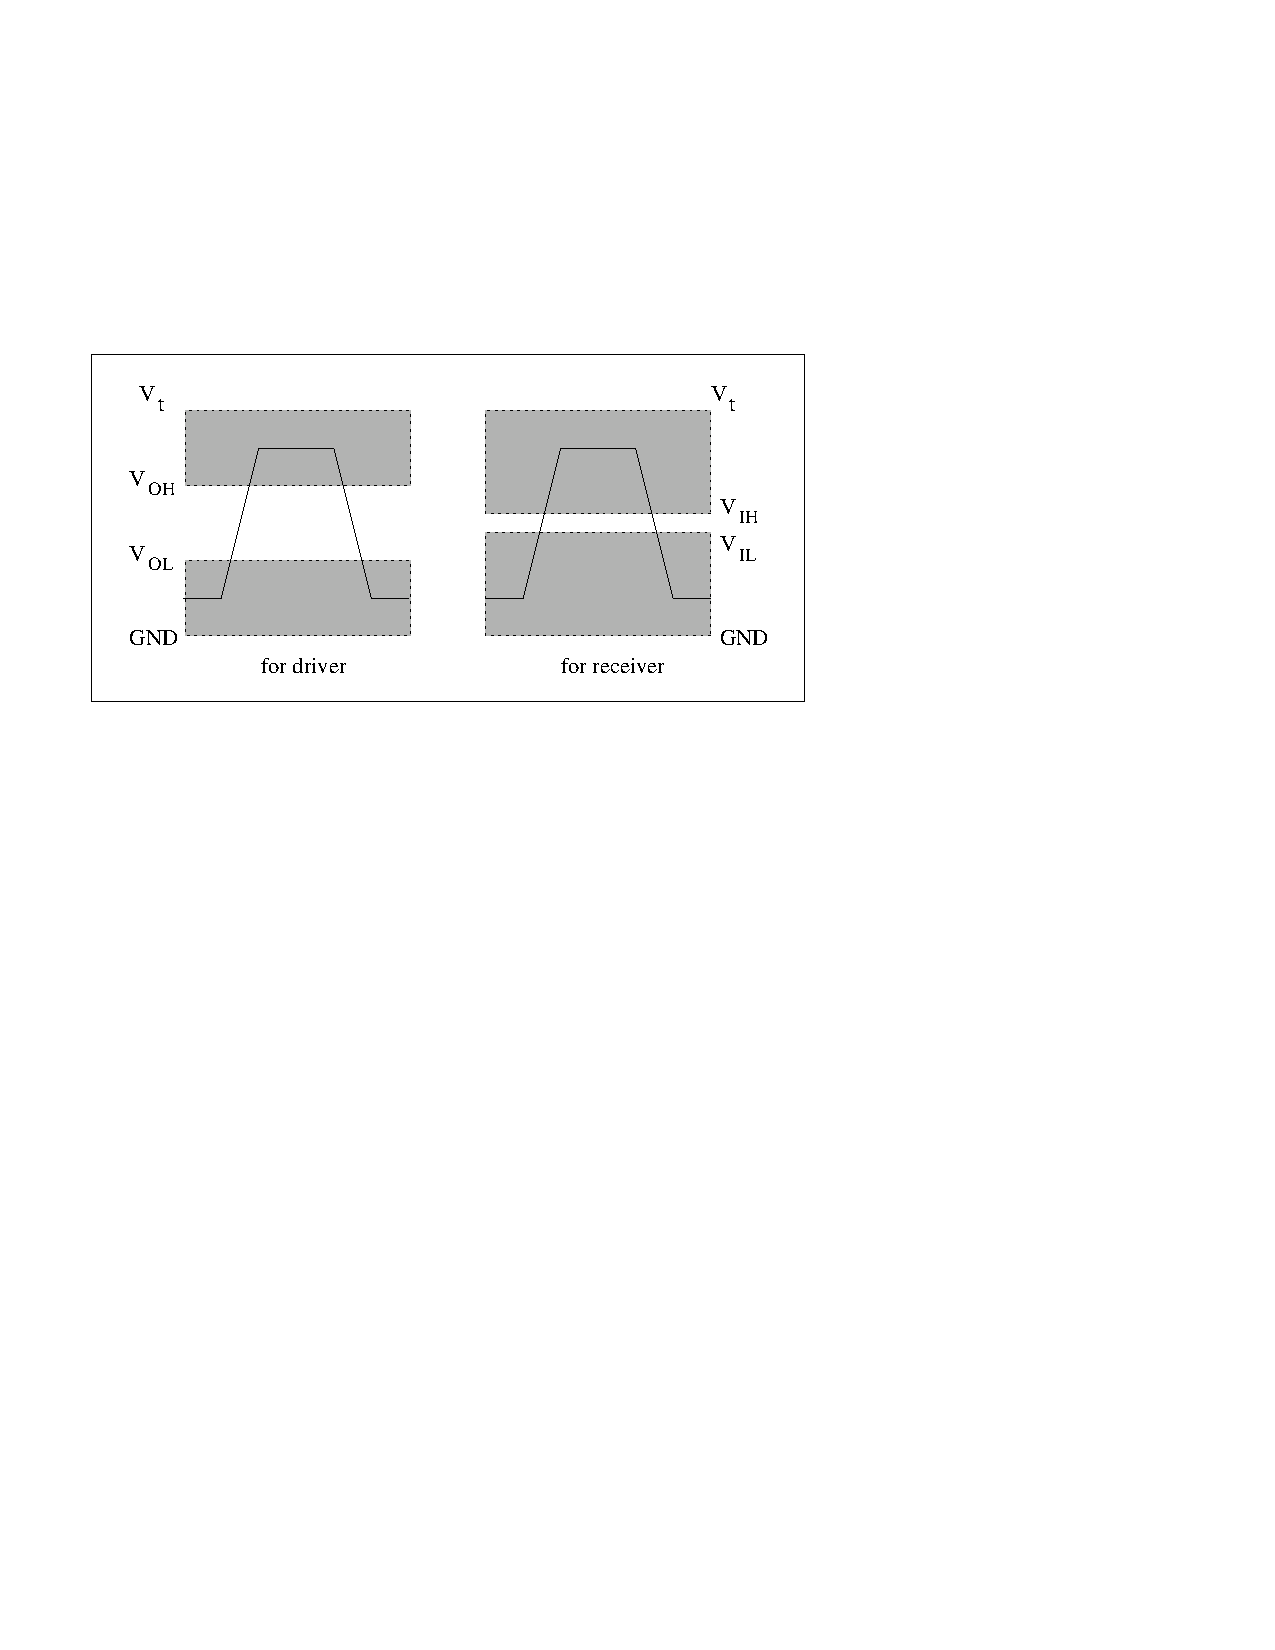
\includegraphics{ch7/FIG/signal-spec.jpg}}
   \caption{TTL 신호선의 전기적 규격}\label{figure:signal-spec-ttl}
\end{figure}
%

\subsection{인터페이스 회로의 용량성 부하}
%
TTL 버스에 연결되는 수신소자(receiver), 구동소자(driver), 수신/구동소자(transceiver)의
각 출력단의 용량성 부하는 15$p$F보다 크지 않아야 한다.

\subsection{구동소자의 종류}
TTL 구동소자의 종류는 totem-pol, three-state, 그리고 open-collector 등
세가지가 있다.
%
%%%%%
%\end{document}
%%%%%

\clearpage
%%%%%
%%Title: HiPi+Bus V0.2 Chapter 7
%%Creator: Ando Ki
%%CreationDate: April 1992
%%FileName: sec5
%%RelatedFile: ch7
%%%%%
\section{백플레인의 특성}
\subsection{백플레인의 특성임피던스}
백플레인의 버스클럭 신호선의 특성임피던스는 50$\Omega$을 유지해야 하고,
나머지 백플레인 신호선의 특성임피던스는 콘넥터를 꽂기 위한 홀이 없는
상태에서 80$\Omega$이어야 하고,
홀과 콘넥터를 연결하였을때 60$\Omega$ 이상이어야 하고,
모든 슬롯에 보드가 꽂힌 상태에서 20$\Omega$이상을 유지해야 한다.
\subsection{터미네이션}
백플레인에는 두가지 터미네이션 방법을 사용한다.
버스클럭의 경우 [그림~\ref{figure:terminator}.a]과 같이 직렬터미네이션 방법을사용하고,
나머지 신호선들은 [그림~\ref{figure:terminator}.b]과 같이 병렬터미네이션 방법을사용한다.
\begin{figure}[htb]
    \centerline{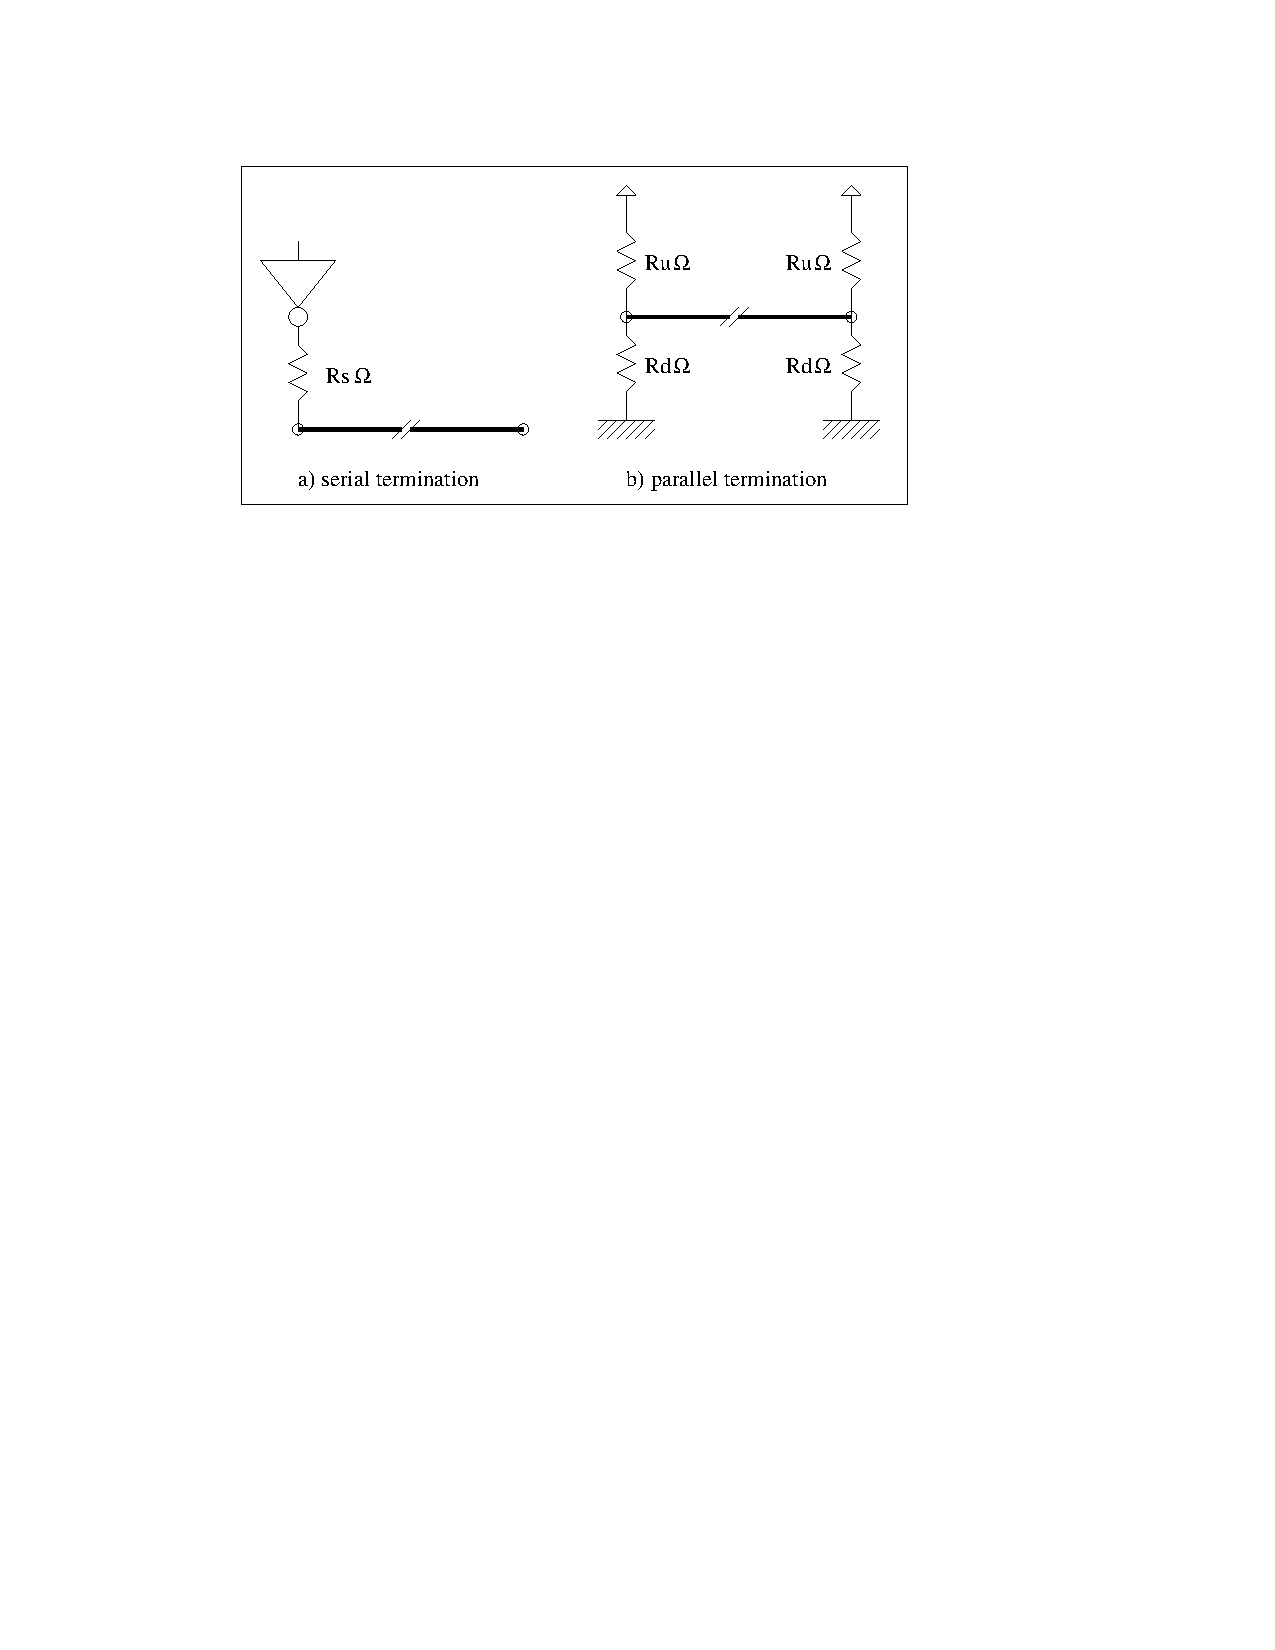
\includegraphics{ch7/FIG/terminator.jpg}}
   \caption{터미네이션 방법}\label{figure:terminator}
\end{figure}
%%%%%
%\end{document}
%%%%%

%%%%%

%%%%%
%%Title: HiPi+Bus V0.2 Chapter 8
%%Creator: Ando Ki
%%CreationDate: September 1992
%%FileName: ch8
%%RelatedFile:
%%%%%
\chapter{기계적 규격}
%
%%%%%
%%Title: HiPi+Bus V0.2 Chapter 8
%%Creator: Ando Ki
%%CreationDate: April 1992
%%FileName: sec1
%%RelatedFile: ch8
%%%%%
\section{개요}
버스의 기계적 규격은 백플레인(backplane), 백플레인에 꽂혀 사용될 보드(board),
백플레인과 보드를 지지하는 서브랙(subrack),
%각 보드간의 전달신호를 안정되게 하는 터미네이터(terminator),
% 보드에 공급될 버스클럭을 공급하는 버스클럭,
각 보드에서 필요로 하는 주전원 전력을 균등하게 공급하도록 하는 파워 바(power bar),
%주전원 이외의 전원 공급을 위한 파워 탭(power tab),
그리고 백플레인과 보드를 연결하는 콘넥터의 규격을 정의한다.
%
\begin{figure}[htb]
    \centerline{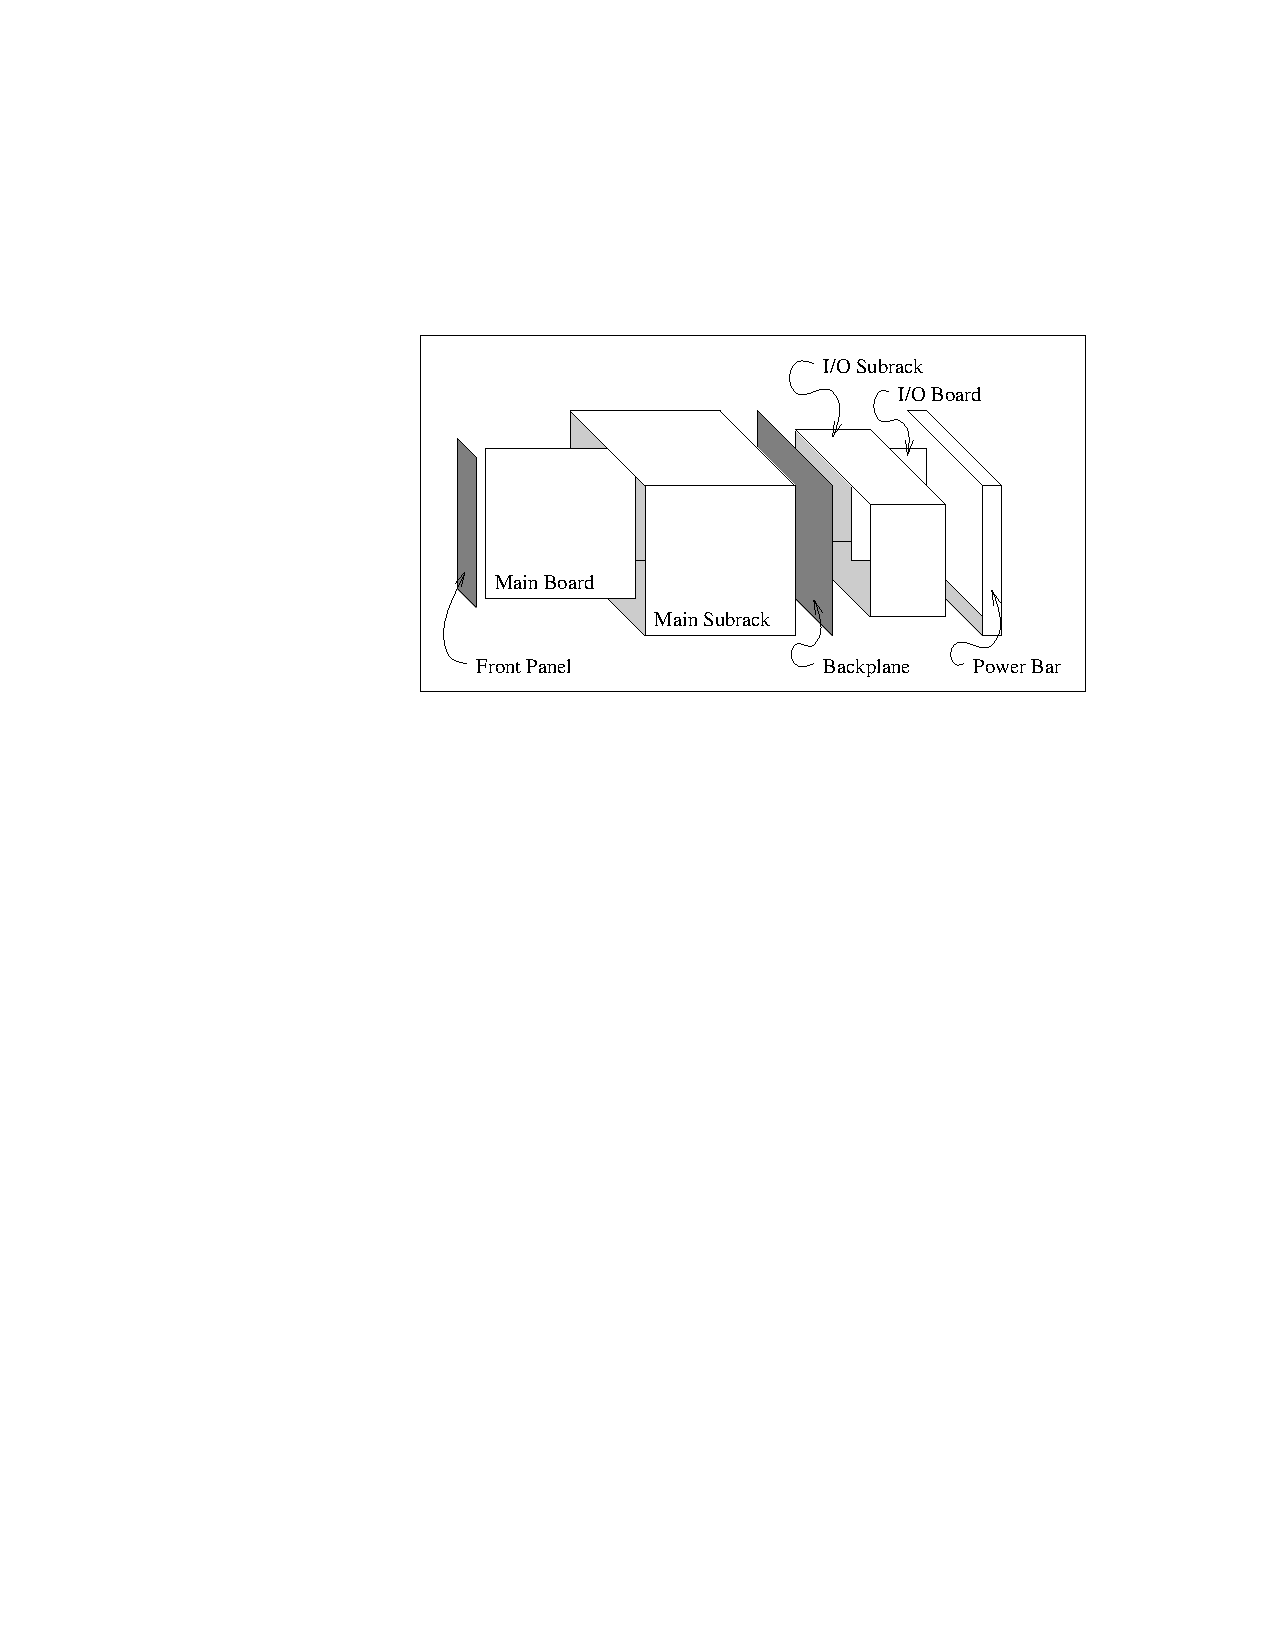
\includegraphics{ch8/FIG/mech-over.jpg}}
   \caption{기계적 장치의 개요}\label{figure:mech-over}
\end{figure}
%
\begin{itemize}
  \item front panel (전면판넬) : HiPi+Bus main board의 전면에 설치되는 전면 판넬이다.
  \item main board (주보드) : HiPi+Bus 백플레인에 꽂히게 될 보드이다.
  \item main subrack (주서브랙) : main board가 백플레인의 슬롯에 꽂힐때 제대로 꽂히도록 지지하는 기구물이다.
  \item backplane (백플레인) : HiPi+Bus 백플레인이다.
  \item I/O subrack (입출력서브랙) : I/O board가 백플레인의 뒷쪽 슬롯에 꽂힐때 제대로 꽂히도록 지지하는 기구물이다.
  \item I/O board (입출력보드) : HiPi+Bus 백플레인 뒷쪽 슬롯에 꽂히게 될 보드로 I/O bus와의 연결을
		용이하게 하기 위한 보드이다.
  \item power bar (파워바) : HiPi+Bus 백플레인의 뒷쪽에 설치되어 백플레인을 통해 백플레인에 꽂히는 모든 보드에
		전원을 공급하고 분배하는 장치이다.
\end{itemize}
%%%%%

%%%%%
%%Title: HiPi+Bus V0.2 Chapter 8
%%Creator: Ando Ki
%%CreationDate: April 1992
%%FileName: sec2
%%RelatedFile: ch8
%%%%%
\section{백플레인}
백플레인의 크기는
%TBD\footnote{추후정의}
525.78$m$m$\times$486.3$m$m$\times$4$m$m
 (width$\times$heigh$\times$thickness)이다.
백플레인에는 보드가 꽂힐 슬롯, 파워바가 연결되어 전원이 공급될 접점,
주서브랙과 입출력서브랙이 고정될 지지영역등이 있다.
그리고 버스클럭 발생회로가 있고, 터미에이션 저항이 설치될 영역이 있다.
백플레인에는 보드가 꽂힐 21개 슬롯(슬롯 0 - 20)이 있고,
각 슬롯에는 보드와의 연결을 위한 백플레인 콘넥터(간접형 숫 콘넥터)가 설치된다.
백플레인을 전면에서 볼 때 가장 왼쪽부터 슬롯 0번(J0), 그 다음이 슬롯 1번(J1)
순이며 가장 오른쪽이 슬롯 20번(J20)이다.
각 슬롯 간의 간격은 0.8 inch 이며, 따라서 슬롯 0번에서 슬롯 20번까지의 거리는
16 inch(406.4 $m$m)이다.
백플레인은 슬롯에 꽂힌 보드들 사이의 신호 전송의 통로를 제공하고
또한 슬롯을 통하여 각 보드에 전원을 공급한다. 각 보드에 공급될 +5V 전원은
파워 바(Power Bar)를 통하여 전원 공급 장치로부터 공급받으며 이 파워 바와의
연결을 위해 백플레인의 위 아래에 각각 20개씩의 접점(+5V용 20개, GND용 20개)이 있다.
또한 +5V STB 전원용 파워 탭(Power Tab) 설치를 위한 접점이 있다.
백플레인은 주서브랙의 뒷면에 설치되며, 그 상세한 규격은 도면으로 첨부한다.
%
%\documentstyle[a4]{hbook}
%\begin{document}
%
\begin{table}[htbp]
\caption{백플레인의 기계적 규격}\label{table:backplane-spec}
   \begin{center}
   \begin{tabular}{|l l|} \hline
	\multicolumn{2}{|c|}{외관상 규격} \\ \hline
	Size & 525.78$m$m$\times$486.3$m$m$\times$4$m$m \\
	Number of Slot & 21 (J0 - J20) \\
	Interval between neighbor slots & 0.8 inch \\
	Interval from J0 to J20 & 16 inch \\ \hline
	\multicolumn{2}{|c|}{Degree of PCB layer} \\ \hline
	Signal & 4 \\
	Clock & 1 \\
	+5 & 2 \\
	SGND & 1 \\
	PGND & 2 \\
	Total & 10 \\ \hline
	\multicolumn{2}{|c|}{전원 공급용 접점수} \\ \hline
	+5V & 20 \\
	GND & 20 \\
	+5V Standby & 1 \\ \hline
   \end{tabular}
   \end{center}
\end{table}
%
%\end{document}
%%%%

%
%%%%%

%%%%%
%%Title: HiPi+Bus V0.2 Chapter 8
%%Creator: Ando Ki
%%CreationDate: April 1992
%%FileName: sec3
%%RelatedFile: ch8
%%%%%
\section{주보드 (Main Board)}
주보드는 백플레인 앞쪽에서 주서브랙안으로 꽂힌다.
주보드의 크기는
400$m$m$\times$455.6$m$m$\times$2$m$m이다.
% (depth$\times$height$\times$thickness)이다.
보드에는 내부 신호선들과 백플레인의 신호선들을 연결하기 위한 보드 콘넥터(board connector, 암 콘넥터)
설치를 위한 영역과, 서브랙에 설치할 때의 가이드 레일(guide rail)을
위한 여유 영역과 전면 판넬(front panel) 설치를 위한 여유 영역이 있고,
이들을 제외한 모든 영역에 부품이 위치할 수 있다. 보드의 상세한 규격은 도면으로 첨부한다.
%
%%%%%

%%%%%
%%Title: HiPi+Bus V0.2 Chapter 8
%%Creator: Ando Ki
%%CreationDate: April 1992
%%FileName: sec4
%%RelatedFile: ch8
%%%%%
\section{입출력보드 (I/O Board)}
입출력보드는 백플레인 뒤쪽에서 입출력서브랙안으로 꽂힌다.
입출력보드의 크기는 127$m$m$\times$362.2$m$m$\times$2$m$m 이다.
% (depth$\times$height$\times$thickness)이다.
보드에는 내부 신호선들과 백플레인의 신호선들을 연결하기 위한 입출력 보드 콘넥터( I/O board connector, 암 콘넥터)
설치를 위한 영역과, 서브랙에 설치할 때의 가이드 레일(guide rail)을
위한 여유 영역이 있고,
이들을 제외한 모든 영역에 부품이 위치할 수 있다. 보드의 상세한 규격은 도면으로 첨부한다.
%
%%%%%

%%%%%
%%Title: HiPi+Bus V0.1 Chapter 8
%%Creator: Ando Ki
%%CreationDate: April 1992
%%FileName: sec5
%%RelatedFile: ch8
%%%%%
\section{파워 바 (Power Bar)와 파워 탭 (Power Tab)}
파워 바(Power Bar)는 백플레인에 꽂히는 21개 보드에 주전원인
+5V, GND 전원을
균등하게 분배되도록 하기 위해 전원 장치로부터 백플레인 사이에 위치하는 
전원 분배용 도체 기구물이며, 그 상세한 규격은 도면으로 첨부한다.

백플레인에는 +5V STB 전원을
연결하기 위한 접점이 있고 이 접점에 설치되는 것이 파워 탭이다.
%파워 탭은 55557-4 또는 55556-4을 사용한다.
%(Part number는 AMP catalog 85-711, Issued 2-86, page 9 참조)
%
%%%%%

%%%%%
%%Title: HiPi+Bus V0.1 Chapter 8
%%Creator: Ando Ki
%%CreationDate: April 1992
%%FileName: sec6
%%RelatedFile: ch8
%%%%%
\section{주서브랙 (Main Subrack)}
백플레인이 고정되고, 백플레인에 꽂힐 주보드들을 지지하기 위한 주서브랙에는
보드가 꽂힐때 용이함을 위해 가이드 레일(guide rail)이 설치된다.
서브랙의 상세한 규격은 도면으로 첨부한다.
%
%%%%%

%%%%%
%%Title: HiPi+Bus V0.1 Chapter 8
%%Creator: Ando Ki
%%CreationDate: April 1992
%%FileName: sec7
%%RelatedFile: ch8
%%%%%
\section{입출력서브랙 (I/O Subrack)}
백플레인이 뒤쪽에 고정되고, 백플레인에 꽂힐 입출력보드들을 지지하기 위한 입출력서브랙에는
보드가 꽂힐때 용이함을 위해 가이드 레일(guide rail)이 설치된다.
서브랙의 상세한 규격은 도면으로 첨부한다.
%
%%%%%

%%%%%
%%Title: HiPi+Bus V0.1 Chapter 8
%%Creator: Ando Ki
%%CreationDate: April 1992
%%FileName: sec8
%%RelatedFile: ch8
%%%%%
\section{콘넥터}
시스템 버스 백플레인과 보드를 연결하기 위해 간접형 콘넥터(Indirect Connector)를 사용한다.
콘넥터는 340핀(85핀 $\times$ 4줄)(전원 핀을 따로) 주콘넥터와
160핀(40핀 $\times$ 4줄)(전원 핀 포함) 입출력 콘넥터로 백플레인 쪽에는 
숫콘넥터(버스 콘넥터), 보드 쪽에는 암콘넥터(보드 콘넥터)를 사용한다.
특히, 버스 콘넥터는 press-fit 형태의 콘넥터를 사용하며,
각슬롯의 아래쪽 160핀용 콘넥터는 백플에인 뒤쪽에서 보드가 설치
될 수 있도록 다리가 긴 콘넥터를 사용한다.
%
%%%%%

%%%%%

\appendix
%%%%%
%%Title: HiPi+Bus V0.2 Chapter 1
%%Creator: Ando Ki
%%CreationDate: September 1992
%%FileName: ap
%%RelatedFile:
%%%%%
%\documentstyle[11pt,doublespace,a4wide,psfig]{hbook}
%\setstretch{1.2}
%\pagestyle{headings}
%\begin{document}
%\def\HB{HiPi+Bus}	% define system bus name
%\def\HC{HICOM}		% define system name
%
%\pagenumbering{roman}
%\tableofcontents
%\listoffigures
%\listoftables
%
%\newpage
%\pagenumbering{arabic}
%\setcounter{chapter}{7}
%\setcounter{page}{94}
%
%\appendix
\chapter{HiPi+Bus 신호선과 핀할당}
%
%\clearpage
%\section{HiPi+Bus 신호선들}\label{apsec:signals}
%\documentstyle[11pt,a4]{hbook}
%\begin{document}
%
\begin{table}[htbp]
\section{HiPi+Bus 신호선들}
%\caption{신호선들}\label{table:signals}
   \begin{center}
\begingroup
\setlength{\tabcolsep}{6pt} % Default value: 6pt
\renewcommand{\arraystretch}{0.9} % Default value: 1
   \begin{tabular}{|l|l|r|l|} \hline
Bus&Mnemonic & Size & Name \\ \hline \hline
     & {\bf ABREQ{\tt <}12..0{\tt >}*} & 13 & Address Bus Request \\
     & {\bf ABINH*}                    & 1 & Address Bus Arbitration Inhibition \\
중재버스 & {\bf WRINH*}                    & 1 & Write Cycle Inhibition \\
     & {\bf DBREQ{\tt <}8..0{\tt >}*}  & 9 & Data Bus Request \\
     & {\bf DBINH*}                    & 1 & Data Bus Arbitration Inhibition \\
     & {\bf PCW*}                      & 1 & Priority Change Window \\ \hline
         & {\bf A{\tt <}31..4{\tt >}*}     & 28 & Address \\
         & {\bf AP{\tt <}3..0{\tt >}*}     & 4 & Address Parity \\
         & {\bf SI{\tt <}7..0{\tt >}*}     & 8 & Source Identification \\
         & {\bf SIP*}                      & 1 & Source Identification Parity \\
데이터전송버스  & {\bf AS{\tt <}2..0{\tt >}*}     & 3 & Address Space \\
(어드레스버스) & {\bf TT{\tt <}4..0{\tt >}*}     & 5 & Transfer Types \\
         & {\bf STP*}                      & 1 & Space + Types Parity \\
         & {\bf BE{\tt <}15..0{\tt >}*}    & 16 & Byte Enable \\
         & {\bf BEP{\tt <}1..0{\tt >}*}    & 2 & Byte Enable Parity \\
         & {\bf AE*}                       & 1 & Address Cycle Enable \\ \hline
         & {\bf D{\tt <}127..0{\tt >}*}    & 128 & Data \\
데이터전송버스  & {\bf DP{\tt <}15..0{\tt >}*}    & 16 & Data Parity \\
(데이터버스)  & {\bf DI{\tt <}7..0{\tt >}*}     & 8 & Destination Identification \\
         & {\bf DIP*}                      & 1 & Destination Identification Parity \\
         & {\bf DE*}                       & 1 & Data Cycle Enable \\ \hline
        & {\bf AACK{\tt <}1..0{\tt >}*}   & 2 & Address Acknowledge \\
        & {\bf SHD*}                      & 1 & Hit on Shared Line \\
        & {\bf DTY*}                      & 1 & Hit on Dirty Line \\
데이터전송버스 & {\bf SNK*}                      & 1 & Snoop No Acknowledge \\
(상태버스)  & {\bf ITV*}                      & 1 & Intervention \\
        & {\bf LCR*}                      & 1 & Hit on Interlocked Region \\
        & {\bf DACK*}                     & 1 & Data Acknowledge \\
        & {\bf CDK*}                      & 1 & Cache Data Acknowledge \\
        & {\bf SPIN{\tt <}3..0{\tt >}*}   & 4 & Spin lock list number \\
        & {\bf BSY{\tt <}7..0{\tt >}*}    & 8 & Busy Status Line \\ \hline    
인터럽트 & {\bf IBSYNC*}                   & 1 & Interrupt Bus Sync. \\
전송버스 & {\bf IBD{\tt <}7..0{\tt >}*}    & 8 & Interrupt Bus Data \\
     & {\bf IBDP*}                     & 1 & Interrupt Bus Data Parity \\ \hline
       & {\bf BCLK*}   & 1 & Bus Clock \\
유틸리티버스 & {\bf RST*}                      & 1 & System Reset \\
       & {\bf SFAIL*}                    & 1 & System Fail \\
       & {\bf GA{\tt <}4..0{\tt >}*}     & 5 & Geographical Slot Address \\
       & {\bf Tx{\tt <}4..0{\tt >}}     & 5 & Boundary Scan Option \\ \hline
       & {\it total\/} & 293 & \\
\hline
   \end{tabular}
\endgroup
   \end{center}
\end{table}
%
%\end{document}
%%%%

%
\clearpage
\section{HiPi+Bus 핀할당}\label{apsec:pin-assign}
\input{appendix/TBL/pin-assign}
%
%\end{document}
%%%%%

\clearpage
\input{appendix/TEXT/apB}
%%%%%
\end{document}
%%%%%
